\documentclass[12pt]{book}

% This first part of the file is called the PREAMBLE. It includes
% customizations and command definitions. The preamble is everything
% between \documentclass and \begin{document}.

\usepackage[margin=1in]{geometry}  % set the margins to 1in on all sides
\usepackage{graphicx}              % to include figures
\usepackage{amsmath}               % great math stuff
\usepackage{amsfonts}              % for blackboard bold, etc
\usepackage{amsthm}                % better theorem environments
\usepackage{amssymb}
\usepackage[activeacute, spanish]{babel}
\usepackage[utf8]{inputenc}
\usepackage{hyperref}
\usepackage{multicol}
\usepackage{mathrsfs}
\usepackage{tikz-cd}
\usetikzlibrary{calc}
\usetikzlibrary{matrix}

\setcounter{tocdepth}{3}% to get subsubsections in toc

\let\oldtocsection=\tocsection

\let\oldtocsubsection=\tocsubsection

\let\oldtocsubsubsection=\tocsubsubsection

% various theorems, numbered by section

\newtheorem{teo}{Teorema}[section]
\newtheorem{lem}[teo]{Lema}
\newtheorem{prop}[teo]{Proposición}
\newtheorem{cor}[teo]{Corolario}

\theoremstyle{definition}
\newtheorem{conj}[teo]{Conjetura}
\newtheorem{obs}[teo]{Observación}
\newtheorem{defn}[teo]{Definición}
\newtheorem{ax}[teo]{Axioma}
\newtheorem{ex}[teo]{Ejemplo}

\newcommand{\bd}[1]{\mathbf{#1}}  % for bolding symbols
\newcommand{\CC}{\mathbb{C}}
\newcommand{\RR}{\mathbb{R}}      % for Real numbers
\newcommand{\ZZ}{\mathbb{Z}}      % for Integers
\newcommand{\NN}{\mathbb{N}}
\newcommand{\QQ}{\mathbb{Q}}
\newcommand{\FF}{\mathbb{F}}
\newcommand{\PP}{\mathscr{P}}
\newcommand{\Rel}{\mathscr{R}}
\newcommand{\col}[1]{\left[\begin{matrix} #1 \end{matrix} \right]}
\newcommand{\comb}[2]{\binom{#1^2 + #2^2}{#1+#2}}
\newcommand{\eps}{\varepsilon}
\renewcommand{\hom}{\mathrm{Hom}}
\let\oldemptyset\emptyset
\let\emptyset\varnothing
\DeclareMathOperator{\id}{id}
\DeclareMathOperator{\mcm}{mcm}
\DeclareMathOperator{\mcd}{mcd}
\DeclareMathOperator{\ord}{ord}
\DeclareMathOperator{\im}{im}
\DeclareMathOperator{\End}{End}
\DeclareMathOperator{\Aut}{Aut}
\DeclareMathOperator{\sg}{sg}
\DeclareMathOperator{\coker}{coker}
\DeclareMathOperator{\Obj}{Obj}
\DeclareMathOperator{\rank}{rk}
\DeclareMathOperator{\gr}{gr}
\DeclareMathOperator{\car}{car}
\DeclareMathOperator{\Nil}{Nil}
\DeclareMathOperator{\spec}{Spec}
\DeclareMathOperator{\ev}{ev}
\DeclareMathOperator{\ann}{Ann}
\def\acts{\curvearrowright}
\def\stca{\curvearrowleft}



\begin{document}
\pagenumbering{roman}\clearpage\tableofcontents\newpage\pagenumbering{arabic}

\chapter{Topología General}

\section{Definiciones Básicas:}

\begin{defn}
Sea $X$ un conjunto. Una \textbf{topología} $\tau$ sobre $X$ es un subconjunto de $\PP(X)$ tal que:
\begin{itemize}
\item Si $U_i\in \tau$ para todo $i\in I$, entonces $\displaystyle\bigcup_{i\in I} U_i \in \tau$.
\item Si $U_i\in \tau$ para todo $i\in I$ con $I$ finito, entonces $\displaystyle\bigcap_{i\in I} U_i \in \tau$.
\item $\emptyset\in\tau$ y $X\in\tau$.
\end{itemize}
\end{defn}

\begin{obs}
Si tomo $I=\emptyset$ en el primer ítem, se deduce que $\emptyset\in\tau$ y si tomo $I=\emptyset$ en el segundo ítem, se deduce que $X\in \tau$. Por lo tanto, si podemos pensar en intersecciones/uniones vacías la tercera condición es redundante.
\end{obs}

\begin{defn}
Un \textbf{espacio topológico} es un par $(X,\tau)$ donde $\tau$ es una topología sobre $X$. Los elementos de $X$ se llaman \textbf{puntos} y los elementos de $\tau$ se llaman \textbf{abiertos}.
\end{defn}

\begin{ex}
Sea $X$ un conjunto y $\tau = \{\emptyset, X\}$. Esta topología es la más chica que se puede definir sobre $X$ y se llama la \textbf{topología indiscreta}. Por otra parte, si tomamos $\tau = \PP(X)$ entonces esta es la topología más grande que se puede definir sobre $X$ y se llama la \textbf{topología discreta}.

Sea $X$ un conjunto y $d$ una métrica (Es decir, una función $d:X\times X\to \RR$ tal que $d(x,y)\geq 0$, $d(x,y)=0$ si y sólo si $x=y$, $d(x,y)=d(y,x)$ y $d(x,y)+d(y,z) \geq d(x,z)$). Esta métrica $d$ nos define una topología $\tau = \{U\in\PP(X) : \forall x\in U \; \exists \varepsilon >0 \text{ tal que } B(x,\varepsilon) \subseteq U\}$ donde $B(x,r)= \{y\in X : d(x,y) < r\}$ es la bola de centro $x$ y radio $r$. Notemos que en esta topología, para todo $x\in X$ y $\varepsilon > 0$, las bolas abiertas $B(x,\varepsilon)$ son abiertas (En efecto, si tomamos $y\in B(x,\varepsilon)$, debemos tomar $B(y,r)$ con $r< \varepsilon - d(x,y)$ y ver, usando la desigualdad triangular, que en efecto queda contenida en $B(x,\varepsilon)$).

Si $(X,\tau)$ es un espacio topológico y $X'\subseteq X$ es un subconjunto, entonces podemos definir $\tau' = \{U\cap X' : U\in \tau\}$. Esta topología sobre $X'$ es la denominada la \textbf{topología subespacio}.

Si $X$ es un conjunto, definimos $\tau = \{U\in \PP(X) : U^c \text{ es finito}\}\cup \{\emptyset\}$. Esta topología se denomina la \textbf{topología cofinita}.

Si $X=\{a,b\}$ podemos considerar la topología de Sierpinski $\tau = \{\emptyset, \{a\},X\}$. Notemos que no existe ninguna métrica $d$ sobre $X$ que defina estos abiertos, pues $\{b\} = B(b, d(a,b)/2)$ que es abierto.
\end{ex}

\begin{defn}
Un espacio topológico $(X,\tau)$ se dice \textbf{metrizable} si la topología $\tau$ coincide con la topología inducida por una métrica $d$ sobre $X$.
\end{defn}

\begin{ex}
Si $(X,\PP(X))$ es un espacio topológico provisto de la topología discreta, entonces es metrizable con la distacia discreta $d(x,y)=\delta_{x,y}$. Por otra parte, como vimos en el ejemplo anterior, $X=\{a,b\}$ con la topología de Sierpinski no es un espacio topológico metrizable.
\end{ex}

\begin{defn}
Si $(X,\tau)$ es un espacio topológico, un conjunto $F\subseteq X$ es \textbf{cerrado} si su complemento $F^c\in \tau$ es abierto.
\end{defn}
\begin{obs}
Notemos que podemos definir a una topología tanto por sus abiertos como por sus cerrados. En efecto:
\begin{itemize}
\item Si $F_i$ es cerrado para todo $i\in I$, entonces $\displaystyle\bigcap_{i\in I} F_i$ es cerrado.
\item Si $F_i$ es cerrado para todo $i\in I$, $I$ finito, entonces $\displaystyle\bigcup_{i\in I}F_i$ es cerrado.
\item $\emptyset$ y $X$ son cerrados.
\end{itemize}
Si $\{F_i\}_{i\in I}\subseteq\PP(X)$ es una familia que verifica esas tres condiciones entonces $\tau = \{F_i^c\}_{i\in I}$ es una topología sobre $X$ y recíprocamente si $\tau$ es una topología $\{U^c : U\in \tau\}$ es una familia que cumple esas tres condiciones.
\end{obs}

\begin{ex}
A veces es más conveniente definir a una topología por sus cerrados. Por ejemplo, si $k$ es un cuerpo y $A=k[x_1,\ldots , x_n]$, para cada $S\subseteq A$ definimos $F_S = \{x\in k^n : p(x)=0\;\forall p\in S\}$. Vamos a definir a los $F_S$ como los cerrados de una topología. Para eso, debemos corroborar que se cumplen las tres condiciones:

Sea $\{S_i\}_{i\in I}\subseteq k[x_1,\ldots , x_n]$. Entonces $\displaystyle\bigcap_{i\in I}F_{S_i} = \{x\in k^n : p(x) = 0 \; \forall p\in S_i \;\forall i\in I\}$. Por lo tanto, la intersección de elementos de $\{F_S\}_{S\subseteq A}$ está en el conjunto.

Ahora, si $I$ es un conjunto finito, para ver que la unión finita de elementos del conjunto está, bastará ver que la unión de dos elementos está (pues después sólo habría que hacer una sencilla inducción). Sean $S_1,S_2\subseteq A$. Entonces, es fácil ver que $F_{S_1}\cup F_{S_2} = F_S$ donde $S=\{pq : p\in S_1, q\in S_2\}$. En efecto, veamos la doble inclusión: Sea $x\in F_{S_1}$. Para cualesquiera $p\in S_1, q\in S_2$ tenemos que $p(x)q(x) = (pq)(x) = 0$, y así $x\in F_S$. Si $x\in F_{S_2}$ el resultado es análogo, y así $F_{S_1}\cup F_{S_2}\subseteq F_S$. Ahora, sea $x\in F_S$ tal que $x\notin F_{S_1}\cup F_{S_2}$. Entonces, existen $p\in S_1, q\in S_2$ tales que $p(x)\neq 0$ y $q(x)\neq 0$. Pero como $pq\in S$ y $x\in F_S$ debemos tener que $(pq)(x) = p(x)q(x) = 0$ y así $p(x)=0$ o $q(x)=0$. Absurdo.

Finalmente, $\emptyset = F_{\{1\}}$ y $k^n = F_{\{0\}}$.

Esta topología se denomina la \textbf{topología de Zariski}.

\end{ex}

\begin{defn}
Sea $(X,\tau)$ un espacio topológico y $A\subseteq X$. Se define el \textbf{interior} de $A$ como $A^\circ = \displaystyle\bigcup_{U\in \tau, U\subseteq A} U$. Es decir, es el abierto más grande que está contenido en $A$. Se define la \textbf{clausura} de $A$ como $\overline{A}=\displaystyle\bigcap_{F^c\in \tau, F\supseteq A} F$. Es decir, es el cerrado más chico que contiene a $A$. Si $x\in A^\circ$ entonces se dice que es un \textbf{punto interior} y si $x\in \overline{A}$ se dice que es un \textbf{punto de adherencia}.
\end{defn}

\begin{prop}
Valen las siguientes propiedades:
\begin{enumerate}
\item $A^\circ \subseteq A$.
\item Si $B$ es abierto y $B\subseteq A$ entonces $B\subseteq A^\circ$.
\item Si $A_1\subseteq A_2$ entonces $A_1^\circ \subseteq A_2^\circ$.
\item $A\subseteq \overline{A}$.
\item Si $C$ es cerrado y $A\subseteq C$ entonces $\overline{A}\subseteq C$.
\item Si $A_1\subseteq A_2$ entonces $\overline{A_1}\subseteq \overline{A_2}$.
\item $(\overline{A})^c = (A^c)^\circ$.
\item $\overline{A^c} = (A^\circ)^c$.
\item $(A\cap B)^\circ = A^\circ \cap B^\circ$.
\item $A^\circ \cup B^\circ \subseteq (A\cup B)^\circ$. (La igualdad no necesariamente vale, por ejemplo $X=\RR$ con la topología usual, $A=\RR-\{0\}$ y $B=\{0\}$.
\item $\overline{A\cup B} = \overline{A}\cup \overline{B}$.
\item $\overline{A\cap B}\subseteq \overline{A}\cap\overline{B}$. (La igualdad no necesariamente vale, por ejemplo $X=\RR$ con la topología usual, $A=\RR-\{0\}$ y $B=\{0\}$.
\item Si $A\subseteq X$, entonces $x\in \overline{A}$ si y sólo si para todo $U$ abierto con $x\in U$ tenemos $A\cap U\neq \emptyset$.
\end{enumerate}
\begin{proof}

Las demostraciones de 1),2) y 3) son obvias, y las de 4),5),6) son similares a las primeras tres. Para probar 7) veamos que vale la doble inclusión. En efecto, sea $x\in \overline{A}^c$. Esto quiere decir que $x\notin \overline{A}$, y así existe $F$ cerrado con $A\subseteq F$ tal que $x\notin F$. Sea $U\in F^c$. Entonces $x\in U$ y $U\subseteq A^c$. Por lo tanto, $x\in (A^c)^\circ$. Para ver la otra inclusión, sea $x\in (A^c)^\circ$. Entonces, existe $U$ abierto con $x\in U\subseteq A^c$. Sea $F=U^c$. Por lo tanto, $x\notin F$, $F\supseteq A$ y así $x\notin \overline{A}$, lo que implica $x\in (\overline{A})^c$ como queríamos.

La 8) sigue de 7) aplicada a $A^c$: Es decir, $\overline{A^c}^c = A^\circ$ y tomando complemento $\overline{A^c} = (A^\circ)^c$.

Para la 9) también probamos la doble inclusión: Es trivial que $(A\cap B)^\circ \subseteq A^\circ \cap B^\circ$, pues $A\cap B \subseteq A,B$ y usamos 3). Para la otra inclusión, notemos que $A^\circ\cap B^\circ$ es abierto y $A^\circ \cap B^\circ \subseteq A\cap B$ y por 2) sigue lo deseado.

La 10) es evidente y la 11) es similar a la 9). La 12) también es evidente.

Finalmente, para probar la 13) veamos la doble implicación: $(\Longrightarrow)$ Sea $U$ abierto con $x\in U$. Si tuviéramos $A\cap U=\emptyset$ entonces $U\subseteq A^c$. Sea $F=U^c$. Entonces, $A\subseteq F$. Pero $x\notin F$. Absurdo pues $x\in \overline{F}$.
$(\Longleftarrow)$ Sea $F$ cerrado con $F\supseteq A$ tal que $x\notin F$. Sea $U=F^c$ abierto y así $x\in U$. Por lo tanto, $A\cap U\neq \emptyset$ y así $A\not\subseteq F$. Absurdo.

\end{proof}
\end{prop}

\begin{defn}
Un conjunto $A\subseteq X$ se dice \textbf{denso} si $\overline{A}=X$.
\end{defn}

\begin{defn}
Si $A\subseteq X$ se define la frontera $\mathrm{Fr}(A) = \overline{A}\cap \overline{A^c}$.
\end{defn}

\begin{obs}
Notemos que $A^\circ \cap \mathrm{Fr}(A)=\emptyset$ pues $\mathrm{Fr}(A)\subseteq \overline{A^c} = (A^\circ)^c$.

Además, $A^\circ \sqcup \mathrm{Fr}(A) = \overline{A}$ pues $\overline{A} = \overline{A}\cap (A^\circ \sqcup (A^\circ)^c) = A^\circ \sqcup (\overline{A}\cap \overline{A^c})$.

Finalmente, $X=A^\circ \sqcup \mathrm{Fr}(A) \sqcup (A^c)^\circ$ usando las dos afirmaciones anteriores.
\end{obs}

\begin{defn}
Sea $(X,\tau)$ un espacio topológico. Una \textbf{base} $\mathscr{B}$ de la topología $\tau$ es un conjunto $\mathscr{B}\subseteq \tau$ tal que para todo $U\in\tau$ existen $(U_i)_{i\in I}\subseteq \mathscr{B}$ de modo que $U = \displaystyle\bigcup_{i\in I}U_i$.
\end{defn}

\begin{ex}
En $\RR$ con la topología usual, $\mathscr{B}=\{(a,b) : a<b\}$ es una base. En $\RR^n$ con la topología usual, $\mathscr{B}=\{B(x,\varepsilon) : x\in\RR^n, \varepsilon > 0\}$ es una base. También, $\mathscr{B}' = \{B(q,\frac{1}{n}) : q\in\QQ^n , n\in\NN\}$ es una base de $\RR^n$. En efecto, si $U$ es un abierto $x\in U$ existe un $\varepsilon >0$ tal que $B(x,\varepsilon)\subseteq U$. Existe $k_x\in\NN$ tal que $\dfrac{1}{k_x}<\dfrac{\varepsilon}{2}$ y $q_x\in\QQ^n$ de modo que $d(x,q_x)<\dfrac{1}{k_x}$. Entonces por desigualdad triangular $B(q_x,\frac{1}{k_x})\subseteq U$ y así $U=\displaystyle\bigcup_{x\in U} B\left(q_x,\frac{1}{k_x}\right)$.
\end{ex}

\begin{prop}
Si $\mathscr{B}$ es una base de $\tau$ entonces: \begin{itemize} \item Para todos $U_1,U_2\in\mathscr{B}$, $x\in U_1\cap U_2$ existe $U_3\in\mathscr{B}$ tal que $x\in U_3\subseteq U_1\cap U_2$. \item $\forall x\in X$ existe $U\in \mathscr{B}$ tal que $x\in U$.\end{itemize}

Recíprocamente, si $X$ es un conjunto $\mathscr{B}\subseteq \PP(X)$ y satisface las dos condiciones, tenemos que $\mathscr{B}$ es una base de la topología $\tau = \left\{\displaystyle\bigcup_{i\in I}U_i : U_i\in \mathscr{B} \;\forall i\in I \right\}$.
\begin{proof}

La primera afirmación es obvia: para la primera condición, como $U_1\cap U_2$ es un abierto y $\mathscr{B}$ una base, existen $\{U_i\}_{i\in I}$ tales que $U_1\cap U_2 = \displaystyle\bigcup_{i\in I}U_i$, y como $x\in U_1\cap U_2$, existe $U_3 \subseteq \{U_i\}_{i\in I}$ tal que $x\in U_3\subseteq U_1\cap U_2$; mientras que para la segunda condición con tomar $X$ como el abierto ya estamos.

Para ver la segunda afirmación, bastará ver que $\tau$ es de hecho una topología, pues si lo fuera, $\mathscr{B}$ sería una base por definición. Sea $U_j\in \tau$ para $j\in J$. Entonces, $U_j = \displaystyle\bigcup_{i\in I_j} U_{j_i}$ por estar $U_j\in\tau$. Entonces, $\displaystyle\bigcup_{j\in J} U_j = \displaystyle\bigcup_{j\in J}\bigcup_{i\in I_j} U_{j_i} \in \tau$ pues cada $U_{j_i}\in\mathscr{B}$. Esto prueba que la unión arbitraria de elementos de $\tau$ pertenece a $\tau$. Ahora, para ver que la intersección finita de elementos de $\tau$ permanece en $\tau$ bastará probarlo para dos: $U_1,U_2\in \tau$, $U_1 = \displaystyle\bigcup_{i\in I} U_i'$, $U_2 = \displaystyle\bigcup_{j\in J}U_j''$. Entonces, si $x\in U_1\cap U_2$ existen $U_{i_0}, U_{j_0}$ tales que $x\in U_{i_0}'\cap U_{j_0}''$. Entonces, existe $U_x\in \mathscr{B}$ con $x\in U_x\subseteq U_{i_0}'\cap U_{j_0}''$. Entonces, $U_1\cap U_2 = \displaystyle\bigcup_{x\in U_1\cap U_2} U_x$. Finalmente, $\emptyset\in \tau$ y $X\in \tau$ por la segunda condición, pues para todo $x\in X$ existe $U_x\in\mathscr{B}$ tal que $x\in U_x$ y así $X=\displaystyle\bigcup_{x\in X}U_x$. La proposición sigue.

\end{proof}
\end{prop}

\begin{ex}
Sean $(X_i,\tau_i)_{i\in I}$ espacios topológicos. Llamamos $X = \displaystyle\prod_{i\in I} X_i$ al producto cartesiano de los conjuntos. Vamos a proveer a $X$ de una topología. Consideremos la base $\mathscr{B} = \left\{\{(x_i)_{i\in I} : x_i\in U_i\} : U_i\in \tau_i \;\forall i\in I\right\}$. Notamos $\displaystyle\prod_{i\in I} U_i = \{(x_i)_{i\in I} : x_i\in U_i\}$. La \textbf{topología caja} de $X$ va a ser la topología que tiene por base a $\mathscr{B}$. Veamos que $\mathscr{B}$ cumple las dos condiciones para ser base:

La primera es sencilla: simplemente es notar que $$\left(\displaystyle\prod_{i\in I} U_i^{(1)}\right) \cap \left( \displaystyle\prod_{i\in I}U_i^{(2)}\right) = \displaystyle\prod_{i\in I} U_i^{(1)}\cap U_i^{(2)} \in\mathscr{B}$$ La segunda también: notemos que para todo $x\in X$, $x\in X = \displaystyle\prod_{i\in I}X_i$.
\end{ex}

\begin{defn}
Sea $(X,\tau)$ un espacio topológico. Una \textbf{sub-base} de $\tau$ es un conjunto $S\subseteq \tau$ tal que $\left\{U : \exists I \text{ finito}, (U_i)_{i\in I}\subseteq S \text{ con } U = \displaystyle\bigcap_{i\in I}U_i \right\}\cup\{\emptyset\}$ es una base de $\tau$. Es decir, las intersecciones finitas de elementos de la sub-base son una base de la topología.
\end{defn}

\begin{ex}
En $\RR$, $\{(a,b) : a<b\}$ es una base. Por lo tanto, al estar contenido en $\{(a,b) : a<b\}\cup \{(-\infty,a) : a\in\RR\}\cup \{(b,+\infty):b\in\RR\}$ esta resulta una base. Notemos entonces que $\{(-\infty,a):a\in\RR\}\cup \{(b,+\infty):b\in\RR\}$ es una sub-base.
\end{ex}

\begin{prop}
Sea $S\subseteq \PP(X)$. Entonces $S$ es una sub-base de la topología $\tau$ que tiene por base a $\mathscr{B}=\left\{U : \exists I \text{ finito}, (U_i)_{i\in I}\subseteq S \text{ con } U = \displaystyle\bigcap_{i\in I}U_i \right\}\cup\{\emptyset\}$. En ese caso, $\tau$ se llama la \textbf{topología generada} por $S$ y es la menor topología que contiene a $S$.
\begin{proof}
Veamos que $\mathscr{B}$ cumple las dos condiciones para ser una base. En efecto, si tenemos dos intersecciones finitas de elementos de $S$, $U_{1_1}\cap\ldots\cap U_{1_n}$ y $U_2 = U_{2_1}\cap\ldots\cap U_{2_m}$, su intersección es obviamente finita y consiste de elementos de $S$. Además, como $X\in\mathscr{B}$, todo $x\in X$ y no hay nada que ver para la segunda afirmación.

Entonces, por definición tenemos que $S$ es sub-base de $\tau$ (pues $\tau$ es la topología generada por las intersecciones finitas de $S$, que resulta base). Ahora, sea $\tau'$ otra topología tal que $S\subseteq \tau'$. Si $S$ está, entonces todo elemento de $\mathscr{B}$ está en $\tau'$ pues la intersección finita de cosas de $S$ debe estar. Y como la unión de abiertos lo es, tenemos $\tau\subseteq \tau'$, y así $\tau$ es la topología más chica que contiene a $S$.
\end{proof}
\end{prop}

\begin{defn}
Sea $A$ un conjunto totalmente ordenado. La \textbf{topología del orden} en $A$ es la topología que tiene por sub-base a los conjuntos de la forma $$\{x\in A : \exists a\in A \text{ tal que } x< a\}\cup \{x\in A : \exists b\in A \text{ tal que } b<x\}$$
\end{defn}

\begin{ex}
En $\ZZ$, la topología del orden es la topología discreta. En efecto, notemos que $\{a\} = \{x\in\ZZ : x < a+1\}\cap \{x\in\ZZ : x>a-1\}$, y así $\{a\}$ es abierto para cada $a\in\ZZ$. Entonces, todos los puntos de $\ZZ$ están en una base, lo que implica que la topología debe ser la discreta.

En $[0,1]$ definimos $\tau_1,\tau_2$ topologías, con $\tau_1$ la topología subespacio de $\RR$ con la topología del orden y $\tau_2$ la topología del orden propia. Es fácil ver que $\tau_1$ y $\tau_2$ coinciden. Sin embargo, hay que tener cuidado, pues en $[0,1)\cup\{2\}$ podemos definir de la misma manera $\tau_1$ y $\tau_2$. En la primera, $\{2\}$ es abierto pues $\{2\} = ([0,1)\cup \{2\})\cap [\frac{3}{2},\frac{5}{2}]$ mientras que en la segunda $\{2\}$ no es abierto.
\end{ex}

\begin{defn}
Sea $(x_n)_{n\in\NN}\subseteq X$ una sucesión. Decimos que $x_n$ tiende a $x_0$ y lo notamos $x_n\longrightarrow x_0\in X$ si para todo $U$ abierto tal que $x_0\in U$ existe un $n_0\in\NN$ tal que si $n\geq n_0$ entonces $x_n\in U$. 
\end{defn}

\begin{obs}
Notar que el límite de una sucesión no necesita ser único. En efecto, si consideramos el espacio de Sierpinski $(\{a,b\}, \{\emptyset,\{a\},\{a,b\}\})$. Si consideramos la sucesión constante $x_n=a$ para todo $n\in\NN$ entonces $x_n$ tiende tanto a $a$ como a $b$.
\end{obs}

\begin{prop}
Sea $(X,\tau)$ un espacio topológico y $A\subseteq X$. Si $(x_n)_{n\in\NN}\subseteq A$ es una sucesión con $x_n\longrightarrow x_0$, entonces $x_0\in\overline{A}$.
\begin{proof}
Sea $U$ un abierto con $x_0\in U$. Entonces, existe $n_0$ tal que si $n\geq n_0$ tenemos $x_n\in U$. Entonces $U\cap A\neq\emptyset$. Por lo tanto $x_0\in\overline{A}$.
\end{proof}
\end{prop}

\begin{obs}
La recíproca no es cierta. En efecto, consideremos $\displaystyle\prod_{i\in \NN}\RR$ con la topología caja y consideremos $A=\{(x_i)_{i\in\NN} : x_i>0 \;\forall i\in \NN\}$. Veamos que $(0)_{i\in\NN}\in\overline{A}$. Sea $U$ un abierto tal que $(0)_{i\in\NN}\in U$. Sea $\displaystyle\prod_{i\in\NN}U_i\subseteq U$ con $U_i$ abiertos en $\RR$ que contienen a $0$. Entonces, existe $\varepsilon_i>0$ para cada $i\in\NN$ tal que $(-\varepsilon_i,\varepsilon_i)\subseteq U$. Entonces, $(\frac{\varepsilon_i}{2})_{i\in\NN}\in A$ y está en el producto de los $U_i$. Entonces $A\cap U\neq \emptyset$ y así $(0)_{i\in\NN}\in\overline{A}$.

Ahora, veamos que no existe $((x_i^{(n)})_{i\in\NN})_{n\in\NN}$ que tienda a $(0)_{i\in\NN}$. Supongamos que lo hiciera. Vamos a considerar un argumento diagonal. Sea $U=\displaystyle\prod_{n\in\NN} \left(-\dfrac{x_n^{(n)}}{2},\dfrac{x_n^{(n)}}{2}\right)\ni (0)_{i\in\NN}$. Pero la sucesión nunca se mete en $U$ pues si lo hiciera, $(x_{i}^{(n_0)})_{i\in\NN}\in U$ y mirando la coordenada $n_0$-ésima tenemos que $x_{n_0}^{(n_0)}\in \left(-\dfrac{x_{n_0}^{(n_0)}}{2},\dfrac{x_{n_0}^{(n_0)}}{2}\right)$. Absurdo.
\end{obs}

\begin{prop}
Sea $(X,\tau)$ un espacio topológico tal que admite una base numerable $\mathscr{B} = \{U_i : i\in\NN\}$. Para todo $A\subseteq X$, $a\in X$ tenemos que $a\in\overline{A}$ si y sólo si existe $(x_n)_{n\in\NN}\subseteq A$ con $x_n\longrightarrow a$.
\begin{proof}
$(\Longleftarrow)$ Ya vimos que vale siempre.

$(\Longrightarrow)$ Sea $I=\{i\in\NN : a\in U_i\}\neq\emptyset$. Consideremos dos casos. Si $I$ es finito, es decir $I=\{i_1,\ldots , i_n\}$. Sea $U_0 = \displaystyle\bigcap_{j=1}^k U_{i_j}$. Entonces $a\in U_0$ y $U_0$ es abierto. Como $a\in\overline{A}$, existe $x\in A\cap U_0$. Veamos que $x_n=x$ para todo $n$ cumple que $x_n\longrightarrow a$. Sea $U$ un abierto con $a\in U$. Como $U$ es unión de los de la base y $a\in U$, entonces $a\in U_{i_{j_0}}$ para algún $j_0$ y así $\displaystyle\bigcap_{j=1}^k U_{i_j}\subseteq U_{i_{j_0}}\subseteq U$. Entonces $x$ está en todo abierto $U$ que contiene a $a$ y así la sucesión converge trivialmente.

Ahora, en el caso en el que $I$ es infinito, $I=\{i_1<i_2<\ldots\}$ son los índices tales que $a\in U_i$. Sea $n\in\NN$ tal que $a\in \displaystyle\bigcap_{j=1}^n U_{i_j}$, que es abierto. Como $a\in\overline{A}$, existe $x_n\in A\cap \left(\displaystyle\bigcap_{j=1}^n U_{i_j}\right)$. Sea $U$ un abierto con $a\in U$. Entonces, existe un $n_0\in\NN$ tal que $a\in U_{i_{n_0}}\subseteq U$. Si $n\geq n_0$ entonces $x_n\in\displaystyle\cap_{j=1}^n U_{i_j}\subseteq U_{i_{n_0}}$. Y estamos.

\end{proof} 
\end{prop}

\begin{defn}
Un \textbf{conjunto filtrante} (o dirigido) es un conjunto $\Gamma$ con un orden parcial $\leq$ que verifica que para todos $\alpha,\beta\in\Gamma$ existe $\gamma\in\Gamma$ con $\alpha\leq \gamma$ y $\beta\leq\gamma$.
\end{defn}

\begin{ex}
Los naturales con el orden usual $(\NN,\leq)$ forman un conjunto dirigido y $(\NN^2 , \leq)$ con $(a,b)\leq (c,d)$ sii $a\leq c$ y $b\leq d$ también. Los naturales con el orden inducido por la divisibilidad también.
\end{ex}

\begin{defn}
Una \textbf{red} sobre un conjunto $X$ es una función $f:\Gamma\to X$ con $\Gamma$ un conjunto filtrante. Si $f(\gamma)=x_\gamma$, entonces notamos a la red por $(x_\gamma)_{\gamma\in\Gamma}$. Si $(X,\tau)$ es un espacio topológico, decimos que una red converge a $x\in X$ si para todo $U$ abierto con $x\in U$ existe $\alpha_0\in\Gamma$ tal que $x_\alpha \in U$ para todo $\alpha\geq \alpha_0$.
\end{defn}

\begin{prop}
Sea $(X,\tau)$ un espacio topológico y $A\subseteq X$, con $x\in X$. Entonces $x\in \overline{A}$ si y sólo si existe una red $(x_\alpha)_{\alpha\in\Gamma}\subseteq A$ que converge a $x$.
\begin{proof}
$(\Longleftarrow)$ Sea $U$ abierto con $x\in U$. Sea $\alpha_0\in\Gamma$ tal que si $\alpha\geq \alpha_0$ entonces $x_\alpha\in U$. Por lo tanto, $x_{\alpha_0}\in A\cap U\neq \emptyset$. Como cualquier abierto que contiene a $x$ tiene intersección no vacía con $A$, $x\in\overline{A}$ como queríamos probar.

$(\Longrightarrow)$ Consideremos $\Gamma = \{U\in\tau : x\in U\}\neq \emptyset$. Para $U_1,U_2\in\Gamma$ decimos que $U_1\leq U_2$ si $U_2\subseteq U_1$. Dados $U_1,U_2\in\Gamma$, tomo $U_1\cap U_2\in\Gamma$ y $U_1\cap U_2 \geq U_1,U_2$. Para cada $U\in\Gamma$, sea $x_u\in U\cap A$ algún elemento de la intersección. Veamos que esta red converge a $x$. En efecto, sea $U$ abierto con contiene a $x$. Para todo $V\in\Gamma$, $V\geq U$ tenemos que $x_V \in V\subseteq U$. Y estamos.
\end{proof} 
\end{prop}

\begin{defn}
Sea $\Gamma$ un conjunto dirigido. Un subconjunto $\Gamma'\subseteq \Gamma$ se dice \textbf{cofinal} si $\forall \alpha\in\Gamma$ existe $\beta\in\Gamma'$ tal que $\beta\geq\alpha$.
\end{defn}

\begin{obs}
Si $\Gamma$ es un conjunto dirigido y $\Gamma'$ es cofinal, entonces $\Gamma'$ es dirigido vía la restricción del orden de $\Gamma$ a $\Gamma'$. En efecto, si $\alpha,\beta\in \Gamma'$, existe $\gamma\in\Gamma$ tal que $\alpha,\beta\leq \gamma$. Pero como $\Gamma'$ es cofinal, existe $\gamma'\in\Gamma'$ tal que $\gamma \leq \gamma'$. Entonces, $\alpha,\beta \leq \gamma'$.
\end{obs}

\begin{defn}
Una \textbf{sub-red} de una red $f:\Gamma\to X$ es una función de la forma $\Lambda\stackrel{g}{\longrightarrow} \Gamma\stackrel{f}{\longrightarrow} X$ donde $\Lambda$ es un conjunto dirigido, $g$ una función que respeta el orden (ie. si $\alpha\leq\beta$ entonces $g(\alpha)\leq g(\beta)$) y tal que $g(\Lambda)$ es cofinal en $\Gamma$.
\end{defn}

\begin{prop}
Una red $f:\Gamma\to X$ es convergente a $x\in X$ si y sólo si toda subred de $f:\Gamma\to X$ converge a $x\in X$.
\begin{proof}
$(\Longleftarrow)$ Notemos que $\Gamma\stackrel{\id}{\longrightarrow}\Gamma\stackrel{f}{\longrightarrow}X$ es una subred y listo.

$(\Longrightarrow)$ Sea $\Lambda\stackrel{g}{\longrightarrow} \Gamma\stackrel{f}{\longrightarrow} X$ una subred. Sea $U$ un abierto con $x\in U$. Sabemos que existe un $\alpha_0\in\Gamma$ tal que si $\alpha\geq \alpha_0$ entonces $f(\alpha)\in U$. Como $g(\Lambda)$ es cofinal en $\Gamma$, existe $\lambda_0\in \Lambda$ tal que $g(\lambda_0)\geq \alpha_0$. Si $\lambda\geq \lambda_0$ entonces $g(\lambda)\geq g(\lambda_0)\geq \alpha_0$. Entonces, si $\lambda\geq \lambda_0$ tenemos que $f\circ g (\lambda)\in U$, y así la sub-red converge a $x$.
\end{proof}
\end{prop}

\section{Funciones Continuas}

\begin{defn}
Sean $(X_1,\tau_1)$ y $(X_2,\tau_2)$ dos espacios topológicos. Decimos que una función $f:X_1\to X_2$ es \textbf{continua} si para todo $U\in\tau_2$ se tiene que $f^{-1}(U)\in \tau_1$. Es decir, la preimagen de un abierto es abierto. (Equivalentemente, la preimagen de un cerrado es cerrado, pues $f^{-1}(X-A) = X - f^{-1}(A)$).
\end{defn}

\begin{ex}
La función identidad $(X,\tau_1)\stackrel{\id}{\longrightarrow} (X,\tau_2)$ es continua si y sólo si $\tau_2\subseteq \tau_1$. Es decir, si $\tau_1$ es más \textit{fina} que $\tau_2$.

Notemos que $(X_1,\mathrm{disc.})\stackrel{f}{\longrightarrow} (X_2,\tau)$ siempre es continua pues cualquier subconjunto de $X_1$ es abierto. Además, de forma similar, $(X_1,\tau)\stackrel{f}{\longrightarrow} (X_2,\mathrm{indisc.})$ también siempre es continua.

Sea $X_1 = \NN\cup\{+\infty\}$ y $\tau$ la topología de base $$\{\{m\}: m\in\NN\} \cup \{\{+\infty\}\cup \{n\in\NN : n\geq m\} : m\in\NN\}$$ Entonces $f:X_1\to X_2$ es continua si y sólo si $f(n)\stackrel{\longrightarrow}{n\to +\infty} f(+\infty)$.

En efecto, si $f$ es continua, sea $U$ un abierto de $X_2$ que contiene a $f(+\infty)$. Como $f$ es continua, $+\infty\in f^{-1}(U)$, que es abierto. Entonces, existe $m\in\NN$ tal que $+\infty \in \{n\geq m\}\cup \{+\infty\}\subseteq U$. Por lo tanto, si $n\geq m$, $f(n)\in U$ y así converge a $f(+\infty)$.

Ahora, sea $U$ un abierto de $X_2$. Si $f(+\infty)\notin U$, entonces $+\infty\notin f^{-1}(U)$ implica que $f^{-1}(U)\subseteq \NN$. Entonces, $f^{-1}(U) = \displaystyle\bigcup_{m\in f^{-1}(U)}\{m\}$, que es abierto por ser unión de abiertos. Si $f(+\infty)\in U$ entonces existe $n_0$ tal que si $n\geq n_0$ tenemos que $f(n)\in U$. Entonces $\{n\in\NN : n\geq n_0\}\cup \{+\infty\}\subseteq f^{-1}(U)$. Esto implica que $$f^{-1}(U) = (\{n\in\NN : n> n_0\}\cup\{+\infty\}) \cup \left(\displaystyle\bigcup_{m\in\NN, m<n_0, m\in f^{-1}(U)}\{m\}\right)$$ que es unión de elementos de la base y así abierto.

Se puede ver fácilmente adaptando la demostración anterior que si $X_1 = \Gamma \sqcup \{+\infty\}$ con $\Gamma$ un conjunto filtrante y $\tau$ la topología de base $$\{\{\alpha\} : \alpha\in \Gamma\} \cup \{\{\beta\in\Gamma : \beta\geq \alpha\}\cup\{+\infty\} : \alpha\in\Gamma\}$$ entonces $f:X_1\to X_2$ es continua si y sólo si la red $f(\alpha)$ converge a $f(+\infty)$.
\end{ex}

\begin{prop}
Sean $f:X\to Y$, $g:Y\to Z$ funciones continuas. Entonces la composición $g\circ f:X\to Z$ es una función continua.
\begin{proof}
Es evidente pues si $U$ es un abierto de $Z$, $(g\circ f)^{-1}(U) = f^{-1}(g^{-1}(U))$. Como $g$ es continua, $g^{-1}(U)$ es abierto y como $f$ es continua, $f^{-1}(g^{-1}(U))$ es abierto. Y listo.
\end{proof}
\end{prop}

\begin{defn}
Sea $f:X\to Y$ y $x\in X$. Decimos que $f$ es continua en $x$ si para todo $U\subseteq Y$ abierto con $f(x)\in U$, existe un abierto $V\subseteq X$ tal que $x\in V\subseteq f^{-1}(U)$.
\end{defn}

\begin{prop}
Sea $f:X\to Y$. $f$ es continua si y sólo si $f$ es continua en $x$ para todo $x\in X$.
\begin{proof}
$(\Longrightarrow)$ Simplemente tomo $V = f^{-1}(U)$.

$(\Longleftarrow)$ Sea $U\subseteq Y$ abierto. Si $U=\emptyset$ entonces $f^{-1}(\emptyset)=\emptyset$ que es abierto trivialmente. Si $U\neq\emptyset$, sea $x\in f^{-1}(U)$. Como $f$ es continua en $x$ y $f(x)\in U$, entonces existe $V_x\subseteq X$ abierto tal que $x\in V_x\subseteq f^{-1}(U)$. Entonces, $f^{-1}(U) = \displaystyle\bigcup_{x\in f^{-1}(U)} V_x$, que es abierto por ser unión de abiertos.
\end{proof}
\end{prop}

\begin{prop}
Sea $f:X\to Y$ y $x\in X$. Entonces $f$ es continua en $x$ si y sólo si para toda red $(x_\alpha)_{\alpha\in\Gamma}$ convergente a $x$ tenemos que la red $(f(x_\alpha))_{\alpha\in\Gamma}$ es convergente a $f(x)$.
\begin{proof}
$(\Longrightarrow)$ Sea $(x_\alpha)_{\alpha\in\Gamma}$ una red convergente a $x$. Sea $U$ abierto tal que $f(x)\in U$. Como $f$ es continua en $x$, existe $V$ abierto tal que $x\in V\subseteq f^{-1}(U)$. Como la red $(x_\alpha)_{\alpha\in\Gamma}$ converge a $x$, existe un $\alpha_0\in\Gamma$ tal que si $\alpha\geq\alpha_0$ entonces $x_\alpha\in V\subseteq f^{-1}(U)$. Luego, si $\alpha\geq\alpha_0$ tenemos que $f(x_\alpha)\in U$ y así la red $(f(x_\alpha))_{\alpha\in\Gamma}$ es convergente a $f(x)$.

$(\Longleftarrow)$ Sea $U$ abierto tal que $f(x)\in U$. Supongamos que no existe $V\subseteq X$ abierto con $x\in V\subseteq f^{-1}(U)$. Sea $\Gamma = \{W \text{ abierto} : x\in W\}$ ordenado por $W_1\leq W_2$ sii $W_2\subseteq W_1$. Esto resulta un conjunto dirigido. Notemos que para todo $W\in\Gamma$ tenemos que $W\not\subseteq f^{-1}(U)$ y así existe $x_W\in W$ tal que $f(x_W)\notin U$ y así la red $(f(x_W))_{W\in\Gamma}$ no puede converger a $f(x)$. Entonces, mi red $(x_W)_{W\in\Gamma}$ converge a $x\in X$ de manera obvia, pero $(f(x_W))_{W\in\Gamma}$ debe converger a $f(x)$ por hipótesis. Absurdo.
\end{proof}
\end{prop}

\begin{defn}
Supongamos que $A\subseteq X$ y $f:X\to Y$. Entonces $\left. f\right|_{A}:A\to Y$ es la restricción de $f$ a $A$.
\end{defn}

\begin{prop}
Si $f:X\to Y$ es continua entonces $\left. f\right|_{A}$ es continua.
\begin{proof}
Sea $U\subseteq Y$ abierto. Entonces $\left. f\right|_{A}^{-1}(U) = f^{-1}(U)\cap A$. Pero como $f^{-1}(U)$ es abierto en $X$ por ser $f$ continua, resulta que $\left. f\right|_{A}^{-1}(U)$ es un abierto de $A$ en la topología subespacio.
\end{proof}
\end{prop}

\begin{prop}
Sea $X$ una unión de abiertos. Es decir, $X=\displaystyle\bigcup_{i\in I} U_i$ con $U_i$ abierto para todo $i\in I$. Sea $f:X\to Y$ una función tal que $\left. f\right|_{U_i}:U_i\to Y$ resulta continua para todo $i\in I$. Entonces, $f$ es continua.
\begin{proof}
Sea $V\subseteq Y$ abierto. Entonces, es fácil ver que $$f^{-1}(V) = f^{-1}(V)\cap X = f^{-1}(V)\cap \left(\displaystyle\bigcup_{i\in I}U_i\right) = \displaystyle\bigcup_{i\in I} f^{-1}(V)\cap U_i = \displaystyle\bigcup_{i\in I} \left. f\right|_{U_i}^{-1}(V)$$ Como cada $\left. f\right|_{U_i}$ es continua, resulta que $\left. f\right|_{U_i}^{-1}(V)$ es abierto en la topología subespacio de $U_i$. Es decir, $\left.f\right|_{U_i}^{-1}(V) = V_i \cap U_i$ con $V_i$ abierto de $X$. Entonces, al ser $U_i$ abierto, tenemos que eso es una intersección de abiertos y así abierto en $X$. Y listo.
\end{proof}
\end{prop}

\begin{prop}
Sea $X=\displaystyle\bigcup_{i=1}^n F_i$ con $F_i$ cerrados para todo $i\in 1,\ldots , n$. Sea $f:X\to Y$ tal que $\left. f\right|_{F_i}:F_i\to Y$ es continua para todo $i=1,\ldots ,n$. Entonces $f$ es continua.
\begin{proof}

Sea $H\subseteq Y$ cerrado. Entonces haciendo el mismo truco que la demostración anterior, $$f^{-1}(H) = f^{-1}(H)\cap X = f^{-1}(H)\cap\left(\displaystyle\bigcup_{i=1}^n F_i\right) = \displaystyle\bigcup_{i=1}^n f^{-1}(H)\cap F_i = \displaystyle\bigcup_{i=1}^n \left. f\right|_{F_i}^{-1}(H)$$ Como cada $\left. f\right|_{F_i}^{-1}(H)$ es carrado en $F_i$ por continuidad, tenemos que $\left.f\right|_{F_i}^{-1}(H)$ es cerrado en $X$ por ser intersección de cerrados de $X$. Entonces, $X$ es unión finita de cerrados y así cerrado.

\end{proof}
\end{prop}

\begin{obs}
Sea $X=\displaystyle\bigcup_{i\in I}U_i$ un $U_i$ abiertos de $X$ arbitrarios. Tengo $f_i:U_i\to Y$ una familia de funciones continuas tales que para todo $x\in U_i\cap U_j$, $f_i(x)=f_j(x)$. Sea $f:X\to Y$ tal que si $x\in U_i$ entonces $f(x) = f_i(x)$ (está bien definido por cómo interactuan las $f_i$ con las intersecciones). Entonces esta $f$ es continua (pues simplemente aplicamos la proposición anterior a $f$ que restringida a los $U_i$ queda continua).

Vale lo mismo para finitos cerrados: si $X=\displaystyle\bigcup_{i=1}^n$ y tengo $f_i:F_i\to Y$ continuas tales que se pegan bien (es decir, $x\in F_i\cap F_j \Longrightarrow f_i(x)=f_j(x)$), entonces puedo definir $f:X\to Y$ dada por $f(x) = f_i(x)$. Esta $f$ resulta continua nuevamente en virtud de la proposición anterior.
\end{obs}

\begin{defn}
Sea $f:X\to Y$ una función. Decimos que es \textbf{abierta} si para todo $U\subseteq X$ abierto tenemos que $f(U)$ es abierto. De manera análoga, decimos que $f$ es \textbf{cerrada} si para todo $F\subseteq X$ cerrado tenemos que $f(F)$ es cerrado.
\end{defn}

\begin{obs}
Notemos que abierta, cerrada y continua son conceptos que ninguno implica a otro.

Para ver que continua no implica ni abierta ni cerrada miremos $\id:(X,\mathrm{disc})\to (X,\mathrm{indisc})$.

Para ver que ni abierta ni cerrada implican continua miremos $\id:(X,\mathrm{indisc})\to (X,\mathrm{disc})$.

Para ver que abierta no implica cerrada miremos $\pi_1:\RR^2\to \RR$ la proyección al eje $x$, $(x,y)\mapsto x$. Esta función es abierta, pero no es cerraca, pues $S=\{(x,y)\in\RR^2 : xy-1 = 0\}$ es cerrado y $\pi_1(S)=\RR-\{0\}$ no lo es.

Para ver que cerrada no implica abierta miremos $f:\RR\to\RR$, $f(x)=0$.
\end{obs}

\begin{defn}
Decimos que $f:(X,\tau_1)\to (Y,\tau_2)$ es un \textbf{homeomorfismo} si es biyectiva, continua y con inversa continua. Si existe un homeomorfismo entre dos espacios $(X,\tau_1)$ y $(Y,\tau_2)$ decimos que los espacios son homeomorfos y lo notamos $(X,\tau_1)\sim (Y,\tau_2)$. Es fácil verificar que $\sim$ es una relación de equivalencia.
\end{defn}

\begin{obs}
Supongamos que $f:X\to Y$ es biyectiva. Entonces, para todo $A\subseteq X$ vale que: \begin{itemize}\item $f(A^c) = f(A)^c$. \item $f(A) = (f^{-1})^{-1}(A)$. \end{itemize} Queda como ejercicio probarlas (es simplemente ver la doble inclusión). En virtud de estas propiedades, es fácil ver que $f:X\to Y$ es homeomorfismo si y sólo si $f$ es biyectiva, continua y abierta (y equivalentemente, $f$ biyectiva, continua y cerrada ya que $f$ es abierta si y sólo si es cerrada cuando $f$ es biyectiva usando las dos propiedades anteriores). 
\end{obs}

\section{Topologías Iniciales y Finales}

\begin{defn}
Sea $X$ un conjunto y $(Y_i,\tau_i)_{i\in I}$ una familia de espacios topológicos. Sean $f_i:X\to (Y_i,\tau_i)$ funciones. Definimos la \textbf{topología inicial} en $X$ respecto de la familia $(f_i)_{i\in I}$ de funciones como la topología que tiene por sub-base a $\{f_i^{-1}(U) : U\subseteq Y_i, U\in\tau_i, i\in I\}$.
\end{defn}

\begin{prop}
La topología inicial es la menor topología en $X$ tal que $f:X\to Y_i$ es continua para todo $i\in I$. Es decir, si $\tau$ es una topología sobre $X$ tal que $f_i:(X,\tau)\to (Y_i,\tau_i)$ resulta continua para todo $i$ entonces, $\mathrm{top. inicial}\subseteq\tau$.

En el caso en que tenemos una única función, $f:X\to Y$, el conjunto $\{f^{-1}(U) : U\subseteq Y, U\text{ abierto}\}$ ya nos da una topología en $X$.

Si $(Z,\overline{\tau})$ es otro espacio topológico y sea $g:Z\to X$ (con $X$ provisto de la topología inicial). Entonces, $g$ es continua si y sólo si $f_i\circ g$ es continua para todo $i\in I$.
\begin{proof}

Notemos que la primera afirmación es obvia pues si $f_i:(X,\tau)\to (Y_i,\tau_i)$ es continua, para cualquier abierto $U\subseteq Y_i$ debemos tener $f^{-1}(U)\in \tau$. Pero entonces tengo a toda la sub-base de la topología inicial en $\tau$, y así a toda la topología inicial. La segunda afirmación también es obvia pues la intersección de preimagenes es la preimagen de la intersección y lo mismo para uniones.

Para probar la tercera afirmación, si $g$ es continua entonces la afirmación es obvia por composición de continuas. Ahora, para la vuelta, sea $U\subseteq X$ un abierto. Entonces, podemos escribir a $U$ como unión de intersecciones finitas de elementos de la sub-base. Es decir, tenemos  $U=\displaystyle\bigcup_{j\in J}\left(\bigcap_{h=1}^{k_j} f_{i_{h,j}}^{-1}(U_{i_{h,j}})\right)$ con $U_{i_{h,j}}$ abierto en $Y_{i_{h,j}}$. Por lo tanto, tenemos que $g^{-1}(U) = \displaystyle\bigcup_{j\in J} \left( \bigcap_{h=1}^{k_j} g^{-1}((f^{-1}_{i_{h,j}}(U_{i_{h,j}})))\right) = \displaystyle\bigcup_{j\in J} \left( \bigcap_{h=1}^{k_j} (f_{i_{h,j}}\circ g)^{-1}(U_{i_{h,j}})\right)$. Pero ahora bien, como las $f_{i_{h,j}}\circ g$ son continuas, tenemos que $g^{-1}(U)$ es una unión arbitraria de intersecciones finitas de abiertos de $Z$ y así abierto. Como queríamos probar.

\end{proof}
\end{prop}

Podemos juntar la afirmación 1 y 3 para ver que la construcción de la topología inicial es universal en el siguiente sentido:

\begin{prop}[Propiedad Universal de la Topología Inicial]
Sea $X$ un conjunto y $f_i:X\to (Y_i,\tau_i)$ una familia de funciones de $X$ a espacios topológicos. Sea $\tau$ una topología sobre $X$. Entonces, $\tau$ es la topología inicial sobre $X$ respecto de $(f_i)_{i\in I}$ si y sólo si $(X,\tau)$ cumple la siguiente propiedad universal:

\center{"`Para todo espacio topológico $Z$, una función $g:Z\to X$ es continua si y sólo si $f_i\circ g:Z\to Y_i$ es continua. Es decir, el siguiente diagrama conmuta:"'}\begin{center}\begin{tikzcd}[row sep=3.3em,column sep=4em,minimum width=2em]
 Z\arrow[]{r}[above, font=\normalsize]{g}\arrow[]{dr}[left,font=\normalsize]{f_i\circ g}& X\arrow[]{d}[right ,font=\normalsize]{f_i} \\
& Y_i
\end{tikzcd}
\end{center}
\begin{proof}
Si $\tau_I$ es la topología inicial entonces $(X,\tau_{I})$ cumple la propiedad universal en virtud de la tercera afirmación de la proposición anterior. Ahora, si $(X,\tau)$ también cumple la propiedad universal, consideremos $\id: (X,\tau_I)\to (X,\tau)$. Como $(X,\tau)$ cumple la propiedad universal y tenemos que $f_i\circ \id:(X,\tau_I)\to Y_i$ son continuas por definición de topología inicial, entonces debemos tener que $\id$ es continua. Esto implica que $\tau\subseteq \tau_I$. Pero cambiando los roles de $(X,\tau)$ y $(X,\tau_I)$, como ambos cumplen la propiedad universal, debemos tener que $\id: (X,\tau)\to (X,\tau_I)$ es continua y así $\tau_I\subseteq \tau$. Entonces $\tau = \tau_I$ y listo.
\end{proof}
\end{prop}

\begin{ex}
Sea $(X,\tau)$ un espacio topológico, $A\subseteq X$ y $\iota :A\hookrightarrow X$. La topología inicial en $A$ respecto de $\iota$ es $\{\iota^{-1}(U) : U\subseteq X \text{ abierto}\} = \{U\cap A : U\subseteq X \text{ abierto}\}$. Es decir, la topología inicial en un subconjunto respecto de la inclusión es la topología subespacio.

Ahora sea $(\tau_i)_{i\in I}$ una familia de topologías sobre un conjunto $X$. Miro para cada $i\in I$, $\id:X\to (X,\tau_i)$ y le doy la topología inicial a $X$ respecto de estas funciones. Esta topología es la más chica que es más grande que todos los $\tau_i$ y por eso la llamaremos la \textbf{topología supremo}.

Otro ejemplo (y emblemático) es el siguiente. Sean $(X_i,\tau_i)$ espacios topológicos y consideremos $X=\displaystyle\prod_{i\in I}X_i$. La \textbf{topología producto} en $X$ es la topología inicial en $X$ respecto de las proyecciones $\pi_i: X\to (X_i,\tau_i)$. Es decir, $\{\pi_i^{-1}(U_i) : U_i\subseteq X_i \text{ abierto } \forall i\in I\}$ es una sub-base de la topología producto. Una base entonces de la topología producto es $\left\{ \displaystyle\bigcap_{h=1}^k \pi_{i_h}^{-1}(U_{i_h}) : U_{i_h}\subseteq X_{i_h} \text{ abierto} \right\}$.
\end{ex}

\begin{obs}
Si $I$ es finito, la topología producto coincide con la topología caja. En general, si $I$ es infinito, la topología producto está incluída en la topología caja (pero puede ser distinta). Un ejemplo para esto es $X_i= \RR$, $I=\NN$ y $U=(-1,1)^\NN$. $U$ es abierto en la topología caja pero $U$ no es abierto en la topología producto (pues hay alguna coordenada donde tengo todo $\RR$ y así no queda en $(-1,1)$).

Por la propiedad universal, sabemos que $g:\RR\to\displaystyle\prod_{i\in \NN}\RR$, dada por $g(x)=(x)_{i\in\NN}$ es continua en la topología producto pues componer con las proyecciones simplemente nos da la identidad. Ahora bien, esta función $g$ no es continua en la topología caja. En efecto, considero $U = (-1,1)\times (-\frac{1}{2},\frac{1}{2})\times (-\frac{1}{3},\frac{1}{3})\times \ldots$. Entonces, $g^{-1}(U)=\{0\}$, que no es abierto en $\RR$.

La topología producto $\displaystyle\prod_{i\in\NN}\RR$ admite una base numerable: $$\left\{\displaystyle\bigcap_{h=1}^k \pi_{i_h}^{-1}((a_{i_h},b_{i_h})) : a_{i_h},b_{i_h}\in\QQ , a<b , k\in \NN\right\}$$ Entonces, ya vimos que si miro $A=\{x\in X : x_i > 0 \;\forall i\in\NN\}$ tenemos que $(0)_{i\in\NN}\in\overline{A}$ para la topología caja pero no existe ninguna sucesión en $A$ que tienda a $(0)_{i\in\NN}$. Sin embargo, $(0)_{i\in\NN}\in \overline{A}$ para la topología producto y como el espacio admite una base numerable entonces existe una sucesión en $A$ que tienda a $(0)_{i\in\NN}$.

Estas observaciones en algún sentido nos dice que entre la topología caja y la producto, la producto es la "`correcta"'.
\end{obs}

Ahora, vamos a definir la noción dual a una topología inicial. Una topología final:
\begin{defn}
Sea $X$ un conjunto, $(Y_i,\tau_i)_{i\in I}$ una familia de espacios topológicos y $(f_i)_{i\in I}$, $f_i:Y_i\to X$ una familia de funciones para $i\in I$. Se define la \textbf{topología final} de $X$ respecto a $(f_i)_{i\in I}$ como $\tau_F = \{U\subseteq X : f_i^{-1}(U)\in \tau_i\;\forall i\in I\}$.
\end{defn}

\begin{obs}
Hay que chequear de hecho $\tau_F$ es una topología, que es sencillo usando que la intersección de las preimagenes es la preimagen de la intersección y que la unión de las preimagenes es la preimagen de la unión.

Podemos imitar los resultados que conocíamos para la topología inicial ahora en la topología final.

La topología final es la mayor topología en $X$ tal que $f_i:Y_i\to X$ son todas continuas. Es decir, si $\tau$ es una topología en $X$ tal que $f_i:Y_i\to (X,\tau)$ resultan continaus entonces $\tau\subseteq\tau_F$. Esto es claro pues si $f_i:Y_i\to (X,\tau)$ es continua para todo $i\in I$ tenemos que para cualquier $U\in\tau$, $f_i^{-1}(U) \in\tau_i$ para todo $i\in I$ y así $U\in \tau_F$ por definición.

Sea $(Z,\overline{\tau})$ un espacio topológico y $g:X\to Z$ con $X$ provisto de la topología final. Entonces $g$ es continua si y sólo si $g\circ f_i$ es continua para todo $i\in I$. En efecto, si $g$ es continua, $g\circ f_i$ es continua para todo $i\in I$ por ser composición de continuas. Para la vuelta, sea $U\subseteq Z$ un abierto. Entonces $g^{-1}(U)$ es abierto si y sólo si $f_i^{-1}(g^{-1}(U))$ es abierto para todo $i\in I$, por la definición de topología final. Pero esto último es $(g\circ f_i)^{-1}(U)$, que es abierto para todo $i\in I$ por ser $g\circ f_i$ continua.
\end{obs}

\begin{prop}[Propiedad Universal de la Topología Final]
Sea $X$ un conjunto y $f_i:(Y_i,\tau_i)\to X$ una familia de funciones de espacios topológicos a $X$. Sea $\tau$ una topología sobre $X$. Entonces, $\tau$ es la topología final sobre $X$ respecto de $(f_i)_{i\in I}$ si y sólo si $(X,\tau)$ cumple la siguiente propiedad universal:

\center{"`Para todo espacio topológico $Z$, una función $g:X\to Z$ es continua si y sólo si $g\circ f_i:Y_i\to Z$ es continua. Es decir, el siguiente diagrama conmuta:"'}\begin{center}\begin{tikzcd}[row sep=3.3em,column sep=4em,minimum width=2em]
 Y_i\arrow[]{rd}[right, font=\normalsize]{g\circ f_i}\arrow[]{d}[left,font=\normalsize]{f_i}& \\
X \arrow[]{r}[font=\normalsize]{g}& Z
\end{tikzcd}
\end{center}
\begin{proof}
Sabemos que si $\tau_F$ es la topología final, entonces $(X,\tau_F)$ cumple la propiedad universal en virtud de la observación anterior. Sea $\tau$ otra topología sobre $X$ tal que $(X,\tau)$ también la cumple y consideremos las funciones $\id: (X,\tau_F)\to (X,\tau)$, $\id:(X,\tau)\to (X,\tau_F)$. En virtud de la propiedad universal (aplicada para $(X,\tau_F)$ en el primer caso y para $(X,\tau)$ en el segundo) es obvio que las composiciones son continuas y así las dos funciones identidad son continuas. Esto implica que $\tau =\tau_F$ como queríamos.
\end{proof}
\end{prop}

\begin{ex}
Sean $(Y_i,\tau_i)$ espacios topológicos. $X=\displaystyle\bigsqcup_{i\in I} Y_i = \{(y,i):y\in Y_i, i\in I\}$. Consideremos las inclusiones $Y_i\stackrel{\mathrm{inc}_i}{\hookrightarrow} X$ dadas por $\mathrm{inc}_i(y) = (y,i)$. Le damos la topología final a $X$ respecto de esas inclusiones y al espacio que resulta lo llamamos la \textbf{unión disjunta}. Entonces, $U\subseteq X$ es un abierto si y sólo si $\mathrm{inc}_i^{-1}(U)$ es abierto para todo $i\in I$.

Sean $(X,\tau_i)_{i\in I}\stackrel{\id}{\longrightarrow} X$. La topología final en $X$ se llama la \textbf{topología ínfimo}. En efecto, es la topología más grande que está contenida en todas las otras.

Sea $(Y,\tau)$ un espacio topológico y sea $\Rel$ una relación de equivalencia en $Y$. Sea $X = Y/\Rel$ el conjunto de clases de equivalencia de esta relación. Consideremos la proyección canónica $Y\stackrel{\pi}{\longrightarrow} X$, $y\mapsto [y]$ (donde $[y]$ es la clase de $y$). La topología final de $X$ respecto a $\pi$ se denomina la \textbf{topología cociente} en $X$.
\end{ex}

\begin{defn}
Sea $f:Y\to Z$ una función. $f$ se dice $\Rel$-compatible si $y_1\Rel y_2$ implica que $f(y_1)=f(y_2)$.
\end{defn}

\begin{prop}
Supongamos que $f:Y\to Z$ es continua y $\Rel$-compatible. Entonces, existe una única $\overline{f}:Y/\Rel\to Z$ tal que el siguiente diagrama conmuta:
\begin{center}\begin{tikzcd}[row sep=3.3em,column sep=4em,minimum width=2em]
 Y\arrow[]{d}[left, font=\normalsize]{\pi}\arrow[]{r}[font=\normalsize]{f}& Z \\
Y/\Rel \arrow[dashed]{ru}[right, font=\normalsize]{\exists!\overline{f}}& 
\end{tikzcd}
\end{center}
\begin{proof}
La existencia es clara: definimos $\overline{f}([x]) = f(y)$ para algún $y\in [x]$. Está bien definido por la $\Rel$-compatibilidad. Pero a su vez, esto nos da la unicidad, pues para que el diagrama conmute no podemos hacer nada más que eso. La continuidad es obvia por la propiedad universal de la topología final: en efecto, como $Y/\Rel$ tiene la topología final dada por $\pi$, sabemos que $\overline{f}$ es continua si y sólo si $\overline{f}\circ\pi = f$ es continua. Y estamos.
\end{proof}
\end{prop}

\begin{ex}
Consideremos el segmento $Y=[0,1]$ y la relación de equivalencia que es "`pegar"' los dos extremos. Es decir, $\Rel = \{(0,0),(0,1),(1,0),(1,1)\}\cup \{(x,x):x\in (0,1)\}$. Veamos que $Y/\Rel\simeq S^1$ donde $S^1 = \{(x,y)\in\RR^2 : \sqrt{x^2 +y^2}=1\}$. En efecto, consideremos la función $f:[0,1]\to S^1$ dada por $f(t) = (\cos(2\pi t),\sin(2\pi t))$. Esta función es $\Rel$-compatible. Como $f$ es continua, por la proposición anterior, sabemos que $\overline{f}:Y/\Rel\to S^1$ es continua. Es obvio que $\overline{f}$ es inyectiva por la $\Rel$-compatibilidad de $f$. Además, es claro que por la conmutatividad del diagrama, al ser $f$ sobreyectiva, tenemos que $\overline{f}$ es sobreyectiva. Para ver que $\overline{f}$ es un homeomorfismo, vamos a probar que es abierta. Sea $U\subseteq Y/\Rel$ un abierto y $p\in \overline{f}(U)$. Veamos que existe $U_p$ abierto en $S^1$ tal que $p\in U_p\subseteq \overline{f}(U)$. En ese caso ya estaremos pues $\overline{f}(U)=\displaystyle\bigcup_{p\in\overline{f}(U)} U_p$, que es abierto por ser unión de abiertos. Pero para ver esto, simplemente partimos en dos casos. Si $p=(1,0)\in\overline{f}(U)$, entonces $[0]\in U$, y así $\{0,1\}\in\pi^{-1}(U)$, que es abierto por ser $\pi$ continua. Por lo tanto, existen $a,b\in [0,1]$ tales que $[0,a)\cup (b,1]\subseteq \pi^{-1}(U)$. Entonces $f([0,a)\cup (b,1])\subseteq f(\pi^{-1}(U)) =\overline{f}(U)$. Por lo tanto, es fácil chequear que $U_p = f([0,a)\cup(b,1])$ es el abierto de $S^1$ que buscamos. Si $p\neq (1,0)\in \overline{f}(U)$ hago una cuenta similar y también sale.
\end{ex}

\begin{obs}
Sea $Y$ un espacio topológico, $\Rel$ una relación de equivalencia en $Y$ y $X=Y/\Rel$ el espacio cociente (provisto de la topología cociente). Sea $X'\subseteq X$ y $Y'=\pi^{-1}(X')$. En $X'$ tenemos la topología subespacio de $X$, que llamamos $\tau_S$ pero también tenemos la topología cociente inducida por $Y'\stackrel{\left.\pi\right|_{Y'}}{\longrightarrow} X'$, que llamamos $\tau_C$. Es decir, tenemos la situación del siguiente diagrama: \begin{center}\begin{tikzcd}[row sep=3.3em,column sep=4em,minimum width=2em]
 Y'\arrow[hookrightarrow]{d}[left, font=\normalsize]{\iota}\arrow[]{r}[font=\normalsize]{\left.\pi\right|_{Y'}}& X' \arrow[hookrightarrow]{d}[right,font=\normalsize]{\iota} \\
Y\arrow[]{r}[font=\normalsize]{\pi}& X 
\end{tikzcd}
\end{center}

Notemos que $\tau_S\subseteq \tau_C$. En efecto, $\pi\circ \iota : Y'\to X$ es continua y como $\tau_S$ es la topología inicial para la inclusión $\iota:X'\hookrightarrow X$, tenemos que $\left.\pi\right|_{Y'}:Y'\to X'$ debe ser continua. Esto implica que $\tau_S\subseteq \tau_C$, pues para cada abierto de $(X',\tau_S)$, su preimagen por $\left.\pi\right|_{Y'}$ queda abierto (por ser continua) y por la definición de topología inicial, es abierto de $(X',\tau_C)$.

Por lo general \textbf{no} es cierto que $\tau_C\subseteq \tau_S$. Consideremos $Y=[0,2]$ con la topología inducida de $\RR$ y sea $A=\{0\} \cup (1,2]$. Consideremos la relación $\Rel$ dada por $x\Rel y$ si y sólo si $x=y$ o $x,y\in A$ y sea $X=Y/\Rel$. Sea $X' =\{[a] : a\in (0,1]\}$ y así $Y' = (0,1]$. Consideremos entonces el conjunto $U=\{[a]:a\in (\frac{1}{2},1]\}$. Es claro que $U\in \tau_C$. En efecto, $\left.\pi\right|_{Y'}^{-1}(U)=\pi^{-1}(U) = (\frac{1}{2},1] = Y' \cap (\frac{1}{2},\frac{3}{2})$. Pero veamos que $U\notin \tau_S$. Supongamos lo contrario, es decir, que $U=X'\cap V$ con $V$ abierto de $X$. Entonces, $\pi^{-1}(V)$ es un abierto de $Y$. Como $[1]\in U$ y $[1]\in X'$, tenemos que $[1]\in V$. Por lo tanto, $1\in \pi^{-1}(V)$. Pero $\pi^{-1}(V)$ es un abierto de $[0,2]$. Por lo tanto, existe $0<\varepsilon<1$ tal que $1+\epsilon \in \pi^{-1}(V)$. Esto quiere decir que $A\in V$. Pero entonces $0\in\pi^{-1}(V)$ y así existe $0<\varepsilon'<\frac{1}{2}$ tal que $\varepsilon'\in\pi^{-1}(V)$. Esto implica que $[\varepsilon']\in V$ y así como $[\varepsilon']\in X'$ tendríamos que $[\varepsilon']\in X'\cap V = U$. Pero por la definición de $U$ esto es absurdo. Entonces, $U\in \tau_C$ pero $U\notin\tau_S$ y así las dos topologías no necesariamente son iguales.

Ahora bien, si añadimos la hipótesis que $X'$ sea abierto o cerrado en $X$, \textbf{sí} es cierto que $\tau_C = \tau_S$. 

Supongamos primero que $X'$ es abierto. Sea $U\in\tau_C$. Queremos ver que $U\in\tau_S$ (pues la otra inclusión ya la tenemos). Notemos que $\pi^{-1}(U) = \left.\pi\right|_{Y'}^{-1}(U)$ pues $U\subseteq X'$. Pero por definición de la topología cociente, $\left.\pi\right|_{Y'}^{-1}(U)$ es abierto en $Y'$. Es decir, $\left.\pi\right|_{Y'}^{-1}(U) = Y'\cap W$ donde $W$ es un abierto de $Y$. Pero $Y'=\pi^{-1}(X')$ es un abierto de $Y$. Esto quiere decir que $\left.\pi\right|_{Y'}^{-1}(U)$ es un abierto de $Y$ pues es intersección de abiertos de $Y$. Esto quiere decir que $U$ es abierto en $X$, por definición de la topología cociente. Y listo.

Si $X'$ es cerrado, sea $U\in\tau_C$ y $F=X'-U$. $F$ es cerrado (para la topología cociente) en $X'$. Entonces, $\pi^{-1}(F) = \left.\pi\right|_{Y'}^{-1} (F) = Y'\cap H$ donde $H$ es un cerrado de $Y$. Pero $Y'=\pi^{-1}(X')$ es cerrado en $Y$ por ser $X'\subseteq X$ cerrado. Entonces, $\pi^{-1}(F)$ es cerrado en $Y$. Por la definición de la topología cociente, tenemos que $F$ es cerrado en $X$. Por lo tanto, $U=X' - F = X'\cap (X-F)$ que es abierto en $X'$ por ser $X-F$ abierto.
\end{obs}

\begin{ex}[Espacios Proyectivos]
Sea $k$ un cuerpo, $Y=k^{n+1}-\{0\}$. Definimos $x\Rel y$ si y sólo si existe $\lambda\in k-\{0\}$ tal que $x=\lambda y$. El espacio cociente $X=Y/\Rel = \mathbb{P}^n_{k}$ se llama el \textbf{espacio proyectivo} de dimensión $n$ sobre $k$. Estudiemos la recta y el plano proyectivo real.

Primero, veamos que $\mathbb{P}^1_{\RR}\simeq S^1$. Sabemos que $S^1 \simeq [0,1]/\tilde{\Rel}$ donde $\tilde{\Rel}$ identifica al $0$ con el $1$ del intervalo. Sea $\theta:[0,1]\to \RR^2 - \{0\}$ dada por $\theta(t)=(\cos(\pi t),\sin (\pi t))$. Sea $\pi :\RR^2-\{0\}\to\mathbb{P}^1_\RR$ dada por $\pi(a,b) = (a:b)$ donde $(a:b)$ es la clase de $(a,b)$. Notemos que $\pi\circ\theta$ es $\tilde{\Rel}$-compatible. Entonces, por la propiedad del cociente, existe un único $\overline{\theta}:[0,1]/\tilde{\Rel}\to \mathbb{P}_\RR^1$ tal que $\overline{\theta}\circ\tilde{\pi} = \pi\circ\theta$. Es claro que $\overline{\theta}$ es sobreyectiva pues $\pi\circ\theta$ lo es. También es fácil ver que $\overline{\theta}$ es inyectiva. Veamos que es abierta. Esto probará que $\overline{\theta}$ es un homeomorfismo entre la recta proyectiva y $S^1$.

Sea $U$ abierto en $[0,1]/\tilde{\Rel}$. Quiero ver que $\overline{\theta}(U)$ es abierto en $\mathbb{P}_\RR^1$. Veamos que para todo $p\in \overline{\theta}(U)$ existe un abierto $U_p$ tal que $p\in U_p \subseteq \overline{\theta}(U)$. En tal caso, $\overline{\theta}(U)=\displaystyle\bigcup_{p\in\overline{\theta}(U)}U_p$, que es abierto por ser unión de abiertos. Para esto tenemos dos casos: o bien $p=(1:0)$ o no. Hagamos sólo el primer caso, pues el segundo es totalmente análogo. En el caso que $p=(1:0) = \pi\circ\theta(0)=\pi\circ\theta(1)$ entonces $[\{0,1\}]\in U$ y así $\{0,1\}\in\tilde{\pi}^{-1}(U)$ es un abierto de $[0,1]$. Entonces, existen $a,b\in (0,1)$ tales que $0<a<b<1$ con $[0,a)\cup (b,1]\subseteq \tilde{\pi}^{-1}(U)$. Definimos entonces $U_p = \pi\circ\theta( [0,a)\cup (b,1])$. Queremos ver que $\pi^{-1}(U_p)$ es abierto. Pero esto es fácil de ver, es la intersección de $\RR^2$ con la región que está encerrada entre dos rectas. Entonces, $U_p = \pi\circ\theta([0,a)\cup (b,1]) = \overline{\theta}\circ\tilde{\pi}([0,a)\cup(b,1]) \subseteq \overline{\theta}(\tilde{\pi}(\tilde{\pi}^{-1}(U))) = \overline{\theta}(U)$ donde la última igualdad se da por la suryectividad de $\tilde{\pi}$.

Ahora estudiemos el plano proyectivo $\mathbb{P}^2_\RR$. Consideremos $U=\{(x_0:x_1:x_2) : x_0\neq 0\}$. Esto está bien definido pues si $(x_0:x_1:x_2) = (y_0:y_1:y_2)$ entonces existe $\lambda\neq 0$ tal que $x_i = \lambda y_i$ y así $x_0=0$ si y sólo si $y_0=0$. Este conjunto $U$ es abierto. En efecto, $\pi^{-1}(U) = \{\RR^3 - (\{0\}\times\RR^2)\}$ que es un abierto de $\RR^3 - \{0\}$. Más aún, $U$ es homeomorfo a $\RR^2$. Para ver esto, definimos $\alpha:\RR^2\to U$ como $\alpha(x_1,x_2) = (1:x_1:x_2)$ y $\beta:U\to\RR^2$ como $\beta(x_0:x_1:x_2) = (\frac{x_1}{x_0},\frac{x_2}{x_0})$. Es fácil ver la buena definición de $\beta$ y que $\alpha\circ\beta = \id_U$ y $\beta\circ\alpha=\id_{\RR^2}$. Veamos que $\alpha$ y $\beta$ son continuas. Para ver que $\alpha$ es continua, miremos el siguiente diagrama:

\begin{center}\begin{tikzcd}[row sep=3.3em,column sep=4em,minimum width=2em]
 \RR^2 \arrow[]{dr}[font=\normalsize]{\pi\circ\iota} \arrow[hookrightarrow]{d}[left, font=\normalsize]{\iota}\arrow[]{r}[font=\normalsize]{\alpha}& U \arrow[hookrightarrow]{d}[right,font=\normalsize]{\iota} \\
\RR^3 - \{0\}\arrow[]{r}[font=\normalsize]{\pi}& \mathbb{P}^2_\RR 
\end{tikzcd}
\end{center}

Por la propiedad de la topología subespacio, tenemos que $\alpha$ es continua pues $\pi\circ\iota$ lo es. Ahora, para la situación con $\beta$ tenemos el siguiente diagrama:

\begin{center}\begin{tikzcd}[row sep=3.3em,column sep=4em,minimum width=2em]
 \RR^3 - (\{0\}\times\RR^2) \arrow[]{d}[font=\normalsize]{\pi} \arrow[dashed]{dr}[font=\normalsize]{\beta\circ\pi}&\\
U\arrow[]{r}[font=\normalsize]{\beta}& \RR^2 & 
\end{tikzcd}
\end{center}
Como $U$ es abierto y tiene la topología subespacio, ésta coincide con la topología cociente y así $\beta$ es continua pues $\beta\circ\pi$ es trivialmente continua pues es $\beta\circ\pi(x_0,x_1,x_2) = (\frac{x_1}{x_0},\frac{x_2}{x_0})$ con cada coordenada continua.

Además, tenemos que $\overline{U} =\mathbb{P}^2_\RR$. En efecto, sea $(x_0:x_1:x_2)\in U^c$. Entonces, $x_0=0$ y $p_n = (\frac{1}{n},x_1,x_2)\in\RR^3 - \{0\}$ es una sucesión de puntos que tiende a $(0,x_1,x_2)$ y así como $\pi$ es continua, $(\frac{1}{n}:x_1:x_2)$ tiende a $(0:x_1:x_2)$, que implica que está en la clausura. Y listo.

También, $U^c\simeq \mathbb{P}^1_\RR (\simeq S^1)$. Para probar esto definimos al igual que antes una ida y una vuelta continuas. Sea $\alpha':U^c\to \mathbb{P}_\RR^1$ dada por $\alpha'(0:x_1:x_2)=(x_1:x_2)$ y $\beta':\mathbb{P}_\RR^1\to U^c$ dada por $\beta'(x_1:x_2) = (0:x_1:x_2)$. Claramente $\alpha\circ\beta = \id_{U^c}$ y $\beta\circ\alpha = \id_{\mathbb{P}_\RR^1}$. Para ver que son continuas, la situación de $\alpha'$ está dada por el siguiente diagrama:
\begin{center}\begin{tikzcd}[row sep=3.3em,column sep=4em,minimum width=2em]
 \{0\}\times\RR^2 \arrow[]{dr}[font=\normalsize]{\pi\circ\iota} \arrow[hookrightarrow]{d}[left, font=\normalsize]{\iota}\arrow[]{r}[font=\normalsize]{\pi}& U^c \arrow[]{d}[right,font=\normalsize]{\alpha'} \\
\RR^3 - \{0\}\arrow[]{r}[font=\normalsize]{\pi}& \mathbb{P}^1_\RR 
\end{tikzcd}
\end{center}
Como $U^c$ es cerrado, la topología cociente y subespacio coinciden y así, usando la propiedad de la topología cociente, $\alpha'$ es continua pues $\alpha'\circ \pi = \pi \circ\iota$ lo es. Para $\beta'$ la situación es:
\begin{center}\begin{tikzcd}[row sep=3.3em,column sep=4em,minimum width=2em]
\RR^2-\{0\} \arrow[dashed]{dr}[font=\normalsize]{\pi\circ\iota} \arrow[hookrightarrow]{d}[left, font=\normalsize]{\iota}\arrow[]{r}[font=\normalsize]{\pi}& \mathbb{P}_\RR^1 \arrow[]{d}[right,font=\normalsize]{\beta'} \\
\{0\}\times (\RR^2 - \{0\})\arrow[]{r}[font=\normalsize]{\pi}& U^c
\end{tikzcd}
\end{center}
Acá por la propiedad de la topología cociente de $\mathbb{P}_\RR^1$, como $\beta'\circ \pi = \pi\circ \iota$ es continua, $\beta'$ debe serlo.

Podemos definir una recta en $\mathbb{P}_\RR^2$ como un conjunto $\pi(P-\{0\})$ con $P$ un plano de $\RR^3$. Notemos que si $P=\{x_0=0\}$ entonces $\pi(P-\{0\}) = U^c\simeq \mathbb{P}_\RR^1$. Es decir, la recta proyectiva es una recta bajo esta definición. Si el plano $P$ está dado por $P=\{(x_0,x_1,x_2)\in\RR^3 : ax_0 + bx_1 + cx_2 = 0\}$ entonces $\pi(P-\{0\}) = (x_0:x_1:\frac{-ax_0 - bx_1}{c})$. Entonces, esto nos da que $\pi(P-\{0\})\cap U = (1:\frac{x_1}{x_0} : -\frac{a}{c} - \frac{b}{c}\frac{x_1}{x_0})$. Si reemplazamos $t=\frac{x_1}{x_0}$ eso es $(1:t:-\frac{a}{c}-\frac{b}{c}t)$, que es una fórmula como las rectas usuales. De forma similar, es fácil ver que se tiene $\pi(P-\{0\}) \cap U^c = \{(0:1:-\frac{b}{c})\}$. Es decir, las rectas proyectivas consisten de una recta en el sentido usual y un punto "`en el infinito"'. Además, dos rectas distintas siempre se cortan en un único punto. Sean $\pi(P_1-\{0\})\neq \pi(P_2-\{0\})$ dos rectas distintas. Notemos que $\pi(P_1-\{0\})\cap \pi(P_2-\{0\}) = \pi(P_1\cap P_2 - \{0\})$. En efecto, la inclusión $(\supseteq)$ es obvia y para ver la otra, si $(x_0:x_1:x_2)=(y_0:y_1:y_2)$ con $(x_0:x_1:x_2)\in P_1-\{0\}$ y $(y_0:y_1:y_2)\in P_2-\{0\}$ entonces existe $\lambda\neq 0$ tal que $(x_0,x_1,x_2) = \lambda (y_0,y_1,y_2)$ y así estos puntos están en la intersección de los dos planos. Pero como $P_1\cap P_2$ son dos planos que pasan por el origen, su intersección es una recta que pasa por el origen y así $\pi(P_1\cap P_2 - \{0\})$ es exactamente un punto. Entonces, todo par de rectas proyectivas se intersecan en exactamente un punto.

\end{ex}

\section{Conexión}

\begin{defn}
Sea $X$ un espacio topológico. Se dice que dos abiertos $U,V\subseteq X$ \textbf{desconectan} a $X$ si $U,V\neq \emptyset$, $U\cup V = X$ y $U\cap V = \emptyset$. Si existen dos abiertos que desconectan a $X$ se dice que $X$ es \textbf{disconexo}. En caso contrario, se dice \textbf{conexo}.
\end{defn}

\begin{ex}
$\RR$ con la topología del orden es conexo. En efecto, supongamos que $U,V$ son abiertos que desconectan a $\RR$ y $u\in U$, $v\in V$. Podemos suponer sin pérdida de la generalidad que $u<v$. Sea $S=U\cap (-\infty,v]$ y $s=\sup S$ (existe por ser $S\neq\emptyset$ ya que $u\in S$). Si $s\in U$, entonces $s\neq v$ y así $s<v$ y existen $p,q\in\RR$ tales que $p<s<q<v$ con $(p,q)\subseteq U$. Entonces, $\frac{s+q}{2}\in S$, pero esto es absuerdo por ser $\frac{s+q}{2}> s$. Pero tampoco podemos tener $s\in V$ pues existirían $p,q$ con $(p,q)\subseteq V$ y $s\in (p,q)$, lo que implica $S\subseteq (-\infty, p]$ y así $s\leq p$. Absurdo.
\end{ex}

\begin{defn}
Sea $X$ un espacio topológico y $A\subseteq X$. $A$ es disconexo si es disconexo con la topología subespacio. Equivalentemente, $A$ es disconexo si existen $U,V$ abiertos de $X$ tales que \begin{itemize}\item $A\cap U\neq \emptyset$, $A\cap V\neq\emptyset$. \item $A\cap U\cap V = \emptyset$. \item $A\subseteq U\cup V$. \end{itemize}
\end{defn}

\begin{ex}
Si $\sharp A=1$ entonces $A$ es conexo. Además, con la misma demostración que antes, podemos ver que cualquier intervalo de $\RR$ es conexo.
\end{ex}

\begin{prop}
Sea $X$ un espacio topológico. $A_i\subseteq X$ para todo $i\in I$. Si $A_i$ es conexo para todo $i\in I$ y $\displaystyle\bigcap_{i\in I}A_i \neq \emptyset$ entonces $\displaystyle\bigcup_{i\in I}A_i$ es conexo.
\begin{proof}
Supongamos que no. Entonces, sean $U,V\subseteq X$ tales que $\left(\displaystyle\bigcup_{i\in I} A_i\right)\cap U\neq \emptyset$, $\left(\displaystyle\bigcup_{i\in I} A_i\right)\cap V\neq \emptyset$; $\left(\displaystyle\bigcup_{i\in I} A_i\right)\cap U\cap V = \emptyset$ y $\left(\displaystyle\bigcup_{i\in I} A_i\right)\subseteq U\cup V$. Sea $x\in\displaystyle\bigcap_{i\in I}A_i\subseteq \displaystyle\bigcup_{i\in I}A_i$. Entonces, $x\in U\cup V$. Sin pérdida de la generalidad, podemos suponer que $x\in U$. Como $\left(\displaystyle\bigcup_{i\in I}A_i\right)\cap V\neq\emptyset$ existe un $i_0\in I$ tal que $A_{i_0}\cap V\neq\emptyset$. Pero entonces $U,V$ desconectan a $A_{i_0}$. En efecto, $U\cap A_{i_0}\neq \emptyset$ pues $x\in U\cap A_{i_0}$, $V\cap A_{i_0}\neq\emptyset$ por cómo elegimos a $V$; $A_{i_0}\cap U\cap V\subseteq \left( \displaystyle\bigcup_{i\in I}A_i\right) \cap U\cap V = \emptyset$ y finalmente, $A_{i_0}\subseteq \displaystyle\bigcup_{i\in I}A_i\subseteq U\cup V$. Y estamos.
\end{proof}
\end{prop}

\begin{prop}
Sea $(A_n)_{n\in\NN}$ una sucesión de subconjuntos conexos en $X$ de modo tal que $A_n\cap A_{n+1}\neq\emptyset \;\forall n\in \NN$. Entonces, $\displaystyle\bigcup_{n\in\NN} A_n$ es conexo.
\begin{proof}
Consideremos $B_n = \displaystyle\bigcup_{i=1}^n A_i$. Veamos que $B_n$ es conexo para cada $n\in\NN$. $B_1 = A_1$ lo es por definición. Ahora, simplemente es proceder por inducción. Como tenemos $B_{n+1} = B_n \cup A_{n+1}$ y $B_n\cap A_{n+1}\neq \emptyset$ tenemos que $B_{n+1}$ es conexo por la proposición anterior. Ahora, notemos que $\displaystyle\bigcup_{n\in\NN} A_n = \displaystyle\bigcup_{n\in\NN} B_n$ y que $B_1\subseteq \displaystyle\bigcap_{n\in\NN} B_n$. Usando la proposición anterior estamos.
\end{proof} 
\end{prop}

\begin{prop}
Sea $A$ conexo y $A\subseteq B\subseteq \overline{A}$. Entonces $B$ es conexo. En particular, $\overline{A}$ es conexo.
\begin{proof}
Sean $U,V$ abiertos que desconectan a $B$. Es decir, $B\cap U\cap V = \emptyset$, $B\cap U\neq\emptyset$, $B\cap V\neq \emptyset$ y $B\subseteq U\cup V$. Si tuvieramos que $U\cap A=\emptyset$, entonces $A\subseteq U^c$ y así $\overline{A}\subseteq U^c$ por ser $U$ abierto. Entonces, $B\subseteq \overline{A}\subseteq U^c$ y así $B\cap U = \emptyset$. Absurdo. Entonces, $U\cap A\neq \emptyset$ y de forma análoga $V\cap A\neq\emptyset$. Entonces, $U$ y $V$ desconectarían a $A$ pues $A\cap U\cap V\subseteq B\cap U\cap V = \emptyset$ y $A\subseteq B\subseteq U\cup V$. Absurdo pues $A$ era conexo. Entonces $B$ debe ser conexo y la proposición sigue.
\end{proof}
\end{prop}

\begin{prop}
Sea $f:X\to Y$ una función continua y $A\neq\emptyset$ un subconjunto conexo no vacío de $X$. Entonces $f(A)$ es conexo.
\begin{proof}
Supongamos que $U,V$ desconectan a $f(A)$. Entonces $f^{-1}(U), f^{-1}(V)$ son abiertos en $X$ por la continuidad de $f$. Es fácil comprobar, usando propiedades conjuntistas de preimagen, que $f^{-1}(U)$ y $f^{-1}(V)$ desconectan a $A$ y queda como ejercicio.
\end{proof}
\end{prop}

\begin{prop}
Sean $(X_i)_{i\in I}$ espacios topológicos. $X_i$ es conexo para todo $i\in I$ si y sólo si $\displaystyle\prod_{i\in I}X_i$ (provisto de la topología producto) es conexo.
\begin{proof}
$(\Longleftarrow)$ Notemos que $X_i = \pi_i\left(\displaystyle\prod_{i\in I}X_i\right)$ y como $\pi$ es continua y $\displaystyle\prod_{i\in I}X_i$ es conexo, por la proposición anterior, resulta que $X_i$ es conexo.

$(\Longrightarrow)$ Supongamos que $U,V$ son abiertos que desconectan a $\displaystyle\prod_{i\in I}X_i$. Sean $x=(x_i)_{i\in I}\in U$ y $y=(y_i)_{i\in I}\in V$. Por definición de la topología producto, podemos tomarnos $W$ abierto con $W=\displaystyle\prod_{i\in I} W_i$ donde $W_i$ es abierto en $X_i$, $I' = \{i\in I : W_i \subsetneq X_i\}$ es finito y $x\in W\subseteq U$. Sea $X' = (x_i')_{i\in I}$ definida por $x_i = \begin{cases} x_i \text{ si }i\in I' \\ y_i \text{ si }i\notin I' \end{cases}$ Entonces, $x'\in W\subseteq U$. Sea $z_0=x'$ y $z_{\sharp I'} = y$. Entonces, tengo una sucesión de elementos $z_1,\ldots , z_{\sharp I - 1}\in\displaystyle\prod_{i\in I}X_i$ tal que $z_j$ y $z_{j+1}$ sólo difieren en una coordenada. Como $z_0\in U$ y $z_{\sharp I'}\in V$, existe algún $j_0$ tal que $z_{j_0}\in U$ y $z_{j_0 + 1}\in V$. Supongamos que $(z_{j_0})_i \neq (z_{j_0 + 1})_i$ sólo si $i=h_0$. Consideremos $\alpha:X_{h_0}\to\displaystyle\prod_{i\in I} X_i$ dada por $(\alpha(x))_{i} = (z_{j_0})_i = (z_{j_0 + 1})_{i}$ si $i\neq h_0$ y $(\alpha(x))_{h_0} = x$. Como $\alpha$ es continua por la propiedad universal de la topología producto, tenemos que $\alpha(X_{h_0})$ es conexo. Pero veamos que $U,V$ desconectan a $\alpha(X_{h_0})$. En efecto, notemos que $U\cap \alpha(X_{h_0})\neq \emptyset$ pues $z_{j_0}\in U\cap \alpha(X_{h_0})$ y $V\cap\alpha(X_{h_0})\neq\emptyset$ pues $z_{j+1}\in V\cap \alpha(X_{h_0})$; tenemos que $U\cap V\cap \alpha(X_{h_0})\subseteq U\cap V\cap \displaystyle\prod_{i\in I}X_i = \emptyset$ y finalmente que $\alpha(X_{h_0})\subseteq \displaystyle\prod_{i\in I}X_i = U\cup V$. Absurdo, que provino de suponer que el producto no es conexo.
\end{proof}
\end{prop}

\begin{defn}
Sea $X$ un espacio topológico. Decimos que $A\subseteq X$ es una \textbf{componente conexa} si $A$ es un conexo maximal (es decir, $A\subseteq B$ con $B$ conexo implica $A=B$).
\end{defn}

\begin{prop}
Se puede escribir $X=\bigsqcup_{i\in I} A_i$ donde $A_i$ son las componentes conexas de $X$.
\begin{proof}

Veamos la doble inclusión. $(\supseteq)$ es obvia. Sea $x\in X$. Consideremos entonces $B_x = \{B\subseteq X : x\in B, B\text{ conexo}\}$. Notemos que $\{x\}\in B_x$. Definimos entonces $C_x = \displaystyle\bigcup_{B\in B_x}B$. Notemos que $C_x$ es conexo pues es una unión de conexos con intersección no vacía (pues $x$ está en la intersección). Pero además, $C_x$ es maximal, pues si $C_x \subseteq C$ con $C$ conexo, entonces $x\in C_x\subseteq C$ y así $C$ es un conexo que contiene a $x$ y está en la unión de todos esos. Es decir, $C\subseteq C_x$ y así $C_x=C$. Entonces, $X=\displaystyle\bigcup_{x\in X}C_x$. Ahora, si $A_1,A_2$ son dos componentes conexas con $A_1\cap A_2\neq\emptyset$. Entonces $A_1\cup A_2$ es conexo por ser la unión de conexos con intersección no vacía. Pero $A_1,A_2\subseteq A_1\cup A_2$ y así $A_1=A_2=A_1\cup A_2$ por ser conexos maximales. Entonces dos componentes o bien son disjuntas o son la misma y listo.

\end{proof}
\end{prop}

\begin{obs}
De la demostración anterior vemos que si $A$ es una componente conexa de $X$ y $x\in A$ entonces $A=C_x$. Por lo tanto, si $X=\bigsqcup_{i\in I}A_i$ con $A_i$ las componentes conexas, entonces si $B\subseteq X$ es conexo existe un $i_0\in I$ tal que $B\subseteq A_{i_0}$.
\end{obs}

\begin{lem}
Cada componente conexa es un conjunto cerrado.
\begin{proof}
Supongamos que $X=\bigsqcup_{i\in I}A_i$ con $A_i$ sus componentes conexas. Notemos que $\overline{A_i}$ es conexo para todo $i\in I$ por ser la clausura de un conexo. Pero como son conexos maximales, tenemos que $\overline{A_i}=A_i$ y así son cerrados.
\end{proof}
\end{lem}

\begin{obs}
Las componentes conexas no necesariamente son abiertas. Consideremos por ejemplo $X=\{0\}\cup \{\frac{1}{n}:n\in\NN\}\subseteq \RR$. Si $A\subseteq X$ y $A$ tiene al menos dos elementos, entonces $A$ no es conexo. En efecto, si $\{a,b\}\subseteq A$ con $a<b$, entonces tomo $a<y<b$ irracional y los abiertos $U=X\cap (-\infty,y)$ y $V=X\cap (y,+\infty)$ desconectan a $A$. Por lo tanto, cada componente conexa consiste de un único punto. Pero notemos que $\{0\}$ no es abierto en $X$. Si lo fuera, existiría $U\subseteq\RR$ abierto tal que $\{0\}=U\cap X$. Pero si $0\in U$ entonces existe $\varepsilon>0$ tal que $(0,\varepsilon)\subseteq U$ y así si tomo $n$ tal que $\frac{1}{n}<\varepsilon$ obtengo $\frac{1}{n}\in U\cap X$. Absurdo.
\end{obs}

\begin{defn}
Un espacio topológico $X$ se dice \textbf{totalmente disconexo} si cada componente conexa es sólo un punto.
\end{defn}

\begin{obs}
Supongamos que $X$ tiene topología discreta. Entonces si $A$ es una componente conexa y $\{a,b\}\subseteq A$ tenemos que $\{a\}$ y $A-\{a\}$ son abiertos de $A$ que lo desconectan. Entonces, si $X$ tiene la topología discreta es totalmente disconexo. La vuelta es falsa como lo muestra el ejemplo anterior (o como lo muestra $\QQ$ con la topología subespacio de $\RR$).
\end{obs}

\begin{defn}
Sea $X$ un espacio topológico, $x,y\in X$. Decimos que $x,y$ están \textbf{arcoconectados} si existe $\gamma:[0,1]\to X$ continua tal que $\gamma(0)=x$ y $\gamma(1)=y$. Un espacio topológico se dice \textbf{arcoconexo} si para todos $x,y\in X$ tenemos que $x,y$ están arcoconectados. Decimos que $A\subseteq X$ es arcoconexo si lo es con la topología subespacio.
\end{defn}

\begin{obs}
Es muy fácil ver que estar arcoconectados es una relación de equivalencia. En efecto, es reflexiva pues $x$ esta arcoconectado con sí mismo vía $\gamma:[0,1]\to X$ dada por $\gamma(t)=x\;\forall t\in [0,1]$. Si $x,y$ están arcoconectados y $\gamma:[0,1]\to X$ es tal que $\gamma(0)=x$ y $\gamma(1)=y$ simplemente consideramos $\gamma'(t) = \gamma(1-t)$ y eso nos dice que $y,x$ están arcoconectados. Finalmente, si $x,y$ están arcoconectados y $y,z$ también, tenemos dos arcos $\gamma:[0,1]\to X$, $\sigma:[0,1]\to X$ con $\gamma(0)=x, \gamma(1)=y, \sigma(0)=y, \sigma(1)=z$ podemos considerar la concatenación $\gamma\cdot\sigma(t) = \begin{cases}\gamma(2t) \text{ si }0\leq t\leq \frac{1}{2} \\ \sigma(2t-1) \text{ si }\frac{1}{2}\leq t\leq 1\end{cases}$ que es un arco que une a $x$ y $z$.
\end{obs}

\begin{lem}
Sea $X$ un espacio topológico arcoconexo. Entonces $X$ es conexo.
\begin{proof}
Sea $x\in X$. Para cada $y\in X$ sea $\gamma_y:[0,1]\to X$ continua con $\gamma_y(0)=x$ y $\gamma_y(1)=y$. Es decir, $x\in\gamma_y([0,1])$ para todo $y\in X$. Además, $\gamma_y([0,1])$ es conexo para cada $y$ por ser la imagen de un conexo por una función continua. Como $X=\displaystyle\bigcup_{y\in X}\gamma_y([0,1])$ y $x\in\displaystyle\bigcap_{y\in X}\gamma_y([0,1])$, debemos tener que $X$ es conexo. Y estamos.
\end{proof}
\end{lem}

\begin{ex}
Veamos que conexo no implica arcoconexo.

Sea $K = \{0\}\cup \{\frac{1}{n}:n\in\NN\}$. Sea $\RR^2$ con su topología usual. Consideremos entonces el \textit{peine del topólogo} $C = (K\times [0,1]) \cup ([0,1]\times \{0\})$ visto con la topología subespacio en $\RR^2$.
\begin{figure}
	\centering
		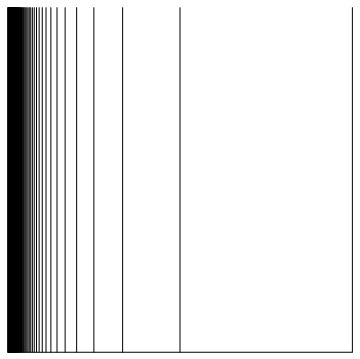
\includegraphics[width=0.28\textwidth]{C:/Users/Nacho/Documents/Latex/Facultad/combspace.png}
	\caption{El peine del topólogo}
	\label{fig:combspace}
\end{figure}

Ahora consideremos $X = C\cup \{(0,1)\}$. Es decir, le agregamos un punto. Notemos que como $C\subseteq X\subseteq \overline{C}$ (donde la clausura la vemos en $X$) y $C$ es conexo (pues en particular es arcoconexo) debemos tener que $X$ es conexo. Pero veamos que $X$ no es arcoconexo. Supongamos que $\gamma:[0,1]\to X$ es tal que $\gamma(0)=(0,1)$ y $\gamma(1)=(1,1)$. $X$ es arcoconexo si y sólo existe ese arco (pues $C$ es arcoconexo y el punto que agregué lo tengo que poder conectar con todos los otros, pero al ser una relación de equivalencia y el resto del espacio arcoconexo, conectarlo con uno es lo mismo que con cualquier otro). Consideremos $f:[0,1]\to\RR$ la función dada por $f(t) = \gamma_2(t) - \gamma_1(t)$ donde $\gamma(t) = (\gamma_1(t),\gamma_2(t))$. Es obvio que $f$ es continua, $f(0)=1$ y $f(1)=0$. Por el teorema de los valores intermedios, existe $\tilde{t}\in (0,1)$ tal que $f(\tilde{t}) = \frac{1}{2}$. Como $\{t\in [0,1] : f(t)=\frac{1}{2}\}$ es no vacío y acotado inferiormente, podemos considerar su ínfimo $t_0$. Como a su vez, ese conjunto es cerrado (por ser la preimagen de $\{\frac{1}{2}\}$ por $f$ que es continua), tenemos que $t_0$ está en el conjunto (pues tiene una sucesión de puntos del conjunto que tienden a él por ser ínfimo y está por ser cerrado el conjunto). Entonces, $f(t_0)=\frac{1}{2}$. Esto quiere decir que $f(t)>\frac{1}{2}$ para todo $t\in [0,t_0)$. Sea $t_1\in [0,t_0)$. Tenemos que $\gamma([0,t_1])$ es conexo y $(0,1)\in \gamma([0,t_1])\subseteq X\cap \{(x,y)\in\RR^2 : y-x>\frac{1}{2}\}\subseteq \QQ\times \RR$. Si $\gamma(t_1)\neq (0,1)$ entonces $\gamma(t_1)=(a,b)$ con $a\in\QQ$, $a>0$. Sea $y\in\RR-\QQ$ con $0<y<a$. Entonces, $U = X\cap ((-\infty,y)\times \RR)$ y $V=X\cap ((y,+\infty)\times \RR)$ desconectan a $\gamma([0,t_1])$. Por lo tanto, $\gamma(t_1)=(0,1)$ para todo $t_1\in [0,t_0)$. Pero $f(t_0) = \frac{1}{2} = \lim_{t\to t_0} f(t) = 1$. Absurdo.

\end{ex}

\begin{prop}
Sea $X$ un espacio topológico. Si $(A_i)_{i\in I}\subseteq X$ es una familia de arcoconexos con $\displaystyle\bigcap_{i\in I}A_i\neq\emptyset$, entonces $\displaystyle\bigcup_{i\in I}A_i$ es arcoconexo.
\begin{proof}
Supongamos que $x,y\in \displaystyle\bigcup_{i\in I}A_i$. Entonces, existen dos índices $j_1,j_2\in I$ tales que $x\in A_{j_1}, y\in A_{j_2}$. Si $a\in \displaystyle\bigcap_{i\in I}A_i$ entonces como $A_{j_1}$ es arcoconexo, tengo que $x$ y $a$ están arcoconectados y como $A_{j_2}$ es arcoconexo tengo que $a$ e $y$ están arcoconectados. Como la relación es transitiva, $x$ e $y$ están arcoconectados y listo.
\end{proof}
\end{prop}

\begin{prop}
Sea $X$ un espacio topológico y $(A_i)_{i\in\NN}$ una sucesión de arcoconexos. Si $A_n\cap A_{n+1}\neq\emptyset$ para cada $n\in\NN$ tenemos que $\displaystyle\bigcup_{i\in \NN}A_i$ es arcoconexo.
\begin{proof}
Definimos $B_n = \displaystyle\bigcup_{i=1}^n A_i$. Podemos probar inductivamente que cada $B_n$ es conexo (pues $B_n = B_{n-1}\cup A_n$ que tienen intersección no vacía y son conexos), y como $B_1\subseteq \displaystyle\bigcap_{i\in \NN}B_i$, la intersección es no vacía y por la proposición anterior debe resultar que $\displaystyle\bigcup_{i\in\NN}B_i$ es conexo. Pero $\displaystyle\bigcup_{i\in\NN}A_i = \displaystyle\bigcup_{i\in\NN}B_i$ y listo.
\end{proof}
\end{prop}

\begin{prop}
Sea $X$ un espacio topológico arcoconexo y $f:X\to Y$ una función continua. Entonces $f(X)$ es arcoconexo.
\begin{proof}
Si $a,b\in f(X)$ entonces $a=f(x), b=f(y)$ con $x,y\in X$. Como $X$ es arcoconexo, existe $\gamma:[0,1]\to X$ continua tal que $\gamma(0)=x, \gamma(1)=y$. Pero entonces consideremos el arco $f\circ\gamma:[0,1]\to f(X)$ es continua por ser composición de continuas y $f\circ\gamma(0)=f(x),f\circ\gamma(1)=f(y)$. La proposición sigue.
\end{proof}
\end{prop}

\begin{prop}
Sea $(X_i)_{i\in I}$ una familia de espacios topológicos. $X_i$ es arcoconexo para todo $i\in I$ si y sólo si $X=\displaystyle\prod_{i\in I}X_i$ (provisto de la topología producto) es arcoconexo.
\begin{proof}
$(\Longleftarrow)$ Es obvio pues $X_i = \pi_i(X)$ que es arcoconexo por ser $\pi_i$ continua y la proposición anterior.

$(\Longrightarrow)$ Sean $x=(x_i)_{i\in I}, y = (y_i)_{i\in I}$ con $x_i,y_i\in X_i$ para cada $i\in I$. Como cada $X_i$ es arcoconexo, existe $\gamma_i:[0,1]\to X_i$ continua tal que $\gamma_i(0)=x_i, \gamma_i(1)=y_i$. Defino entonces $\gamma(t) = (\gamma_i(t))_{i\in I}$. Por la propiedad universal de la topología inicial, como $\pi_i\circ\gamma = \gamma_i$ es continua para cada $i\in I$, resulta que $\gamma$ es continua y listo.
\end{proof}
\end{prop}

\begin{defn}
Sea $X$ un espacio topológico. $A\subseteq X$ es una \textbf{componente arcoconexa} de $X$ si es un subconjunto conexo maximal (es decir, si $A\subseteq B$ con $B$ arcoconexo, entonces $A=B$).
\end{defn}

\begin{prop}
Podemos escribir $X=\displaystyle\bigsqcup_{i\in I}A_i$ con $A_i$ las componentes arcoconexas.
\begin{proof}
Es totalmente análoga a la demostración para las componentes conexas.
\end{proof}
\end{prop}

\begin{obs}
Como cada componente arcoconexa es conexa, está metida en una componente conexa. Entonces, cada componente conexa se parte como unión disjunta de componentes arcoconexas.
\end{obs}

\begin{obs}
No vale que cada componente arcoconexa sea necesariamente cerrada. El ejemplo ya lo vimos y es el del peine del topólogo.
\end{obs}

\begin{defn}
Sea $X$ un espacio topológico. Decimos que $X$ es \textbf{localmente (arco)conexo en $x\in X$} si para todo $U$ abierto, $U\subseteq X$ con $x\in U$, existe un abierto (arco)conexo $V_x$ tal que $x\in V_x\subseteq U$. El espacio $X$ se dice \textbf{localmente (arco)conexo} si es localmente (arco)conexo para todo $x\in X$.
\end{defn}

\begin{ex} Veamos un par de ejemplos:
\begin{itemize}
\item $\RR$ es conexo y localmente conexo.
\item $\RR-\{0\}$ no es conexo pero sí localmente conexo.
\item El peine del topólogo es conexo pero no localmente conexo.
\item $\QQ$ no es conexo ni localmente conexo
\end{itemize}
Todos estos mismos ejemplos sirven si cambiamos conexo por arcoconexo y localmente conexo por localmente arcoconexo.
\end{ex}

\begin{obs}
$X$ es localmente conexo si y sólo si tiene una base formada por abiertos conexos. De la misma forma, $X$ es localmente arcoconexo si tiene una base formada por abiertos arcoconexos.
\end{obs}

\begin{prop}
Sea $X$ un espacio topológico. $X$ es localmente conexo si y sólo si para todo $U\subseteq X$ abierto las componentes conexas de $U$ son abiertas en $X$ (o equivalentemente en $U$).
\begin{proof}
$(\Longrightarrow)$ Sea $C$ una componente conexa de $U$. Si $x\in C\subseteq U$, existe $V_x$ abierto conexo tal que $x\in V_x\subseteq U$. Como $V_x$ es conexo, está en la componente, $V_x\subseteq C$. Entonces, $C=\displaystyle\bigcup_{x\in C}V_x$ es una unión de abiertos y así es abierto.

$(\Longleftarrow)$ Sea $U$ abierto, $x\in U$. Sea $C$ la componente conexa de $U$ que tiene a $x$. Entonces $x\in C\subseteq U$ y así $X$ es localmente conexo.
\end{proof}
\end{prop}

\begin{prop}
Sea $X$ localmente arcoconexo. Entonces, cada componente conexa de $X$ es una componente arcoconexa de $X$.
\begin{proof}
Sea $C$ una componente conexa. Luego, podemos escribir (en virtud de una observación anterior) $C=\displaystyle\bigsqcup_{i\in I}C_i$ donde $C_i$ son componentes arcoconexas de $X$. Cada $C_i$ es un abierto de $X$ por la proposición anterior. Si $\sharp I > 1$ entonces, tomo $i_0\in I$ y considero los abiertos $U=C_{i_0}$, $V=\displaystyle\bigsqcup_{i\in I -\{i_0\}} C_i$ son abiertos disjuntos que desconectan a $C$. Absurdo, por lo tanto $C$ es una componente arcoconexa y listo.
\end{proof}
\end{prop}

\section{Axiomas de Separabilidad}

\begin{defn}
Sea $X$ un espacio topológico. Decimos que $X$ es \textbf{regular} si para todo $x\in X$ y $F\subseteq X$ cerrado tal que $x\in F$, existen dos abiertos $U,V$ disjuntos tales que $x\in U$, $F\subseteq V$.
\end{defn}

\begin{defn}
Sea $X$ un espacio topológico. Decimos que $X$ es \textbf{normal} si para todos cerrados $F_1,F_2\subseteq X$ disjuntos existen abiertos $U,V$ disjuntos con $F_1\subseteq U$, $F_2\subseteq V$.
\end{defn}

\begin{obs}
Que un espacio sea normal no implica que sea regular. Por ejemplo, el Espacio de Sierpinski es normal pero no regular. Un ejemplo similar es $X=\{a,b,c\}$ con $\tau = \{\emptyset, \{a\}, \{a,b\}, \{c\}, \{a,c\},X\}$. La vuelta tampoco es cierta (es decir, regular no implica normal) pero el contraejemplo lo veremos más adelante.
\end{obs}

\begin{defn}
Sea $X$ un espacio topológico.
\begin{itemize}\item Decimos que $X$ es $\mathrm{T}_0$ si para todos los $x,y\in X$ con $x\neq y$ existe un abierto $U$ tal que tiene a uno de $\{x,y\}$ pero no al otro.
\item Decimos que $X$ es $\mathrm{T}_1$ si para todos los $x,y\in X$ con $x\neq y$ existen $U,V$ abiertos tales que $x\in U, y\notin U, x\notin V, y\in V$.
\item Decimos que $X$ es $\mathrm{T}_2$ (o Hausdorff) si para todos los $x,y\in X$ con $x\neq y$ existen abiertos $U,V$ disjuntos tales que $x\in U$, $y\in V$.
\item Decimos que $X$ es $\mathrm{T}_3$ si es $\mathrm{T}_1$ y regular.
\item Decimos que $X$ es $\mathrm{T}_4$ si es $\mathrm{T}_1$ y normal.
\end{itemize}
\end{defn}

\begin{lem}
$X$ es $\mathrm{T}_1$ si y sólo si para todo $x\in X$ tenemos que $\{x\}$ es cerrado.
\begin{proof}
$(\Longrightarrow)$ Sea $x\in X$. Para todo $y\neq x$ existe $V_y$ abierto de $X$ tal que $y\in V_y$ pero $x\notin V_y$. Entonces, $X-\{x\} = \displaystyle\bigcup_{y\in Y}V_y$ es abierto por ser unión de abiertos. Por lo tanto $\{x\}$ es cerrado.

$(\Longleftarrow)$ Simplemente notemos que $U = \{y\}^c$ y $V = \{x\}^c$ son abiertos y por definición tenemos que $x\in U, y\notin U, x\notin V, y\in V$.
\end{proof}
\end{lem}

\begin{cor}
Si $X$ es un espacio topológico vale la cadena de implicaciones $$\mathrm{T}_4\Longrightarrow \mathrm{T}_3 \Longrightarrow \mathrm{T}_2\Longrightarrow \mathrm{T}_1\Longrightarrow \mathrm{T}_0$$
\end{cor}

\begin{ex}
Notemos que si $X=\{a,b,c\}$ con $\tau = \{\emptyset, \{a\},\{b,c\},X\}$ no es $\mathrm{T}_1$ (ni siquiera es $\mathrm{T}_0$) pero es normal y regular.

Sea $X=\NN$ con la topología cofinita. $X$ es $\mathrm{T}_1$. Pero, para todos $U,V$ abiertos no vacíos su intersección es no vacía (es más, hay infinitos puntos en la intersección). Esto quiere decir que $X$ no es normal ni regular. Además, es $\mathrm{T}_1$ pero no $\mathrm{T}_2$.

Otro ejemplo es $\RR^n$ con la topología de Zariski. Si $p=(p_1,\ldots , p_n)$ y $q=(q_1,\ldots , q_n)$ con $p\neq q$ entonces existe un $i$ tal que $p_i\neq q_i$. Consideremos $U = \{x_i = q_i\}^c$ y $V=\{x_i = p_i\}^c$. Son abiertos por definición y $p\in U, q\in V$. Eso quiere decir que es $\mathrm{T}_1$. Ahora bien, veamos que no es $\mathrm{T}_2$. Para eso, veamos que si $U,V$ sob abiertos no vacíos entonces $U\cap V\neq \emptyset$. Si $U=F_{S_1}^c$, $V=F_{S_2}^c$ con $S_1,S_2\subseteq \RR[x_1,\ldots , x_n]$ y $F_S=\{x\in\RR^n : f(x) = 0\;\forall f\in S\}$. Como $U,V\neq \emptyset$ tenemos que $F_{S_1},F_{S_2}\neq\RR^n$ y así existen $f,g\neq 0$ con $f\in S_1, g\in S_2$. Por lo tanto, $fg\neq 0$ y como $\RR$ es infinito, existe un $z\in\RR^n$ tal que $fg(z)\neq 0$. Pero entonces $f(z)\neq 0$ y $g(z)\neq 0$. Es decir, $z\in U\cap V$.

Consideremos $X=\RR$ con la topología que tiene por base: $$\{(a,b) : a,b\in\RR, a<b\} \cup \{(a,b)\cap K^c : a,b\in\RR\}$$ donde $K=\{\frac{1}{n}:n\in\NN\}$. Es muy fácil verificar que esto es una base. Notemos que $K$ es cerrado en esta topología pues $K^c = K^c \cap \RR = K^c \cap \left(\displaystyle\bigcup_{n\in\NN} (-n,n)\right) = \bigcup_{n\in\NN} (-n,n)\cap K^c$ que es unión de abiertos y así abierto. Además, es obvio que este espacio es $\mathrm{T}_2$ pues puedo separar sólo con abiertos de la forma $(a,b)$. Para ver que no es $\mathrm{T}_3$ veamos que no existen dos abiertos disjuntos $U,V$ tales que $0\in U$ y $K\subseteq V$. Supongamos que sí. Como $0\in U$, existe un abierto $\tilde{U}$ de la base tal que $0\in \tilde{U}\subseteq U$ y necesariamente como $\tilde{U}\cap K = \emptyset$ tenemos que $\tilde{U} = (a,b)\cap K^c$ para ciertos $a,b\in\RR$ con $a<b$. Además, existe $n_0\in\NN$ tal que $\frac{1}{n_0}<b$ y un abierto $\tilde{V}$ de la base tal que $\frac{1}{n_0}\in\tilde{V}\subseteq V$. Como $\frac{1}{n_0}\in\tilde{V}$, no puede ser que $\tilde{V} = (c,d)\cap K^c$. Entonces, $\tilde{V} = (c,d)$ para ciertos $c,d\in\RR$, $c<d$. Es fácil ver que $\dfrac{\max\{c,\frac{1}{n_0 + 1}\}+\frac{1}{n_0}}{2} \in \tilde{U}\cap\tilde{V} = \emptyset$. Esto es un absurdo, que vino de suponer que el espacio era $\mathrm{T}_3$.

Si $(X,d)$ es un espacio métrico, entonces es $\mathrm{T}_4$. En efecto, es obvio que $X$ es $\mathrm{T}_1$ (es más, es igual de fácil ver que $X$ es $\mathrm{T}_2$). Ahora, para ver que es normal, sean $F_1,F_2$ cerrados disjuntos. Consideremos $f:X\to\RR$ dada por $f(x)=\dfrac{d(x,F_1)}{d(x,F_1)+d(x,F_2)}$. Como el denominador es $0$ si y sólo si $d(x,F_1)=d(x,F_2)=0$ y eso pasa si y sólo si $x\in F_1\cap F_2 = \emptyset$. Entonces, como $f$ es cociente de continuas con denominador no nulo, es continua. Ahora, si $x\in F_1$ tenemos $f(x)=0$ y si $x\in F_2$ tenemos $f(x)=1$. Consideramos entonces $U=f^{-1}((-\infty,\frac{1}{2}))$ y $V=f^{-1}((\frac{1}{2},+\infty))$. Es claro que $F_1\subseteq U, F_2\subseteq V$ y $U\cap V = \emptyset$.

Si $X$ es un conjunto bien ordenado provisto de la topología del orden, entonces es $\mathrm{T}_4$ (más generalmente, no hace falta pedir bien ordenado, alcanza con totalmente ordenado pero la demostración es más dificil). Notemos que para todos $x,y\in X$ con $x<y$ el conjunto $(x,y]$ es abierto. Hay que ver dos casos: si $y\geq z$ para todo $z\in X$ entonces $(x,y] = (x,+\infty)$ y así es abierto por definición. Si no, existe $z_0\in X$ tal que $y<z_0$. Entonces, $Z=\{z\in X : z>y\}$ es no vacío y así tiene elemento mínimo $z_1$. Entonces, $(x,y] = (x,z_1)$. De manera análoga, tenemos que $(-\infty,y]$ es abierto. Primero veamos que el espacio es $\mathrm{T}_1$. En efecto, si $x\neq y$ con $x<y$ entonces $U = (-\infty,y)$ y $V=(x,+\infty)$ son abiertos que los separan. Ahora, veamos que es normal. Para eso, sean $A,B$ cerrados disjuntos. Para cada $a\in A$, $a\in B^c$, que es abierto. Entonces, existe $I_a$ intervalo tal que $a\in I_a\subseteq B^c$. Además, podemos suponer que $I_a = (x_a,a]$ con $x_a\in X\cup\{-\infty\}$. Ahora, para cada $b\in B$ existe $I_b$ tal que $b\in I_b\subseteq A^c$ con $I_n = [b,y_b)$ con $y_b \in X\cup\{+\infty\}$. Sean $U=\displaystyle\bigcup_{a\in A} I_a$ y $V=\displaystyle\bigcup_{b\in B} I_b$ con $A\subseteq U$ y $B\subseteq V$ y son abiertos por ser uniones de abiertos. Además, son disjuntos. Si no, existirían $z\in X,\,a\in A,\,b\in B$ con $z\in [b,y_b) \cap (x_a,a]$. Como $a\neq b$, supongamos $b<a$. Entonces, $x_a < z\leq b < a$ y así $b\in (x_a, a]\subseteq B^c$. Absurdo.
\end{ex}

\begin{prop}
Si $X$ es $\mathrm{T}_0$, entonces $Y\subseteq X$ con topología subespacio también es $\mathrm{T}_0$.
\begin{proof}
Sean $x,y\in Y$. En particular, como $x,y\in X$ que es $\mathrm{T}_0$, existe $U$ abierto tal que $x\in U, y\notin U$. Entonces, simplemente tomamos $U\cap Y$.
\end{proof}
\end{prop}

\begin{prop}
Si $X$ es $\mathrm{T}_1$, entonces $Y\subseteq X$ con topología subespacio también es $\mathrm{T}_1$.
\begin{proof}
Sean $x,y\in Y$. En particular, como $x,y\in X$ que es $\mathrm{T}_2$, existen $U,V$ abiertos tales que $x\in U, y\in V$. Entonces, simplemente tomamos $U\cap Y$ y $V\cap Y$.
\end{proof}
\end{prop}

\begin{prop}
Si $X$ es $\mathrm{T}_2$, entonces $Y\subseteq X$ con topología subespacio también es $\mathrm{T}_2$.
\begin{proof}
Sean $x,y\in Y$. En particular, como $x,y\in X$ que es $\mathrm{T}_2$, existen $U,V$ abiertos disjuntos tales que $x\in U, y\in V$. Entonces, simplemente tomamos $U\cap Y$ y $V\cap Y$.
\end{proof}
\end{prop}

\begin{prop}
Sea $(X_i)_{i\in I}$ una familia de espacios topológicos. Entonces, $X_i$ es $\mathrm{T}_0$ para todo $i\in I$ si y sólo si $\displaystyle\prod_{i\in I}X_i$ es $\mathrm{T}_0$.
\begin{proof}
$(\Longleftarrow)$ Para cada $i\in I$, sea $\mathrm{inc}_{i}:X_i\to \displaystyle\prod_{i\in I}X_i$ que simplemente manda a un $x_i\in X_i$ a $(\mathrm{inc}_i(x_i))_j = \begin{cases} x_i \text{ si }j=i \\ y_j \text{ si } j\neq i\end{cases}$ donde $y_j\in X_j$ es una constante arbitraria para cada $j\in I$. Esto nos dice que como $X_i$ es homeomorfo con la imagen $\mathrm{inc}_i(X_i)$, que es un subespacio de $\displaystyle\prod_{i\in I}X_i$, debe ser $\mathrm{T}_0$ y listo.

$(\Longrightarrow)$ Sean $x=(x_i)_{i\in I}, y=(y_i)_{i\in I}$ con $x\neq y$. Entonces, existe un $i_0\in I$ tal que $x_{i_0}\neq y_{i_0}$. Entonces, existe un abierto $\tilde{U}$ de $X_{i_0}$ tal que $x_{i_0}\in \tilde{U}, y_{i_0}\notin \tilde{U}$. Consideremos $U=\pi_{i_0}^{-1}(\tilde{U})$ abierto del producto (por ser las proyecciones continuas) y además $x\in U$ pero $y\notin U$. Y listo.
\end{proof}
\end{prop}

\begin{obs}
Con exactamente la misma demostración que en la proposición anterior, podemos probar que una familia de espacios topológicos son todos $\mathrm{T}_1$ si y sólo si el producto es $\mathrm{T}_1$ y son todos $\mathrm{T}_2$ si y sólo si el producto es $\mathrm{T}_2$.
\end{obs}

\begin{prop}
Sea $X$ un espacio topológico $\mathrm{T}_2$ y $\alpha:\Gamma\to X$ una red. Si $(x_\alpha)_{\alpha\in\Gamma}$ tiende a $x$ y tiende a $y$, entonces $x=y$. Es decir, los límites son únicos.
\begin{proof}
Si $x\neq y$ entonces existen $U,V$ abiertos disjuntos con $x\in U, y\in V$. Como $x_\alpha\to x$, existe $\alpha_0\in\Gamma$ tal que si $\alpha\geq \alpha_0$ entonces $x_\alpha\in U$. Además, como $x_\alpha\to y$, existe $\alpha_1\in\Gamma$ tal que si $\alpha\geq\alpha_1$ entonces $x_\alpha\in V$. Pero como $\Gamma$ es un conjunto dirigido, existe $\alpha_2\in\Gamma$ tal que $\alpha_2\geq \alpha_0,\alpha_1$. Pero esto implica que si $\alpha\geq \alpha_2$ entonces $x_\alpha \in U\cap V$. Absurdo.
\end{proof}
\end{prop}

\begin{prop}
Sea $X$ un espacio topológico y $\Delta = \{(x,x) : x\in X\}\subseteq X\times X$ la diagonal (con topología producto). Entonces, son equivalentes:
\begin{enumerate}
\item $X$ es $\mathrm{T}_2$.
\item $\Delta$ es cerrado.
\end{enumerate}
\begin{proof}
$(1)\Longrightarrow (2)$: Veamos que $\Delta^c$ es abierto. Sea $(x,y)\in\Delta^c$, es decir, $x\neq y$. Como $X$ es $\mathrm{T}_2$, existen abiertos disjuntos $U_{x,y}, V_{x,y}$ tales que $x\in U_{x,y}, y\in V_{x,y}$. La condición de que sean disjuntos se traduce como que $(U_{x,y}\times V_{x,y})\cap \Delta = \emptyset$. Es decir, $\Delta^c = \displaystyle\bigcup_{(x,y)\in\Delta^c} U_{x,y}\cap V_{x,y}$, que es una unión de abiertos y así abierto.

$(2)\Longrightarrow (1)$: Sea $x\neq y$. Entonces, $(x,y)\in \Delta^c$, que es abierto. Es decir, existen $U,V$ abiertos en $X$ tales que $(x,y)\in U\times V\subseteq \Delta^c$. Pero esto es, $x\in U, y\in V$ y $U\cap V=\emptyset$. Y listo.
\end{proof}
\end{prop}

\begin{lem}
Sean $f,g:Y\to X$ dos funciones continuas con $X$ un espacio $\mathrm{T}_2$. Entonces, $\{y\in Y : f(y)=g(y)\}$ es cerrado.
\begin{proof}
Notemos que $h:Y\to X\times X$ definida por $h(y) = (f(y),g(y))$ es continua por la propiedad universal de la topología producto. Entonces, $\{y\in Y : f(y)=g(y)\} = h^{-1}(\Delta)$, que es cerrado por ser preimagen de un cerrado por una función continua. El lema sigue.
\end{proof}
\end{lem}

\begin{prop}
Si $f,g:Y\to X$ son funciones continuas, $X$ es $\mathrm{T}_2$ y $A\subseteq Y$ es un denso tal que $f(y)=g(y)$ para todo $y\in A$, entonces $f=g$.
\begin{proof}
Simplemente es notar que $A\subseteq \{y\in Y : f(y)=g(y)\}$, que es cerrado por el lema anterior y así contiene a la clausura de $A$. Pero eso es todo $Y$ por ser $A$ denso. Es decir, $Y = \{y\in Y : f(y)=g(y)\}$ y así $f=g$. Como queríamos probar.
\end{proof}
\end{prop}

\begin{teo}
Sea $X$ un espacio topológico regular que admite una base numerable. Entonces, $X$ es normal.
\begin{proof}
Sean $A,B\subseteq X$ cerrados disjuntos. Para cada $x\in A$, existen $\tilde{U}_x, \tilde{V}_x$ abiertos tales que $x\in \tilde{U}_x$, $B\subseteq \tilde{V}_x$ y $\tilde{U}_x\cap\tilde{V}_x = \emptyset$. Sea $\mathscr{B}$ una base numerable de abiertos de $X$. Existe $U_x\in\mathscr{B}$ tal que $x\in U_x\subseteq \tilde{U}_x$. Pero como $U_x\subseteq \tilde{V}_x^c$, tenemos que $\overline{U_x}\subseteq \tilde{V}_x^c$ por ser $\tilde{V}_x^c$ cerrado. Entonces, $\overline{U}_x\cap B = \emptyset$. De forma análoga, para cada $y\in B$ exoste $V_y\in\mathscr{B}$ abierto con $y\in V_y$ y $\overline{V}_y\cap A = \emptyset$. Como $\{U_x\}_{x\in A}\subseteq \mathscr{B}$, debe ser numerable. Entonces, sea $\{U_n\}_{n\in\NN}$ una enumeración de $\{U_x\}_{x\in A}$. De la misma forma, sea $\{V_n\}_{n\in\NN}$ una enumeración de $\{V_y\}_{y\in B}$. Consideremos entonces $\hat{U} = \displaystyle\bigcup_{n\in\NN} U_n$ y $\hat{V} = \displaystyle\bigcup_{n\in\NN} V_n$. Es claro que son abiertos pues son uniones de abiertos. Además, $A\subseteq\hat{U}$ y $B\subseteq\hat{V}$. También sabemos que $A\cap\hat{V}=\emptyset$ pues $A\cap V_n=\emptyset$ para todo $n\in\NN$. Por la misma razón, $B\cap\hat{U} = \emptyset$. 

Vamos a definir $\tilde{U}_n = U_n \cap \left(\displaystyle\bigcap_{i=1}^n \overline{V}_i^c\right)$ y $\tilde{V}_n = V_n \cap \left(\displaystyle\bigcap_{i=1}^n \overline{U}_i^c\right)$. Son abiertos por ser intersecciones finitas de abiertos. Tomemos entonces $U=\displaystyle\bigcup_{n\in\NN}\tilde{U}_n$ y $V = \displaystyle\bigcup_{n\in\NN}\tilde{V}_n$. Estos abiertos nos van a servir. En efecto, $A\subseteq U, B\subseteq V$ (pues si $a\in A$ existe $n_0$ tal que $a\in U_{n_0}$ pero $\overline{V}_{n_0}\cap A = \emptyset$).

Quiero ver que $U\cap V = \emptyset$. Sea $z\in U\cap V$. Entonces, existen $k,\ell$ tales que $z\in \tilde{U}_k\cap \tilde{V}_\ell$. Sin pérdida de la generalidad, $k\geq \ell$. Pero tenemos que $z\in \tilde{U}_k = U_k \cap \left(\displaystyle\bigcap_{i=1}^k \overline{V}_k^c\right)\subseteq V_\ell^c$ y $z\in \tilde{V}_\ell = V_l \cap \left(\displaystyle\bigcap_{i=1}^\ell \overline{U}_i^c\right) \subseteq V_\ell$. Absurdo.
\end{proof}
\end{teo}

\begin{prop}
Sea $X$ regular, $Y\subseteq X$ un subespacio. Entonces $Y$ es regular.
\begin{proof}
Sea $F\subseteq Y$ cerrado en $Y$ y sea $y\in Y$, $y\notin F$. Entonces, existe $\tilde{F}$ cerrado en $X$ tal que $F=\tilde{F}\cap Y$, con $y\notin \tilde{F}$ (pues si estuviera en $\tilde{F}$, como está en $Y$ estaría en la intersección, que es $F$). Como $X$ es regular, existen abiertos $U,V$ de $X$ tales que $y\in U$, $\tilde{F}\subseteq V$ y $U\cap V=\emptyset$. Tomo entonces $U\cap Y$ y $V\cap Y$, y listo.
\end{proof}
\end{prop}

\begin{cor}
Si $X$ es $\mathrm{T}_3$, entonces $Y\subseteq X$ con topología subespacio también es $\mathrm{T}_3$.
\begin{proof}
Simplemente es notar que la propiedad vale para $\mathrm{T}_1$ y para normal.
\end{proof}
\end{cor}

\begin{prop}
Sea $(X_i)_{i\in I}$ una familia de espacios topológicos. $X_i$ es regular para todo $i\in I$ si y sólo si $\displaystyle\prod_{i\in I}X_i$ es regular.
\begin{proof}
$(\Longleftarrow)$ Es la misma idea que antes, vemos a cada $X_i$ como un subespacio del producto vía la inclusión y nos queda que es regular por ser subespacio de un regular.

$(\Longrightarrow)$ Sea $x=(x_i)_{i\in I}$ y $F$ cerrado (no vacío) con $x\notin F$. Entonces, $x\in F^c$ que es abierto. Esto implica que existe un abierto $X'$ de la base tal que $x\in X'\subseteq F^c$. Por lo tanto, $X' = \displaystyle\prod_{i\in I} X_i'$ con $X_i'$ abierto de $X_i$ y $I' = \{i\in I : X_i'\neq X_i\}$ finito. Para cada $i\in I'$, $x_i\in X_i'$, y así $x_i\notin X_i'^c$, que es cerrado. Como cada espacio es regular, existen $U_i,V_i$ abiertos de $X_i$ con $x\in U_i$, $X_i'^c\subseteq V_i$ y $U_i\cap V_i = \emptyset$. Ahora simplemente defino $U = \displaystyle\bigcap_{i\in I'} \pi_i^{-1}(U_i)$ y $V=\displaystyle\bigcap_{i\in I'} \pi_i^{-1}(V_i)$ que son abiertos por ser intersecciones finitas de abiertos. Es claro que $x\in U$ pues $x_i\in U_i$ para cada $i\in I'$. También es claro que $F\subseteq V$ pues $F\subseteq X'^c$ y $X'^c\subseteq V$. Resta ver que $U\cap V = \emptyset$. Pero si $z = (z_i)_{i\in I} \in U\cap V$, existe $i_0\in I'$ tal que $z\in \pi_{i_0}^{-1}(V_{i_0})$. Esto quiere decir que $z_{i_0}\in V_{i_0}$, y de la misma forma $z_{i_0}\in U_{i_0}$. Absurdo. 
\end{proof}
\end{prop}

\begin{obs}
Notemos que productos de espacios normales no necesariamente son normales. En efecto, veamos un ejemplo. Sea $X$ totalmente ordenado. Decimos que $I\subseteq X$ es \textbf{sección} si $\forall x\in X$, $y\in I$ tenemos que $x<y$ implica que $x\in I$. Sea $X$ un conjunto no numerable y bien ordenado. Definimos $Y=\{1,2\}\times  X$ ordenado vía $(a,x)\leq (a',x')$ por $a<a'$ ó $a=a'$ y $x\leq x'$ (es decir, el orden lexicográfico). $Y$ resulta bien ordenado. Sea $x_0\in X$ el primer elemento de $X$. Entonces, $(-\infty, (2,x_0))$ es una sección propia no numerable.

Consideremos $Z=\{\alpha\in Y : \sharp(-\infty, \alpha)>\aleph_0\}$. Es claro que $Z\neq\emptyset$ pues en el párrafo anterior construimos una sección propia no numerable. Ahora, sea $\Omega$ el primer elemento de $Z$ y $S=(-\infty,\Omega)$. Es fácil ver que su clausura es $\overline{S} = (-\infty, \Omega]$. Notemos que $S$ no tiene elemento máximo. Si lo tuviera, lo llamamos $a$ y entonces, $S=(-\infty,a)\cup \{a\}$ es numerable. Absurdo, pues $S=(-\infty,\Omega)$ que es una sección no numerable.

Como $S$ y $\overline{S}$ son bien ordenados, sabemos que deben ser normales. Pero veamos entonces que $S\times\overline{S}$ no es normal. Notemos primero que en $S\times \overline{S}$ coinciden la topología producto con la topología subespacio en $\overline{S}\times\overline{S}$.

Sean $A=\{(x,x) : x\in S\}$ y $B=\{(x,\Omega):x\in S\}$. Consideremos $\Delta = \{(x,x) : x\in\overline{S}\}$ la diagonal de $\overline{S}\times\overline{S}$. Como $\overline{S}$ es $\mathrm{T}_2$, tenemos que $\Delta$ es cerrado. Entonces, $A=\Delta\cap (S\times\overline{S})$ es cerrado. Ahora, $B^c = S\times S$, que es abierto pues $S\subseteq\overline{S}$ es abierto. Supongamos que $U,V$ son abiertos disjuntos tales que $A\subseteq U$ y $B\subseteq V$. Para cada $x\in S$, consideremos el conjunto $A_x = \{y\in S : x<y, (x,y)\notin U\}$. Veamos que $A_x\neq\emptyset$. Sea $(x,\Omega)\in B\subseteq V$. Existen $W_1\subseteq S,\; W_2\subseteq \overline{S}$ abiertos tales que $(x,\Omega)\in W_1\times W_2 \subseteq V$, y así $\Omega\in W_2$. Entonces, existe $a\in S$ tal que $\Omega\in (a,\Omega]\subseteq W_2$. Como $S$ no tiene elemento máximo, existe $a'\in (a,\Omega]$. Además, $a>x$ pues si $a\leq x$ entonces $(x,x)\in W_1\times W_2$. Luego, $(x,a')\in V$.

Para cada $x\in S$, sea $\beta(x)$ el primer elemento de $A_x$. Sea $x_1\in S$ cualquiera. Consideremos la sucesión definida por $x_{n+1}=\beta(x_n)$. La sucesión $(x_n)_{n\in\NN}$ es acotada en $S$. En efecto, si no lo fuera, $S = \displaystyle\bigcup_{n\in\NN} \{x\in S : x< x_n\}$ tendríamos que $S$ es numerable pues cada $\{x\in S : x< x_n\}$ es numerable por ser una sección propia. Entonces, $(x_n)_{n\in\NN}$ es acotada. Sea $b\in S$ el primer elemento de $\{b'\in S : x_n \leq b' \;\forall n\in\NN\}$. Entonces, $(b,b)\in A\subseteq U$. Esto quiere decir que existen $b_1,b_2\in B$ tales que $(b,b)\in (b_1,b_2)\times (b_1,b_2)\subseteq U$. Como $b_1$ no es cota superior (pues $b_1<b$) existe un $n_0\in\NN$ tal que $b_1< x_{n_0}<x_{n_0+1}\leq b<b_2$. Es decir, $(x_{n_0},x_{n_0+1}) = (x_{n_0},\beta(x_{n_0})) \in (b_1,b_2)\times(b_1,b_2)\subseteq U$. Absurdo, pues $(x,\beta(x))\notin U$ para todo $x\in S$. Este absurdo vino de suponer que existen abiertos disjuntos que separan a $A$ y $B$. Por lo tanto, $S\times\overline{S}$ no es normal.

Esto nos provee a su vez de un ejemplo de que subespacio de normal no necesariamente es normal, pues $S\times\overline{S}\subseteq \overline{S}\times\overline{S}$ no es normal mientras que $\overline{S}\times\overline{S}$ sí lo es (aunque la demostración la veremos luego).

\end{obs}

\begin{lem}[Lema de Urysohn]
Sea $X$ un espacio topológico normal y $A,B$ cerrados disjuntos. Entonces, existe una función continua $f:X\to [0,1]$ tal que $f(x)=0$ para todo $x\in A$ y $f(x)=1$ para todo $x\in B$.
\begin{proof}
Sean $U,V$ abiertos disjuntos tales que $A\subseteq U$ y $B\subseteq V$. Como son disjuntos tenemos $U\subseteq V^c$. Entonces, $\overline{U}\subseteq V^c$ (pues $V^c$ es un cerrado que contiene a $U$ y así a su clausura). Luego, $\overline{U}\subseteq V^c \subseteq B^c$. Vamos a definir, para cada $p\in\QQ$ un abierto $U_p$ de modo tal que si para $p_1,p_2\in\QQ$ con $p_1<p_2$ entonces $\overline{U_{p_1}}\subseteq U_{p_2}$.

Consideremos los abiertos definidos por $$U_p = \begin{cases} \emptyset \text{ si }p<0 \\ U \text{ si }p=0 \\ B^c \text{ si }p=1 \\ X \text{ si }p>1\end{cases}$$ Ahora, definamoslos en $\QQ\cap (0,1)$. Sea $\varphi:\NN\to \QQ\cap (0,1)$ una biyección (que existe por cardinalidad) y supongamos que tenemos definidos $U_{\varphi(1)},\ldots , U_{\varphi(k)}$ que satisfacen lo que buscamos. Vamos a construirnos $U_{\varphi(k+1)}$. Sean $p_1 = \max(\{0,\varphi(1),\ldots , \varphi(k)\}\cap [0,\varphi(k+1)))$ y $p_2 = \min(\{1,\varphi(1),\ldots , \varphi(k)\}\cap (\varphi(k+1),1])$. Sabemos que $\overline{U_{p_1}}\subseteq U_{p_2}$. Entonces, $\overline{U_{p_1}}$ y $U_{p_2}^c$ son cerrados disjuntos. Por normalidad, esto implica que existen $W_1,W_2$ abiertos disjuntos con $\overline{U_{p_1}}\subseteq W_1$ y $U_{p_2}^c \subseteq W_2$. Tomemos $U_{\varphi(k+1)} = W_1$. Entonces, $W_1\subseteq V^c$ y así $\overline{W_1}\subseteq V^c\subseteq U_{p_2}$. Es decir, $\overline{U_{p_1}}\subseteq U_{\varphi(k+1)}$ y $\overline{U_{\varphi(k+1)}}\subseteq U_{p_2}$, como queríamos construir.

Para cada $x\in X$, definamos $f(x) = \inf \{p\in\QQ : x\in U_p\}$. Notemos que este conjunto es no vacío pues $(1,+\infty)$ está contenido en él, y además está acotado inferiormente, pues el conjunto está metido en $[0,+\infty)$. Es fácil ver que $f(x)\in [0,1]$, pues si $x\in A$ tenemos que $\{p\in \QQ : x\in U_p\} = [0,+\infty)\cap\QQ$ y así el ínfimo es $0$ y lo análogo para $x\in B$. Además, es obvio ver que $f(x)=0$ si $x\in A$ y $f(x)=1$ si $x\in B$. Resta ver que $f$ es continua.

Para ver que $f$ es continua, basta ver que $f^{-1}([0,a))$ es abierto si $a\in (0,1]$ y $f^{-1}((a,1])$ es abierto si $a\in [0,1)$. Sea $a\in (0,1]$ y sea $x\in f^{-1}([0,a))$. Entonces, $f(x)<a$ y así existe $p_x\in\QQ$ tal que $f(x)<p_x<a$. Esto implica que $x\in U_{p_x}\subseteq f^{-1}([0,a))$, pues por definición, $f(x)=\inf\{p\in\QQ : x\in U_p\}$ y así $x\in U_{f(x)}\subseteq \overline{U_{f(x)}}\subseteq U_{p_x}$. Esto quiere decir que podemos escribir $f^{-1}([0,a)) = \displaystyle\bigcup_{x\in f^{-1}([0,a))} U_{p_x}$ y así es abierto. Ahora, sea $a\in [0,1)$ y sea $x\in f^{-1}((a,1])$. Entonces, $f(x)>a$ y así existen $p_x,p_x'\in\QQ$ con $a<p_x<p_x'<f(x)$. Por lo tanto, $x\notin U_{p_x'}$ y así $x\notin \overline{U_{p_x}}$. Luego, tenemos que $x\in \overline{U_{p_x}}^c\subseteq f^{-1}((a,1])$. En efecto, si $y\in \overline{U_{p_x}}^c$ entonces $y\notin U_{p_x}$ y así $f(y)\geq p_x>a$. Esto nos dice que podemos escribir $f^{-1}((a,1]) = \displaystyle\bigcup_{x\in f^{-1}((a,1])} \overline{U_{p_x}}^c$. Por lo tanto $f$ es continua, como queríamos.

\end{proof}
\end{lem}

\begin{lem}
El espacio $X=\RR^{\NN}$ con topología producto es metrizable.
\begin{proof}
Definamos $\overline{d}:\RR\times\RR\to\RR$ por $\overline{d}(a,b) = \min \{|a-b|,1\}$. Es fácil ver que $\overline{d}$ es una métrica en $\RR$. Definamos $D:\RR^\NN\times\RR^\NN$ por $D((x_i)_{i\in \NN}, (y_i)_{i\in\NN}) = \displaystyle\sup \left\{ \dfrac{\overline{d}(x_i,y_i)}{i} : i\in\NN \right\}$. Es fácil ver que $D$ es una distancia. Veamos que la topología producto de $\RR^\NN$ coincide con la topología inducida por la métrica $D$.

Sea $U$ un abierto en la topología inducida por $D$. Sea $x\in U$. Entonces, existe $\varepsilon>0$ tal que $B(x,\varepsilon)\subseteq U$. Sea $N\in\NN$ tal que $\frac{1}{N}<\varepsilon$. Consideremos entonces el abierto de la topología producto de $\RR^\NN$: $$V=(x_1-\varepsilon,x_1+\varepsilon)\times\ldots \times(x_N-\varepsilon,x_N+\varepsilon)\times\RR\times\ldots$$ Veamos que $V\subseteq U$. En efecto, si $y\in V$ y $1\leq i\leq N$, tenemos que $\dfrac{\overline{d}(x_i,y_i)}{i} \leq\dfrac{\varepsilon}{i}< \varepsilon$ y si $i\geq N+1$ tenemos que $\dfrac{\overline{d}(x_i,y_i)}{i}\leq\dfrac{1}{N+1}<\varepsilon$. Tenemos entonces que $D(x,y)<\varepsilon$. Además, es obvio que $x\in V$. Como $x\in V\subseteq U$, tenemos que $U$ es abierto en la topología producto.

Ahora, sea $U$ un abierto en la topología producto y sea $x\in U$. Tomemos un abierto de la base que contenga a $x$ y esté en $U$. Es decir, sean $U_1,\ldots , U_N$ abiertos de $\RR$ con $$ x\in U_1\times U_2\times\ldots \times U_N \times\RR\times\ldots\subseteq U$$ Entonces, existen $\varepsilon_1,\ldots , \varepsilon_N>0$ tales que $(x_i-\varepsilon_i,x_i+\varepsilon_i)\subseteq U_i$ para todo $1\leq i\leq N$. Podemos suponer sin pérdida de la generalidad que $\varepsilon_i <1$ para todo $1\leq i\leq N$. Sea $\varepsilon = \min\{\frac{\varepsilon_1}{1},\ldots , \frac{\varepsilon_N}{N}\}$ y sea $y\in B(x,\varepsilon)$.  Sabemos que $\dfrac{\overline{d}(x_i,y_i)}{i}<\varepsilon \leq \dfrac{\varepsilon_i}{i}$, y por lo tanto, $\overline{d}(x_i,y_i) < \varepsilon_i < 1$. Esto quiere decir que $|x_i-y_i|<\varepsilon_i$ y así $y_i\in U_i$ para cada $1\leq i \leq N$. Y estamos.
\end{proof}
\end{lem}

\begin{teo}[Teorema de Metrizabilidad de Urysohn]
Cualquier espacio topológico $X$ que admite una base numerable y es $\mathrm{T}_3$ es metrizable.
\begin{proof}
Si $X$ tiene un punto ya estamos. Supongamos entonces $\sharp X>1$. Sabemos que $X$ es regular con una base numerable, y así debe ser normal. Entonces, $X$ es $\mathrm{T}_4$. Sea $\mathscr{B} = \{B_i\}_{i\in\NN}$ una base de la topología en $X$. Consideremos ahora el conjunto de índices $A=\{(i,j)\in\NN\times\NN : \overline{B_i}\subseteq B_j\}$. Notemos que $A$ es no vacío. En efecto, sean $x,y\in X$ con $x\neq y$. Como $X$ es $\mathrm{T}_3$ (y por lo tanto $\mathrm{T}_2$), existen $U,V$ abiertos disjuntos tales que $x\in U, y\in V$. Esto quiere decir que existe $j\in\NN$ tal que $x\in B_j\subseteq U$ con $x\notin B_j^c$. Ahora, existen abiertos $\tilde{U},\tilde{V}$ disjuntos tales que $x\in\tilde{U}$ y $B_j^c\subseteq\tilde{V}$. Luego, existe algún $i\in\NN$ tal que $x\in B_i\subseteq \tilde{U}$, y así como $\tilde{U}\subseteq \tilde{V}^c$, tenemos que $\overline{B_i}\subseteq \tilde{V}^c \subseteq B_j$.

En virtud del Lema de Urysohn, para cada par $(i,j)\in A$ existe $f_{ij}:X\to \RR$ continua tal que $f_{ij}(x) = 1$ para todo $x\in\overline{B_i}$ y $f_{ij}(x)=0$ para todo $x\in B_j^c$. Debemos considerar ahora dos casos:

En el caso que $A$ es infinito, consideremos $F:X\to\RR^\NN$ donde $F(x)= (f_{ij}(x))_{(i,j)\in A}$ (notemos que esto está bien definido porque $(i,j)\in A$ es numerable y así se pueden indexar por los naturales). Veamos que $F$ es un homeomorfismo con su imagen. Esto implicará que, como $\RR^\NN$ es metrizable, es homeomorfo a un subespacio de un metrizable, que lo es con la distancia inducida en el subespacio. Para probar esto, veamos que $F$ es biyectiva, continua y abierta. Es claro que $F$ es inyectiva, pues si $x\neq y$ entonces existen $(i,j)\in A$ tales que $y\notin B_j$ y así $f_{ij}(x)=1$ pero $f_{ij}(y)=0$ (pues los construímos de la misma forma que hicimos para probar que $A$ es no vacío). Por lo tanto en el $(i,j)$-ésimo lugar no coinciden $F(x)$ y $F(y)$. Además, $F$ es obviamente sobreyectiva pues estamos correstringiendonos a su imagen. También es fácil ver que $F$ es continua por la propiedad universal de la topología producto: la composición de $F$ con cada proyección es $f_{ij}$ que son continuas por como las tomamos. Sólo resta ver que es abierta.

Sea $U$ un abierto de $X$ y sea $x\in U$. Quiero ver que $F(x)\subseteq U_x\subseteq F(U)$ para algún $U_x$ abierto. Si $U=X$ es obvio. Si no, existe $(i,j)\in A$ con $x\in B_i$, $\overline{B_i}\subseteq B_j$. Sea $W_x$ el abierto de $\RR^\NN$ que consiste en copias de $\RR$ salvo en el $(i,j)$-ésimo lugar que tiene $(0,+\infty)$. Es claro que $F(x)\subseteq W_x$ pues $f_{ij}(x)=1$ por ser $x\in B_i\subseteq\overline{B_i}$ y no hay nada que verificar en las otras coordenadas. Quiero ver que el abierto $U_x = W_x\cap F(X)$ está incluído en $F(U)$. Sea $z\in F(x')\in W_x$. Si $x'\notin U$, entonces $x'\in U^c$ y así $x'\in B_j^c$. Entonces, $f_{ij}(x')=0$. Pero esto quiere decir que $f(x')\notin W_x$. Absurdo. Por lo tanto, $x'\in U$ y así $z\in F(U)$ y la función es abierta como queríamos.

En el caso que $A$ se finito, hacemos el mismo argumento pero consideramos $F:X\to \RR^n$ con $n=\sharp A$ y notamos que eso es un espacio métrico con la distancia infinito. Y estamos.
\end{proof}
\end{teo}

\begin{defn}
Un espacio topológico $X$ se dice \textbf{completamente regular} si para todo $x\in X$ y $F\subseteq X$ cerrado con $x\notin F$ existe alguna función $f:X\to [0,1]$ continua tal que $f(x)=1$ y $f(y)=0$ para todo $y\in F$.
\end{defn}

\begin{defn}
Un espacio topológico $X$ se dice \textbf{Tychonoff} si es completamente regular y $\mathrm{T}_4$. A los espacios Tychonoff también se les dice $\mathrm{T}_{3,5}$.
\end{defn}

\begin{prop}
Si un espacio topológico $X$ es $\mathrm{T}_4$ entonces es Tychonoff.
\begin{proof}
Sea $x\in X$ y $F\subseteq X$ cerrado con $x\notin F$. Como el espacio es $\mathrm{T}_1$, tenemos que $\{x\}$ es cerrado y así $\{x\}$ y $F$ son cerrados disjuntos. Por el Lema de Urysohn, tengo una función continua que los separa y listo.
\end{proof}
\end{prop}

\begin{prop}
Si un espacio topológico $X$ es completamente regular, entonces es regular.
\begin{proof}
Sea $x\in X$ y $F\subseteq X$ cerrado con $x\notin F$. Sea $f:X\to [0,1]$ continua tal que $f(x)=0$ y $f(y)=1$ para todo $y\in F$. Tomemos entonces $U = f^{-1}([0,\frac{1}{2}))$ y $V=f^{-1}((\frac{1}{2},1])$. Estos abiertos $U,V$ son disjuntos y $x\in U$, $F\subseteq V$. Como queríamos.
\end{proof}
\end{prop}

\begin{cor}
Si $X$ es Tychonoff entonces es $\mathrm{T}_3$.
\end{cor}

\begin{obs}
Notemos que $X$ normal no implica que sea completamente regular. En efecto, el espacio de Sierpinski es un ejemplo. Otro ejemplo levemente más interesante es $X=\{a,b,c\}$ con $\tau=\{\emptyset, \{a\}, \{a,b\}, \{c\}, \{a,c\},X\}$.
\end{obs}

\begin{lem}
Sea $X$ un espacio topológico completamente regular. Si $Y\subseteq X$ es un subespacio, entonces $Y$ es completamente regular.
\begin{proof}
Sea $x\in Y$ y $F\subseteq Y$ cerrado con $x\notin F$. Entonces, existe $F'\subseteq X$ cerrado tal que $F=F'\cap Y$. Además, $x\notin F'$ pues si no tendríamos que $x\in F$. Como $X$ es completamente regular, existe $f: X\to [0,1]$ tal que $f(x)=1$ y $f(y)=0$ para todo $y\in F'$. Es claro que $\left. f\right|_{Y}$ sirve para separar a $x$ de $F$. Y listo.
\end{proof}
\end{lem}

\begin{cor}
Si $X$ es un espacio topológico Tychonoff entonces $Y\subseteq X$ subespacio también es Tychonoff.
\end{cor}

\begin{lem}
Sea $(X_i)_{i\in I}$ una familia de espacios topológicos. Entonces, cada $X_i$ con ${i\in I}$ es completamente regular si y sólo si $\displaystyle\prod_{i\in I}X_i$ es completamente regular.
\begin{proof}
$(\Longleftarrow)$ Podemos mirar a $X_i$ como un subespacio de $\displaystyle\prod_{i\in I}X_i$ incluyéndolo en la $i$-ésima coordenada y dejando todo el resto fijo. Por el lema anterior, subespacio de un completamente regular es completamente regular y listo.

$(\Longrightarrow)$ Sea $x = (x_i)_{i\in I}\in\displaystyle\prod_{i\in I}X_i$ y $F\subseteq \displaystyle\prod_{i\in I}X_i$ cerrado con $x\notin F$. Entonces, $x\in F^c$, que es abierto. Por lo tanto, existe un abierto de la base que contiene a $x$ y que queda contenido en $F^c$. Es decir, $x\in X'\subseteq F^c$ donde $X' = \displaystyle\prod_{i\in I'} X_i'$ con cada $X_i'\subseteq X_i$ abierto y $I' =\{i\in I : X_i' \neq X_i\}$ finito. Para cada $i\in I'$ tenemos $x_i\in X_i'$ y así $x_i\notin X_i'^c$, que es cerrado. Como cada $X_i$ es completamente regular, existen $f_i:X_i\to [0,1]$ continuas tales que $f_i(x_i) = 1$ y $\left. f_i\right|_{X_i'^c} = 0$. Consideramos entonces $f:X\to [0,1]$ dada por $f(x) = \displaystyle\prod_{i\in I'}f_i(x_i)$. Es claramente continua y es obvio que $f(x)=1$. Además, como $F\subseteq X'^c$, si $y\in F$, existe $i_0\in I'$ tal que $y_{i_0}\notin X_{i_0}'$ y así $f_{i_0}(y_{i_0})=0$. Entonces, $f(y)=0$, como queríamos.
\end{proof}
\end{lem}

\begin{obs}
Veamos que Tychonoff no implica $\mathrm{T}_4$. En efecto, si consideramos $S=(-\infty,\Omega)$ como en el ejemplo de "`productos de espacios normales no necesariamente son normales"', ya probamos que $S\times\overline{S}$ no es $\mathrm{T}_4$, pero $S$ y $\overline{S}$ son $\mathrm{T}_4$ y así Tychonoff. Entonces, su producto es Tychonoff pero no $\mathrm{T}_4$.
\end{obs}

\begin{obs}
Veamos que $\mathrm{T}_3$ no implica que el espacio sea Tychonoff.

Para cada entero par $n$, sea $T_n = \{n\}\times (-1,1)$ y sea $X_1 = \displaystyle\bigcup_{n\text{ par}} T_n$. Sea ahora $(t_k)_{k\in\NN}$ una sucesión creciente de reales positivos que converja a $1$. Para cada entero impar, sea $T_n = \displaystyle\bigcup_{k\geq 1}\{(x,y)\in\RR^2 : (x-n)^2 + y^2 = t_k^2\}$ y sea $X_2 = \displaystyle\bigcup_{n\text{ impar}}T_n$. Definamos entonces $X= \displaystyle\bigcup_{n\in\NN}T_n \cup \{a,b\}$. Vamos a darle una topología a $X$ tomando por base a:
\begin{itemize}
\item Todo punto de $X_2$ es aislado excepto los puntos $(n,t_k)$.
\item Un entorno de $(n,t_k)$ consiste de todos los elementos, salvo finitos, de $\{(x,y)\in\RR^2 : (x-n)^2 + y^2 = t_k^2\}$.
\item Un entorno de un punto $(n,y)\in X_1$ consiste de todos los elementos, salvo finitos de $\{(z,y) : n-1 < z < n+1\}\cap (T_{n-1}\cup T_n)$.
\item Un entorno de $a$ es un conjunto $U_c$ que contiene a $a$ y todos los puntos de $X_1\cup X_2$ con primera coordenada mayor que $c$.
\item Un entorno de $b$ es un conjunto $V_d$ que contiene a $b$ y todos los puntos de $X_1\cup X_2$ con primera coordenada menor que $d$.
\end{itemize}

Es fácil chequear que $X$ es $\mathrm{T}_1$ y regular. Es decir, que es $\mathrm{T}_3$. Ahora bien, si fuera completamente regular existiría $f:X\to [0,1]$ continua con $f(a)=0$ y $f(b)=1$. Pero si $f$ es continua en $X$, debe resultar que $f(a)=f(b)$. En efecto, es fácil ver que si $f$ es continua, en cada arco resulta que es constante (salvo numerables puntos) y así podemos trazar una recta horizontal que evita a esos numerables puntos. Entonces, $f$ sobre los segmentos verticales en los $n$ pares queda constante (pues me puedo acercar por ambos lados del arco y uso la unicidad del límite). Luego, $f(a)=f(b)$ porque ambos son el límite cuando $n$ tiende a $-\infty$ y $+\infty$ respectivamente de $f(n)$, que es constante.

\end{obs}

\section{Compacidad}

\begin{defn}
Sea $X$ un espacio topológico. Se dice que $X$ es \textbf{compacto} si todo cubrimiento por abiertos admite algún subcubrimiento finito. Es decir, si $X = \displaystyle\bigcup_{i\in I}U_i$ con $U_i$ abierto para todo $i\in I$, entonces existe $I'\subseteq I$ finito tal que $X=\displaystyle\bigcup_{i\in I'} U_i$.
\end{defn}

\begin{prop}
Un espacio topológico $X$ es compacto si y sólo si cuando $\displaystyle\bigcap_{i\in I}F_i = \emptyset$ con $F_i$ cerrados para todo $i\in I$, existe $I'\subseteq I$ finito con $\displaystyle\bigcap_{i\in I'}F_i = \emptyset$.
\begin{proof}
Simplemente es tomar complemente y usar las leyes de De Morgan.
\end{proof}
\end{prop}

\begin{defn}
Sea $X$ un espacio topológico y $\mathscr{F}=(F_i)_{i\in I}$ una familia de conjuntos. Decimos que $\mathscr{F}$ tiene la \textbf{Propiedad de Intersección Finita} (PIF) si para cada subfamilia finita y no vacía de $\mathscr{F}$ la intersección de sus elementos es no vacía.
\end{defn}

\begin{prop}
Un espacio topológico $X$ es compacto si y sólo si toda familia de cerrados que satisface la PIF tiene intersección no vacía.
\begin{proof}
Simplemente es usar la proposición anterior.
\end{proof}
\end{prop}

\begin{ex}
Si $X$ es finito con cualquier topología es compacto (no hay nada que probar, todo cubrimiento es finito). Es fácil ver que $X$ con la topología cofinita es compacto. Además, si $k$ es un cuerpo, entonces $k^n$ con la topología de Zariski también es compacto. En efecto, supongamos que $\emptyset = \displaystyle\bigcap_{i\in I} F_{S_i}$ con $S_i\subseteq k[x_1,\ldots,x_n]$. Entonces, $\displaystyle\bigcap_{i\in I}F_{S_i} = F_{\bigcup_{i\in I}S_i} = F_{\left\langle \bigcup_{i\in I}S_i\right\rangle}$. Por el Teorema de la Base de Hilbert, existe $T\subseteq\displaystyle\bigcup_{i\in I}S_i$ finito tal que $\left\langle\displaystyle\bigcup_{i\in I}S_i\right\rangle = T$. Pero luego, $F_T\supseteq F_{\bigcup_{i\in I'}S_i}$ con $I'\subseteq I$ finito. Esto es $\displaystyle\bigcap_{i\in I'}F_{S_i}=\emptyset$ un conjunto finito de cerrados cuya intersección es vacía.
\end{ex}

\begin{defn}
Sea $X$ un espacio topológico y $A\subseteq X$. Decimos que $A$ es compacto si es compacto con la topología subespacio. Equivalentemente, si para cualquier cubrimiento por abiertos $A\subseteq \displaystyle\bigcup_{i\in I}U_i$ existe un subcubrimiento finito $A\subseteq\displaystyle\bigcup_{i\in I'} U_i$ con $I'\subseteq I$ finito.
\end{defn}

\begin{obs}
En $\RR^n$ sabemos que $A$ es compacto si y sólo si $A$ es cerrado y acotado. Más generalmente, si $X$ es un espacio métrico, $A$ es compacto si y sólo si es totalmente acotado y completo.
\end{obs}

\begin{prop}
Sea $X$ un espacio topológico. Son equivalentes:
\begin{enumerate}
\item $X$ es compacto.
\item (Lema del Tubo) Si $Z$ es un espacio topológico, $U\subseteq X\times Z$ abierto y $z_0\in Z$ tal que $X\times \{z_0\}\subseteq U$. Entonces, existe $W\subseteq Z$ abierto con $z_0\in W$ tal que $X\times W\subseteq U$.
\item Si $Z$ es un espacio topológico, entonces la proyección $\pi:X\times Z\to Z$ es cerrada.
\item Toda red en $X$ tiene una subred convergente.
\end{enumerate}
\begin{proof}

$(1)\Longrightarrow (2)$ Para todo $x\in X$, tenemos que $(x,z_0)\in U$ y así existen abiertos $U_x\subseteq X, V_x\subseteq Z$ tales que $(x,z_0)\in U_x\times V_x\subseteq U$. Entonces, $X = \displaystyle\bigcup_{x\in X} U_x$. Como el espacio es compacto, existe $I\subseteq X$ con $I$ finito tal que $X = \displaystyle\bigcup_{x\in I} U_x$. Además, $W = \displaystyle\bigcap_{x\in I} V_x$ es abierto pues es intersección finita de abiertos. Sea $z\in W$, $x'\in X$. Entonces, existe $x_0\in I$ tal que $x'\in U_{x_0}$. Como $z$ está en la intersección de todos, $z\in V_{x_0}$. Luego, $(x',z)\in U_{x_0}\times V_{x_0}\subseteq U$ y listo.

$(2)\Longrightarrow (3)$ Sea $F\subseteq X\times Z$ cerrado. Quiero ver que $\pi(F)$ es cerrado. Equivalentemente, quiero ver que $\pi(F)^c$ es abierto. Sea $z_0\in \pi(F)^c$. Luego, $X\times\{z_0\}\subseteq F^c$. Por el Lema del Tubo, existe $W_{z_0}$ abierto de $Z$ tal que $z_0\in W_{z_0}$ y $X\times W_{z_0}\subseteq F^c$. Por lo tanto, $W_{z_0}\subseteq \pi(F)^c$ y así $\pi(F)^c = \displaystyle\bigcup_{z_0\in\pi(F)^c} W_{z_0}$, que es abierto por ser unión de abiertos.

$(3)\Longrightarrow(4)$ Sea $\Gamma\stackrel{f}{\longrightarrow} X$ una red. Sea $Z=\Gamma\cup\{+\infty\}$ con la topología dada por la base $\{\{\alpha\} : \alpha\in\Gamma\} \cup \{\{\beta\geq\alpha\} \cup \{+\infty\} : \alpha\in\Gamma\}$. Notemos que $A=\pi(\overline{\{(\alpha,f(\alpha)) : \alpha\in \Gamma\}})$ es cerrado por hipótesis. Veamos primero que $+\infty\in A = \overline{A}$. Es decir, que todo abierto que tiene a $+\infty$ corta a $A$. Sea $U$ abierto de $Z$ tal que $+\infty\in U$. Entonces, existe un $\alpha_0\in\Gamma$ tal que $+\infty\in \{\beta\geq \alpha_0\}\cup\{+\infty\}\subseteq U$, lo que implica, a su vez, que tenemos $(\alpha_0,f(\alpha_0))\in \{(\alpha,f(\alpha)) : \alpha\in\Gamma\}\subseteq \overline{\{(\alpha,f(\alpha)) : \alpha\in\Gamma\}}$. Por lo tanto, es claro que $\alpha_0\in A$. Luego, existe $x_0\in X$ tal que $(+\infty,x_0)\in\overline{\{(\alpha,f(\alpha)) : \alpha\in\Gamma\}}$. Consideremos entonces $$\Lambda = \{(\alpha,U) : \alpha\in\Gamma, \; U\subseteq X \text{ abierto tal que }x_0\in U\}$$ ordenado vía $(\alpha_1,U_1)\leq (\alpha_2,U_2)$ sii $\alpha_1\leq \alpha_2$ y $U_2\subseteq U_1$. Es claro que $\Lambda$ es no vacío pues $(\alpha,X)\in\Lambda$ para cualquier $\alpha\in\Gamma$. Notemos que $\Lambda$ es dirigido. En efecto, tomemos $(\alpha_1,U_1),(\alpha_2,U_2)\in\Lambda$. Como $\Gamma$ es dirigido existe $\alpha_3\in\Gamma$ tal que $\alpha_1,\alpha_2\leq\alpha_3$. Como $(+\infty,x_0)\in\overline{\{(\alpha,f(\alpha)):\alpha\in\Gamma\}}$ y $(+\infty,x_0)\in (\{\beta\in\Gamma : \beta\geq\alpha_3\}\cup\{+\infty\})\times (U_1\cap U_2)$, tenemos que existe un $\alpha_4\in\Gamma$ tal que $(\alpha_4,f(\alpha_4))\in (\{\beta\in\Gamma : \beta\geq \alpha_3\} \cup\{+\infty\})\times (U_1\cap U_2)$. Esto implica que $f(\alpha_4)\in U_1\cap U_2$ y $\alpha_4\geq \alpha_3$, y entonces $(\alpha_4,U_1\cap U_2)\geq (\alpha_1,U_1),(\alpha_2,U_2)$. Ahora bien, consideremos la subred $\Lambda\stackrel{g}{\longrightarrow} \Gamma \stackrel{f}{\longrightarrow} X$ con $g(\alpha,U)=\alpha$. Veamos que es de hecho una subred. En efecto, es obvio que $g$ es creciente, pues si $(\alpha_1,U_1)\leq (\alpha_2, U_2)$ entonces trivialmente sigue que $\alpha_1\leq \alpha_2$. Además, es cofinal pues dado $\alpha\in\Gamma$, tengo $g((\alpha,X))\in\Lambda$. Finalmente, veamos que esta subred converge a $x_0$. Sea $U$ un abierto de $X$ tal que $x_0\in U$. Como $(+\infty,x_0)\in (\Gamma\cup \{+\infty\})\times U$, tenemos algún $\alpha_0\in\Gamma$ tal que $(\alpha_0,f(\alpha_0))\in (\Gamma\cup \{+\infty\})\times U$. Es decir, $f(\alpha_0)\in U$. Si $(\alpha_1,U_1)\geq (\alpha_0,U)$, tenemos que $f(g(\alpha_1,U_1)) = f(\alpha_1)\in U_1\subseteq U$. Esto es, $f\circ g(\alpha_1,U_1)\in U$ para todo $(\alpha_1,U_1)\geq (\alpha_0,U)$. Entonces, toda red tiene una subred convergente.

$(4)\Longrightarrow(1)$ Sea $(F_i)_{i\in I}$ una familia de cerrados que cumple la PIF, es decir, tal que para todo $J\subseteq I$ finito tenemos $\displaystyle\bigcap_{i\in J} F_i \neq \emptyset$. Consideremos $\Lambda=\{J\subseteq I : J\text{ finito}\}$. Definimos un orden en $\Lambda$ por $J_1\leq J_2$ sii $J_1\subseteq J_2$. Para $J\in\Lambda$, definimos $f(J)$ por algún elemento cualquiera de $\displaystyle\bigcap_{i\in J}F_i \neq\emptyset$. Sea $\Lambda'\stackrel{g}{\longrightarrow}\Lambda\stackrel{f}{\longrightarrow}X$ una subred convergente a algún $x_0\in X$. Veamos que $x_0\in\displaystyle\bigcap_{i\in I}F_i$. Supongamos que no. Entonces, existe $i_0\in I$ tal que $x_0\notin F_{i_0}$. Es decir, $x_0\in F_{i_0}^c$, que es abierto. Luego, existe $\alpha_1\in\Lambda'$ tal que si $\beta\geq\alpha_1$ entonces $f\circ g(\beta)\in F_{i_0}^c$. Pero además, $\Lambda'$ es una subred y así $g(\Lambda')$ es cofinal. Esto quiere decir que existe $\alpha_2\in\Lambda'$ tal que $g(\alpha_2)\geq \{i_0\}$. Sea $\alpha_3\geq \alpha_1,\alpha_2$. Esto implica que $f\circ g(\alpha_3)\in F_{i_0}^c$ por ser $\alpha_3\geq \alpha_1$ y además $f\circ g(\alpha_3) \in F_{i_0}$ pues $g(\alpha_3)\geq g(\alpha_2)\geq \{i_0\}$, y así $f(g(\alpha_3))$ es algún elemento de $F_{i_0}$. Absurdo. La proposición sigue.

\end{proof}
\end{prop}

\begin{lem}
Unión finita de compactos es compacto.
\begin{proof}
Esto es obvio pues un cubrimiento de todo es un cubrimiento de cada compacto y así tomo un subcubrimiento finito de cada compacto y los uno.
\end{proof}
\end{lem}

\begin{prop}
Sea $X$ compacto y $A\subseteq X$ cerrado. Entonces, $A$ es compacto.
\begin{proof}
Supongamos que $A\subseteq \displaystyle\bigcup_{i\in I}U_i$ con $(U_i)_{i\in I}$ abiertos. Entonces, $X=\displaystyle\bigcup_{i\in I}U_i \cup A^c$ es un cubrimiento por abiertos de $X$. Como $X$ es compacto, tiene un subcubrimiento finito: es decir, existe $I'\subseteq I$ finito tal que $X = \displaystyle\bigcup_{i\in I'}U_i \cup A^c$. Esto es, $A\subseteq \displaystyle\bigcup_{i\in I'} U_i$. La proposición sigue.
\end{proof}
\end{prop}

\begin{lem}
Sea $X$ un espacio $\mathrm{T}_2$ y $A\subseteq X$ un compacto. Entonces, si $x\in X$ con $x\notin A$, existen abiertos disjuntos $U,V\subseteq X$ tales que $x\in U$ y $A\subseteq V$.
\begin{proof}
Sea $y\in A$. Como el espacio es $\mathrm{T}_2$, existen abiertos $U_y,V_y\subseteq X$ disjuntos tales que $x\in U_y$ y $y\in V_y$. Entonces, $A\subseteq \displaystyle\bigcup_{y\in A}V_y$. Como $A$ es compacto, existe un subcubrimiento finito $A\subseteq \displaystyle\bigcup_{y\in I}V_y = V$ con $I\subseteq A$ finito. Como $V$ es unión de abiertos, es abierto. Además, si $U=\displaystyle\bigcap_{y\in I} U_y$, tenemos que es abierto por ser intersección finita de abiertos. Tenemos entonces que $x\in U$ y $A\subseteq V$. Resta ver que $U$ y $V$ disjuntos. Pero en efecto, si $z\in U\cap V$, existe algún $i_0\in I$ tal que $z\in V_{i_0}$. Como $U_{i_0}\cap V_{i_0}=\emptyset$, tenemos que $z\notin U_{i_0}$ y así $z\notin U$. Absurdo. Entonces $U,V$ nos dan la separación que buscamos.
\end{proof}
\end{lem}

\begin{cor}
En un espacio $\mathrm{T}_2$, si tengo un subconjunto compacto es cerrado.
\begin{proof}
Quiero ver que $A^c$ es abierto. Sea $x\in A^c$. Por el lema anterior, tengo abiertos disjuntos $U_x,V_x\subseteq X$ que separan a $x$ y el compacto. Es decir, $x\in U_x$ y $A\subseteq V_x$. Entonces, $A^c = \displaystyle\bigcup_{x\in A^c} U_x$, que es abierto por ser unión de abiertos. Como queríamos.
\end{proof}
\end{cor}

\begin{cor}
Sea $X$ un espacio $\mathrm{T}_2$. Entonces, la intersección de compactos es compacta.
\begin{proof}
Sea $(F_i)_{i\in I}\subseteq X$ una familia de compactos. Como $X$ es $\mathrm{T}_2$, cada $F_i$ es cerrado y así la intersección $\displaystyle\bigcap_{i\in I}F_i$ es cerrado. Pero $\displaystyle\bigcap_{i\in I}F_i \subseteq F_{i_0}$ es cerrado en un compacto y así compacto. Y listo.
\end{proof}
\end{cor}

\begin{lem}
Sea $X$ un espacio $\mathrm{T}_2$ y sean $A,B\subseteq X$ compactos disjuntos. Entonces, existen $U,V$ abiertos disjuntos que separan a $A$ y $B$.
\begin{proof}
Para cada $y\in B$, $y\notin A$, tenemos abiertos $U_y,V_y\subseteq X$ abiertos disjuntos tales que $y\in V_y$, $A\subseteq U_y$. Ahora, $B\subseteq\displaystyle\bigcup_{y\in B} V_y$. Entonces, como $B$ es compacto, existe $I\subseteq B$ finito con $B\subseteq\displaystyle\bigcup_{y\in I}V_y = V$, que es abierto por ser unión de abiertos. Tomo entonces $U=\displaystyle\bigcap_{y\in I}U_y$, que es abierto por ser una intersección finita de abiertos. Por lo tanto, tenemos $A\subseteq U$ y $B\subseteq V$. Además, son disjuntos, pues si $z\in U\cap V$, tenemos que $z\in V_{i_0}$ para algún $i_0\in I$ y como $U_{i_0}\cap V_{i_0}=\emptyset$, tenemos que $z\notin U_{i_0}$ y menos va a ser $z\in U$. Y estamos.
\end{proof}
\end{lem}

\begin{cor}
Sea $X$ un espacio $\mathrm{T}_2$ y compacto. Entonces, $X$ es $\mathrm{T}_4$.
\begin{proof}
Es claro que $X$ es $\mathrm{T}_1$ pues es $\mathrm{T}_2$. Ahora, es normal pues si $A,B\subseteq X$ son cerrados disjuntos, en particular deben ser compactos disjuntos (pues son cerrados en un compacto). Luego, existen $U,V$ abiertos disjuntos que los separan por el lema anterior.
\end{proof}
\end{cor}

\begin{lem}
Sea $f:X\to Y$ continua y $A\subseteq X$ compacto. Entonces $f(A)$ es compacto.
\begin{proof}
Sea $f(A)\subseteq \displaystyle\bigcup_{i\in I}U_i$ un cubrimiento por abiertos. Entonces, $A\subseteq\displaystyle\bigcup_{i\in I}f^{-1}(U_i)$, que son abiertos por ser preimagenes de abiertos. Como $A$ es compacto, tiene un subcubrimiento finito. Es decir, $I'\subseteq I$ finito tal que $A\subseteq\displaystyle\bigcup_{i\in I'}f^{-1}(U_i)$.  Luego, $f(A)\subseteq\displaystyle\bigcup_{i\in I'} U_i$. Como queríamos probar.
\end{proof}
\end{lem}

\begin{cor}
Sea $f:X\to Y$ continua con $X$ un espacio compacto, $Y$ un espacio $\mathrm{T}_2$. Entonces $f$ es cerrada.
\begin{proof}
Sea $A\subseteq X$ cerrado. Entonces, $A$ es compacto. Como $f$ es continua, $f(A)$ es compacto, y como $Y$ es $\mathrm{T}_2$, es cerrado. Como queríamos.
\end{proof}
\end{cor}

\begin{cor}[Greatest Trick in Elementary Topology]
Sea $f:X\to Y$ continua y biyectiva con $Y$ un espacio $\mathrm{T}_2$ y $X$ compacto. Entonces $f$ es un homeomorfismo.
\begin{proof}
Notemos que $f$ es biyectiva, continua, y por el corolario anterior, cerrada. Entonces es homeomorfismo y listo.
\end{proof}
\end{cor}

\begin{teo}[Tychonoff]
Sea $(X_i)_{i\in I}$ una familia de espacios compactos. Entonces, $X=\displaystyle\prod_{i\in I}X_i$ es compacto.
\begin{proof}
Sea $(F_j)_{j\in J}$ una familia de cerrados en $X$ que cumple la Propiedad de Intersección finita. Quiero ver que la intersección $\displaystyle\bigcap_{i\in I}F_i$ es no vacía.

Consideremos $\Lambda = \{(G_j)_{j\in J'} : G_j\subseteq X, \; (F_j)_{j\in J}\subseteq (G_j)_{j\in J'}\text{ y } (G_j)_{j\in J'}\text{ cumple la PIF}\}$. Es claro que $\Lambda$ es no vacío pues la familia $(F_j)_{j\in J}$ está en $\Lambda$. Además, es claro que $\Lambda$ se ordena por la inclusión. Ahora bien, cualquier cadena tiene una cota superior: su unión. En efecto, es fácil ver que tiene a $(F_j)_{j\in J}$ pues cada elemento de la unión lo tiene, lo único que hay que ver es que se cumple la propiedad de intersección finita. Pero si tomamos una intersección finita de esta unión, tomamos el que tenga índice mayor en la cadena y la unión nos da ese, que cumple la PIF.

Entonces, por el Lema de Zorn, existe algún elemento maximal $(G_j)_{j\in J'}$ en $\Lambda$. Veamos que una familia maximal respecto de la propiedad de intersección finita cumple dos propiedades:

\begin{itemize}
\item La intersección finita de elementos de una familia maximal está en la familia maximal.
\item Si $U\subseteq X$ tiene intersección no vacía con todo elemento de la familia maximal, entonces está en la familia maximal.
\end{itemize}

Para ver la primera propiedad, sea $B$ la intersección de finitos elementos de una familia $(G_j)_{j\in J'}$ maximal respecto de la Propiedad de Intersección Finita. Consideremos la familia que resulta de agregarle $B$ a la familia $(G_j)_{j\in J'}$. Veamos que esta familia cumple la PIF, que resultará absurdo salvo que $B$ esté en la familia $(G_j)_{j\in J'}$. Si tomamos finitos elementos de esta familia entre los cuales ninguno es $B$ es obvio pues solo estamos tomando finitos elementos de la familia original. Ahora, si alguno es $B$, entonces la intersección finita $B\cap G_{j_1} \cap\ldots \cap G_{j_r}$ es no vacía pues como $B$ es una intersección finita de los $(G_j)_{j\in J'}$, tenemos que todo eso es una intersección finita de los $(G_j)_{j\in J'}$.

Para ver la segunda propiedad, consideremos la familia $\{U\}\cup (G_j)_{j\in J'}$. Veamos que esta familia tiene la PIF, de donde $U$ estará contenido en $(G_j)_{j\in J'}$. Tomemos finitos elementos en esta familia. Si no incluímos al $U$ es obvio que la intersección es no vacía (simplemente es que la PIF vale para $(G_j)_{j\in J'}$). Si no, tenemos $U\cap G_{j_1}\cap\ldots \cap G_{j_r}$. Pero por la primera propiedad, tenemos que $G_{j_1}\cap\ldots \cap G_{j_r} = G_{j_0}$ y así $U\cap G_{j_0}\neq\emptyset$ por suposición.

Consideremos, para cada $i\in I$ las familias de cerrados $(\overline{\pi_i(G_j)})_{j\in J'}\subseteq X_i$. Notemos que tienen la PIF porque $(G_j)_{j\in J'}$ la tiene. En efecto, si $S\subseteq J'$ es finito, entonces $$\displaystyle\bigcap_{j\in S}\overline{\pi_i(G_j)}\supseteq \displaystyle\bigcap_{j\in S} \pi_i(G_j) \supseteq \pi_j \left(\bigcap_{j\in S}G_j\right)$$ Como $X_i$ es compacto, existe $x_i\in\displaystyle\bigcap_{j\in J'}\overline{\pi_i(G_j)}$ (por la PIF). Tomo entonces $x=(x_i)_{i\in I}$. Quiero ver que $x\in\displaystyle\bigcap_{j\in J'}\overline{G_j}$. En efecto, esto bastará pues en particular tendremos $x\in \displaystyle\bigcap_{j\in J} \overline{F_j} = \displaystyle\bigcap_{j\in J} F_j$ y así la intersección será no vacía.

Para ver esto, sea $j_0\in J'$. Quiero ver que $x\in \overline{G_{j_0}}$. Sea $U\subseteq X$ un abierto con $x\in U$. Existe $I'\subseteq I$ finito y abiertos $U_i\subseteq X_i$ para cada $i\in I'$ con $x\in\displaystyle\bigcap_{i\in I'} \pi_i^{-1}(U_i)\subseteq U$. Veamos que $\pi_i^{-1}(U_i)\in (G_j)_{j\in J'}$, pues esto implicará que $\displaystyle\bigcap_{i\in I'}\pi_i^{-1}(U_i)\cap G_{j_0}\neq\emptyset$ por la segunda propiedad de la familia maximal respecto de la PIF. Sean $j\in J'$, $i\in I'$. Quiero ver que $\pi_i^{-1}(U_i)\cap G_j\neq\emptyset$. Como $x_i\in U_i$ y $x_i\in \pi_{i}(\overline{G_j})$, existe $y_i\in U_i\cap \pi_i(G_j)$. Cuando tomo preimagen, $\pi_i^{-1}(U_i)\cap G_j\neq\emptyset$. Esto prueba lo que queríamos. Y estamos.

\end{proof}
\end{teo}

\begin{lem}
Sea $S$ un conjunto bien ordenado con elemento máximo.  Entonces $S$ es compacto.
\begin{proof}
Supogamos que $S=\displaystyle\bigcup_{i\in I} U_i$ es un cubrimiento por abiertos. Sea $a_0$ el primer elemento de $S$. Sea $A=\{z\in S : (-\infty,z]\text{ no puede cubrirse con finitos de los }U_i\}$. Si $S$ no tiene ningún subcubrimiento finito, entonces $A$ es no vacío (pues el elemento máximo de $S$ está) y así tiene primer elemento $y\in A$. Existe $i_0\in I$ tal que $y\in U_{i_0}$. Entonces, existen $y_1,y_2\in S$ tales que $y\in (y_1,y_2)\subseteq U_{i_0}$. Pero $y_1<y$ y así $y_1\notin A$ (sutileza: si $y_1=-\infty$, tomo $y_1=a_0$ el primer elemento de $S$). Luego, existe $I'\subseteq I$ finito tal que $(-\infty,y_1]\subseteq \displaystyle\bigcup_{i\in I'} U_i$. Pero entonces $(-\infty,y]\subseteq \displaystyle\bigcup_{i\in I'}U_i \cup U_{i_0}$. Por lo tanto, $y\notin A$. Absurdo.
\end{proof}
\end{lem}

\begin{obs}
Esto nos permite formalizar el ejemplo que teníamos de subespacio de normal no necesariamente es normal.
\end{obs}

\begin{obs}
Veamos que el Teorema de Tychonoff implica el Axioma de Elección. Sea $(A_i)_{i\in I}$ una familia de conjuntos. Consideremos $(A_i,\tau_{\text{cofinal}})$. Vimos que los espacios con topología cofinal son compactos. Sea $X_i = A_i \sqcup \{*_i\}$ un espacio que es la unión disjunta de un punto y el $A_i$ con topología cofinal. Esto claramente es compacto. Entonces, el producto $\displaystyle\prod_{i\in I}X_i$ es compacto. Consideremos la familia de cerrados $\{\pi_i^{-1}(A_i)\}_{i\in I}$. Si tomo $I'\subseteq I$ finito, entonces tenemos $\displaystyle\bigcap_{i\in I'}\pi_i^{-1}(A_i) \neq \emptyset$ pues $(x_i)_{i\in I} = \begin{cases}a_i\in A_i \text{ si }i\in I' \\ *_i \text{ si }i\notin I' \end{cases}$ está en esa intersección. Pero esto es una familia de cerrados con la Propiedad de Intersección Finita. Luego, como $\displaystyle\prod_{i\in I}X_i$ es compacto, tenemos que $\displaystyle\bigcap_{i\in I}\pi_i^{-1}(A_i)\neq\emptyset$. Esto me permite elegir un elemento de cada $A_i$. Y listo.
\end{obs}

\section{Compactos y Productos Fibrados}

\begin{defn}
Sean $X,Y,Z$ espacios topológicos y $f:X\to Z$, $g:Y\to Z$ funciones continuas. Se define el \textbf{producto fibrado} (o pull-back) $X\times_Z Y$ como el conjunto $$X\times_Z Y = \{(x,y)\in X\times Y : f(x)=g(y)\}$$ provisto de la topología subespacio de $X\times Y$.
\end{defn}

\begin{prop}[Propiedad Universal del Producto Fibrado]
Sean $X,Y,Z$ espacios topológicos y $f:X\to Z$, $g:Y\to Z$ funciones continuas. Sea $P$ un espacio topológico y $p_1:P\to X$, $p_2:P\to Y$ funciones continuas tales que $f\circ p_1 = g\circ p_2$. Supongamos que para todo espacio topológico $Q$ con funciones continuas $q_1:Q\to X$, $q_2:Q\to Y$ tales que $f\circ q_1 = g\circ q_2$ tenemos que existe una única función continua $u:Q\to P$ tal que el siguiente diagrama conmuta:
\begin{center}\begin{tikzcd}[row sep=2.7em,column sep=2.7em,minimum width=2em]
Q
\arrow[bend left]{drr}{q_2}
\arrow[bend right,swap]{ddr}{q_1}
\arrow[dashed]{dr}[description]{u} & & \\
& P \arrow{r}{p_2} \arrow{d}[swap]{p_1}
& Y \arrow{d}{g} \\
& X \arrow[swap]{r}{f}
& Z
\end{tikzcd}
\end{center}
Entonces, $P$ es homeomorfo a $X\times_Z Y$, y este homeomorfismo es único.
\begin{proof}
Veamos primero que $X\times_Z Y$ satisface esa Propiedad Universal. En efecto, si tenemos $(Q,q_1,q_2)$ tales que $f\circ q_1 = g\circ q_2$, tomamos $u:Q\to X\times_Z Y$ definido por $u(x) = (q_1(x),q_2(x))$. Es claro que esa $u$ hace conmutar al diagrama.

Ahora bien, si tenemos dos objetos $P$ y $P'$ que satisfacen la Propiedad Universal, simplemente cambiando los roles, tenemos dos funciones continuas $u:P\to P'$ y $u':P'\to P$ tales que $p_1'\circ u = p_1$, $p_2'\circ u=p_2$, $p_1\circ u = p_1'$ y $p_2\circ u = p_2'$. Esto es, $u'\circ u$  hace conmutar al siguiente diagrama:
\begin{center}\begin{tikzcd}[row sep=2.6em,column sep=2.6em,minimum width=2em]
P
\arrow[bend left]{drr}{p_2}
\arrow[bend right,swap]{ddr}{p_1}
\arrow[dashed]{dr}[description]{u'\circ u} & & \\
& P \arrow{r}{p_2} \arrow{d}[swap]{p_1}
& Y \arrow{d}{g} \\
& X \arrow[swap]{r}{f}
& Z
\end{tikzcd}
\end{center}
Pero trivialmente la identidad también lo hace conmutar, y por la unicidad tenemos que $u'\circ u=\id_P$. De forma análoga vemos que $u\circ u' = \id_{P'}$. Esto nos prueba que $P$ y $P'$ deben ser homeomorfos, y el único homeomorfismo es $u:P\to P'$. Y listo.
\end{proof}
\end{prop}

\begin{obs}
En virtud de la Propiedad Universal, decimos que un diagrama  \begin{center}
\begin{tikzcd}[row sep=2.6em,column sep=2.6em,minimum width=2em]
 A\arrow[]{d}[left,font=\normalsize]{}\arrow[]{r}[above, font=\normalsize]{}& B\arrow[]{d}[above, font=\normalsize]{} \\
C\arrow[]{r}[right, font=\normalsize]{} & D 
\end{tikzcd}
\end{center} es pull-back o fibrado si $A$ satisface la Propiedad Universal respecto de $(B\to D,C\to D)$.
\end{obs}

\begin{defn}
Sean $X,Z$ espacios topológicos y $f:X\to Z$ una función continua. Decimos que $f$ es \textbf{propia} si para toda función continua $g:Y\to Z$ la proyección desde el producto fibrado $\pi_Y:X\times_Z Y\to Y$ es cerrada.
\end{defn}

\begin{lem}[Pullback-Lemma]
Supongamos que tenemos un diagrama conmutativo:
\begin{center}
\begin{tikzcd}[row sep=2.6em,column sep=2.6em,minimum width=2em]
 A\arrow[]{d}[left,font=\normalsize]{}\arrow[]{r}[above, font=\normalsize]{}& B\arrow[]{d}[above, font=\normalsize]{}\arrow[]{r}[above, font=\normalsize]{} & C\arrow[]{d}[above, font=\normalsize]{}\\
X\arrow[]{r}[right, font=\normalsize]{} & Y\arrow[]{r}[above, font=\normalsize]{} & Z 
\end{tikzcd}
\end{center}
tal que el cuadrado de la derecha es pull-back. Entonces, el cuadrado de la izquierda es pull-back si y sólo si todo el rectángulo lo es.
\begin{proof}
Ejercicio flechoso (usar muchas veces la propiedad universal).
\end{proof}
\end{lem}

\begin{cor}
Si tenemos un diagrama conmutativo de espacios topológicos  \begin{center}
\begin{tikzcd}[row sep=2.6em,column sep=2.6em,minimum width=2em]
 A\arrow[]{d}[left,font=\normalsize]{g}\arrow[]{r}[above, font=\normalsize]{}& B\arrow[]{d}[right, font=\normalsize]{f} \\
C\arrow[]{r}[right, font=\normalsize]{} & D 
\end{tikzcd}
\end{center} de modo tal que $f$ es propia, entonces $g$ es propia.
\begin{proof}
Es tomar un espacio topológico $X$ y una función continua $h:X\to C$, mirar el pullback y usar el pullback lemma.
\end{proof}
\end{cor}

\begin{cor}
Si tenemos $f:X\to Y$ propia y $g:Y\to Z$ propia, entonces $g\circ f:X\to Z$ es propia.
\begin{proof}
Es completar a un pullback y usar el pullback lemma.
\end{proof}
\end{cor}

\begin{teo}
Una función continua $f:X\to Y$ es propia si y sólo si $f$ es cerrada y cada fibra $f^{-1}(y)$ es compacta $\forall y\in Y$.
\begin{proof}
$(\Longrightarrow)$ Para ver que $f$ es cerrada, sea $K\subseteq X$ un cerrado fijo y sea $\id:Y\to Y$ la identidad. Consideremos entonces el producto fibrado $X\times_Y Y$ respecto de $f$ e $\id$. Notemos que $K\times Y\subseteq X\times Y$ es cerrado. Entonces, $$(K\times Y)\cap (X\times_Y Y) = \{(x,y)\in X\times Y : x\in K, f(x)=y\}$$ es cerrado. Sea $\pi:X\times_Y Y\to Y$ la proyección. Por hipótesis, como $f$ es propia, $\pi$ resulta cerrada y así $\pi ((K\times Y)\cap (X\times_Y Y))\subseteq Y$ es cerrado. Ahora bien, notemos que vale que $\pi( (K\times Y)\cap (X\times_Y Y)) = f(K)$, pues $y\in \pi( (K\times Y)\cap (X\times_Y Y))$ si y sólo si existe $x\in K$ tal que $(x,y)\in (K\times Y)\cap (X\times_Y Y)$, si y sólo si existe $x\in K$ con $f(x)=y$, es decir, $y\in f(K)$.

Veamos ahora que la fibra de un punto es abierta. Para $y\in Y$ fijo, sea $f^{-1}(y)\subseteq X$ visto como un subespacio con la topología inducida de $X$. Consideremos $f^{-1}(y)\times Z$ y tomemos $\pi_1: f^{-1}(y)\times Z\to Z$ la proyección. Quiero ver que $\pi_1$ es cerrada. Sea $K\subseteq f^{-1}(y)\times Z$ un cerrado. Consideremos $g:Z\to Y$ dada por $g(z)=y\;\forall z\in Z$. Claramente $g$ es continua. Luego, podemos considerar el fibrado 
\begin{center}
\begin{tikzcd}[row sep=2.6em,column sep=2.6em,minimum width=2em]
 f^{-1}(y)\times_Y Z\arrow[]{d}[left,font=\normalsize]{\pi_2}\arrow[]{r}[above, font=\normalsize]{}& f^{-1}(y)\arrow[]{d}[right, font=\normalsize]{f} \\
Z\arrow[]{r}[ font=\normalsize]{g} & Y 
\end{tikzcd}\end{center} Como $f$ es propia, $\pi_2$ resulta cerrada. Además, como $K\subseteq f^{-1}(y)\times Z$ es cerrado, tenemos que $K = K\cap (f^{-1}(y)\times_Y Z) = K$ es cerrado en el fibrado. Entonces, $\pi_1(K)=\pi_2(K)$ es cerrado, como queríamos probar.

$(\Longleftarrow)$ Sea $Y'$ un espacio topológico, $g:Y'\to Y$ una función continua y $\pi: X\times_Y Y'\to Y'$ la proyección. Quiero ver que es cerrada. Sea $K\subseteq X\times_Y Y'$ un cerrado fijo. Para cada $a\in Y' - \pi(K)$ vamos a construirnos un abierto tal que $a\in V_a\subseteq Y'-\pi(K)$. Esto nos probará que $\pi(K)$ es cerrado, como queremos.

Notemos que $a\in Y' - \pi(K)$ si y sólo si para todo $x\in X$ tenemos $(x,a)\notin k$, y esto es equivalente a que $(X\times\{a\})\cap K=\emptyset$. Como $f$ es cerrada y $g$ continua, $g^{-1}(Y-f(X))=U$ es abierto en $Y'$. Esto implica que $(X\times U)\cap (X\times_Y Y')=\emptyset$. Si $a\in U$ ya estamos, pues $U\subseteq Y'-\pi(K)$ (pues $(X\times \{a\})\cap K \subseteq (X\times U)\cap (X\times_Y Y') = \emptyset$). Si $a\notin U$, tenemos que la fibra $f^{-1}(g(a))$ es un compacto no vacío en $X$. Como $(X\times_Y Y')-K$ es abierto en $X\times_Y Y'$, para cada $(x,a)\notin K$ existen abiertos $x\in V_x\subseteq X$ y $a\in V_{xa}\subseteq X$ con $(V_x\times V_{xa})\cap (X \times_Y Y')\cap K = \emptyset$. Pero entonces tenemos un cubrimiento por abiertos $\{V_x : x\in f^{-1}(g(a))\}$ de $f^{-1}(g(a))$. Por compacidad, tenemos un subcubrimiento finito $V_{x_1},\ldots , V_{x_n}$ con $f(x_1)=\ldots = f(x_n) = g(a)$. Entonces, $V_a = \displaystyle\bigcap_{j=1}^n V_{x_j a}\subseteq Y'$ es un entorno abierto de $a$ y $V=\displaystyle\bigcup_{j=1}^n V_{x_j}$ es un abierto de $X$ con $(V\times V_a)\cap (X\times_Y Y')\subseteq (X\times_Y Y')-K$. Pero ahora, $y'\in \pi(K)$ implica que existe un $x\in X$ tal que $(x,y')\in K$ y así $(x,y')\notin (V\times V_a)\cap (X\times_Y Y')$. Es decir, $V_a\subseteq Y' - \pi(K)$. Como queríamos probar.

\end{proof}
\end{teo}

\begin{cor}
Sea $f:X\to Y$ una función continua tal que $X$ es compacto e $Y$ Hausdorff. Entonces $f$ es propia.
\begin{proof}
Por el teorema anterior, basta ver que $f$ es cerrada y $f^{-1}(y)$ es compacto. Sabemos que $f$ es cerrada pues cualquier cerrado en $X$ es compacto y las continuas mandan compactos en compactos y un subconjunto compacto en un Hausdorff es cerrado. Además, como $Y$ es Hausdorff, en particular es $\mathrm{T}_1$ y así los puntos son cerrados. Entonces, $f^{-1}(y)$ es cerrado por ser preimagen de un cerrado por una continua. Como cerrado en un compacto implica compacto, estamos.
\end{proof}
\end{cor}

\begin{cor}
Sea $X$ un espacio topológico. Entonces, $X$ es compacto si y sólo si $X\to *$ es propia (donde $*$ es el espacio topológico de un punto).
\begin{proof}
Notemos que $X\to *$ siempre es cerrada y si $X$ es compacto entonces la preimagen del punto es todo que es compacto y así es propia. Por otra parte, si es propia, la preimagen del punto es todo el espacio y es compacto.
\end{proof}
\end{cor}

\section{Compactificación}

\begin{defn}
Sea $X$ un espacio topológico y $x\in X$. El espacio se dice \textbf{localmente compacto en} $x$ si existe un abierto $U$ y $C$ compacto tal que $x\in U\subseteq C$. Luego, el espacio se dice \textbf{localmente compacto} si es localmente compacto en cada punto.
\end{defn}

\begin{ex}
Notemos que $\RR^n$ no es compacto pero es localmente compacto. 

Si $X$ es compacto, entonces es localmente compacto. 

Notemos que $\QQ$ con la topología subespacio no es localmente compacto. En efecto, supongamos que $0\in U\subseteq C$ con $U$ abierto y $C$ compacto. Entonces, existen $a,b\in\QQ$ tales que $0\in (a,b)\cap \QQ \subseteq U$. Sea $y\in (a,b)$ con $y\notin\QQ$. Tomo una sucesión $(p_n)_{n\in\NN}\subseteq\QQ$ que tiende a $y$ de manera creciente y una sucesión $(q_n)_{n\in\NN}\subseteq\QQ$ que tiende a $y$ de manera decreciente. Entonces, $C\subseteq\displaystyle\bigcup_{n\in\NN} ((-\infty,p_n)\cap\QQ)\cup((q_n,+\infty)\cap\QQ)$ no tiene ningún subcubrimiento finito. Absurdo. 
\end{ex}

\begin{lem}
Sea $X$ un espacio topológico $\mathrm{T}_2$. Entonces, $X$ es localmente compacto en $x\in X$ si y sólo si para todo $U\subseteq X$ abierto con $x\in U$, existe $V\subseteq X$ abierto tal que $x\in V\subseteq \overline{V}\subseteq U$ con $\overline{V}$ compacto.
\begin{proof}
$(\Longleftarrow)$ Notemos que $X$ es abierto, $x\in X$ y entonces existe un abierto $V$ tal que $x\in V\subseteq\overline{V}$ con $\overline{V}$ compacto. Tomando $U=V$ y $C=\overline{V}$ tenemos que $X$ es localmente compacto en $x$.

$(\Longrightarrow)$ Existe $U'$ abierto y $C$ compacto con $x\in U'\subseteq C$. Tomemos $U$ abierto cualquiera que contiene a $x$. Entonces, $x\notin C\cap U^c$. Como $X$ es $\mathrm{T}_2$ tenemos que $C$ es cerrado por ser compacto y así $C\cap U^c$ es cerrado. Pero como $C\cap U^c\subseteq C$ es un cerrado en un compacto y así es compacto. Ahora bien, sabemos que podemos separar puntos de compactos en espacios $\mathrm{T}_2$. Esto implica que existen $W,W'$ abiertos tales que $x\in W'$ y $C\cap U^c \subseteq W$ con $W\cap W'=\emptyset$.

Tomemos entonces $V=U'\cap W'$. Como $V\subseteq U'\subseteq C$ tenemos que $\overline{V}\subseteq C$ que es compacto y así $\overline{V}$ es compacto. Resta ver que $\overline{V}\subseteq U$. Para esto, notemos que $V\subseteq W'\subseteq W^c$ y así $\overline{V}\subseteq W^c\subseteq C^c\cup U$. Como $\overline{V}\subseteq C$, esto implica que $\overline{V}\subseteq (C^c\cup U)\cap C \subseteq U$. El lema sigue. 
\end{proof}
\end{lem}

\begin{defn}
Sea $X$ un espacio topológico. Una \textbf{compactificación} de $X$ es una función $h:X\to Y$ con $Y$ compacto y $\mathrm{T}_2$ tal que $h$ induce un homeomorfismo entre $X$ y $h(X)$ y además la imagen es densa en $Y$ (es decir, $\overline{h(X)}=Y$).
\end{defn}

\begin{obs}
Si $X$ admite una compactificación, entonces $X$ es $\mathrm{T}_2$. En efecto, $h(X)$ es $\mathrm{T}_2$ pues $h(X)\subseteq Y$ es un subespacio de un espacio $\mathrm{T}_2$ y así $X\simeq h(X)$ debe ser $\mathrm{T}_2$.
\end{obs}

\begin{teo}[Compactificación de un punto/Alexandroff] Sea $X$ un espacio $\mathrm{T}_2$ y localmente compacto (pero no compacto). Sea $Y=X\sqcup\{\infty\}$ con la topología dada por $\tau =\{U : U\subseteq X \text{ abierto}\} \cup \{Y-C : C\subseteq X\text{ compacto}\}$. Entonces $\iota:X\stackrel{\mathrm{inc}}{\hookrightarrow} Y$ es una compactificación (denominada Compactificación de Alexandroff).
\begin{proof}
Veamos primero que $\tau$ es una topología. En efecto, $Y$ y $\emptyset$ están (el vacío está pues es abierto en $X$ y todo el espacio está pues el vacío es compacto y así $Y-\emptyset$ es abierto). Ahora, si $(U_i)_{i\in I}$ con $U_i\in\tau$ quiero ver que $\displaystyle\bigcup_{i\in I}U_i$ está en $\tau$. Si $(U_i)_{i\in I}$ es tal que todos los $U_i$ son abiertos en $X$. Entonces, la unión es abierta porque $X$ es un espacio topológico. Ahora, si todos los $U_i$ son de la forma $Y-C_i$ con $C_i$ compactos de $X$, tenemos que $\displaystyle\bigcup_{i\in I}Y-C_i = Y - \displaystyle\bigcap_{i\in I}C_i$. Como cada $C_i$ es compacto y el espacio es $\mathrm{T}_2$, tenemos que son cerrados y así la intersección es cerrada. Como esa intersección está en cualquier $C_i$, que es compacto, y es cerrado, tenemos que es compacta. Ahora bien, si tenemos una intersección arbitraria de elementos de $\tau$, separamos los que son del primer tipo (abiertos en $X$) y los del segundo tipo (complementos de compactos), y vemos que esas uniones dan conjuntos del primer y segundo tipo respectivamente. Sólo resta ver que la unión de dos conjuntos de estos tipos queda en $\tau$. Pero $U\cup (Y-C) = Y - (U^c\cap C)$, y tenemos que $U^c\cap C$ es compacto pues es cerrado en un compacto. Finalmente la intersección de abiertos es abierta, pues separamos en los dos tipos de elementos de $\tau$, con un argumento muy similar, vemos que la intersección de los del primer tipo es del primer tipo, y la intersección de los del segundo tipo es del segundo tipo. Para ver que la intersección de uno del primer tipo con uno del segundo tipo queda en el conjunto, simplemente notamos que $U\cap (Y-C) = U\cap (X-C)$ pues $\infty\notin U$, y así es una intersección de abiertos de $X$, que es abierta.

Ahora, notemos que $Y$ es $\mathrm{T}_2$. Sean $x_1,x_2\in Y$. Si ambos $x_1,x_2\in X$, como $X$ es $\mathrm{T}_2$ los separamos con dos abiertos de $X$. Si $x_1=\infty$, como $X$ es localmente compacto, existe $U$ abierto en $X$ y $C$ compacto tal que $x_2\in U\subseteq C$. Entonces, $U$ y $Y-C$ separan a $x_2$ y $\infty$.

Veamos que $Y$ es compacto. Supongamos que $Y=\left(\displaystyle\bigcup_{i\in I_1}U_i\right)\cup \left( \displaystyle\bigcup_{i\in I_2}Y-C_i\right)$. Como tenemos $\infty\in Y$, tenemos que $I_2\neq\emptyset$. Sea $i_0\in I_2$. Entonces, $$Y = (Y-C_{i_0})\cup \left(\displaystyle\bigcup_{i\in I_1}U_i\right)\cup \left(\bigcup_{i\in I_2 - \{i_0\}} X-C_i\right)$$ (no hace falta agregar $\infty$ en la última unión, pues ya lo agregamos en la primera). Luego, $\left(\displaystyle\bigcup_{i\in I}U_i\right)\cup \left(\displaystyle\bigcup_{i\in I_2 - \{i_0\}} X-C_i\right)$ es un cubrimiento por abiertos de $C_{i_0}$, que es compacto. Tomando un subcubrimiento finito de esto, y juntándolo con $Y-C_{i_0}$, nos conseguimos el subcubrimiento finito de $Y$ que queríamos.

Probemos que $\iota$ es un homeomorfismo con la imagen. Es claro que $\iota$ es una biyección con la imagen (pues es inyectiva por ser una inclusión y es sobreyectiva porque lo estamos restringiendo a la imagen). Como $\iota:X\to \iota(X)\hookrightarrow Y$ y tenemos que $\iota(X)\hookrightarrow Y$ es un subespacio, tenemos que $\iota$ es continua pues la inclusión lo es. Finalmente, resta ver que $\iota$ es abierta. Pero esto es obvio, pues incluir a un abierto de $X$ queda abierto en $Y$ por estar en la topología que nos definimos.

Para concluir, veamos que $\overline{\iota(X)}=Y$. Simplemente debemos ver que $\infty\in\overline{\iota(X)}$. Sea $U$ abierto con $\infty\in U$. Entonces, $U = Y-C$ para algún $C$ compacto en $X$. Como $X$ no es compacto, $C\neq X$ y así existe $x_0\in X-C$. Por lo tanto $(Y-C)\cap \iota(X) \neq\emptyset$ pues $x_0\in (Y-C)\cap\iota(X)$. El teorema sigue.
\end{proof}
\end{teo}

\begin{teo}[Compactificación de Stone-Cech]
Sea $X$ un Espacio de Tychonoff. Sea $S=\{f:X\to\RR : f\text{ continua y acotada}\}$. Consideremos $Y_0 = \displaystyle\prod_{f\in S} [\inf f, \sup f]$. Tenemos una función $F:X\to Y_0$ definida por $F(x)=(f(x))_{f\in S}$. Sea $Y=\overline{F(X)}$ y consideremos la correstricción de $F$ a $Y$, $F:X\to Y=\overline{F(X)}$.

Entonces, $F:X\to Y$ es una compactificación que verifica que para toda $f:X\to\RR$ continua y acotada existe una única función $g:Y\to\RR$ continua tal que $g\circ F = f$. Es decir, el siguiente diagrama conmuta:
\begin{center}\begin{tikzcd}[row sep=2.7em,column sep=2.7em,minimum width=2em]
 X\arrow[]{r}[above, font=\normalsize]{f}\arrow[]{d}[left,font=\normalsize]{F}& \RR\\
Y \arrow[dashed]{ru}[font=\normalsize]{\exists!\;g}&
\end{tikzcd}
\end{center}
\begin{proof}
Notemos que $Y_0$ es compacto por el Teorema de Tychonoff. Además, $Y_0$ es $\mathrm{T}_2$ por ser producto de espacios $\mathrm{T}_2$. Entonces, $Y$ es compacto por ser cerrado (es una clausura) y estar incluído en $Y_0$, que es compacto y es $\mathrm{T}_2$ por ser subespacio de un $\mathrm{T}_2$. 

Quiero ver que $F:X\to Y$ es un homeomorfismo entre $X$ y $F(X)$. Sean $x\neq y$. Como $X$ es (en particular) $\mathrm{T}_1$, tenemos que $\{y\}$ es cerrado y como $x\notin \{y\}$ existe $f$ continua $f:X\to [0,1]$ tal que $f(x)=0$ y $f(y)=1$. Entonces, $F(x)\neq F(y)$. Es decir, $F$ es inyectiva. Es claramente sobreyectiva pues la correstringimos a la imagen.
Además, $F$ es continua pues $\pi_f\circ F = f$, que es continua, y así por la Propiedad Universal de la Topología Producto, como $f$ es continua, resulta que $F$ es continua.

Veamos ahora que $F$ resulta abierta. Sea $U\subseteq X$ abierto. Sea $z\in F(U)$. Entonces, $z = F(x)$ para algún $x\in U$. Entonces, $x\notin U^c$, que es cerrado. Como $X$ es Tychonoff, existe $f_x:X\to [0,1]$ tal que $f_x(x)=0$ y $f_x(y)=1$ para todo $y\in U^c$. Tomemos entonces $V_x=\pi_{f_x}^{-1}((-\infty,1))\subseteq Y_0$. Veamos que $z\in F(X)\cap V_x\subseteq F(U)$. En efecto, $z\in F(X)$ pues $z=F(x)$ y $z\in V$ pues $f_x(x)=0$. Sea $z'\in F(X)\cap V_x$. Entonces, $z' = F(x')$ para algún $x'\in X$. Si $z'\in F(U)^c$, entonces $f_x(x')=1$, y así $z'\notin V_x$. Absurdo. Luego, $z'\in F(U)$, y así $F(X)\cap V_x\subseteq F(U)$.  Entonces, $F(U)$ se puede escribir como unión de abiertos y así es abierto.

Ahora bien, $\overline{F(X)}=Y$ pues la clausura de $F(X)$ en $\overline{F(X)}$ es todo. Esto termina de probar que $F$ es una compactificación.

Para ver la Propiedad Universal, primero veamos que si $f:X\to\RR$, existe algún $g:Y\to\RR$ tal que $g\circ F = f$. Tomemos $g=\left.\pi_f\right|_Y$. Es claro que funciona. Además, si tuvieramos $g_1,g_2$ tales que $g_1\circ F = g_2\circ F$, entonces $g_1$ y $g_2$ coinciden sobre $F(X)$, que es denso. Como $\RR$ es $\mathrm{T}_2$, tenemos que $g_1=g_2$. Y estamos. 
\end{proof}
\end{teo}

\section{Espacios de Funciones}

Sean $X,Y$ espacios topológicos. Pensemos al conjunto de las funciones $\{f:X\to Y\}$ como el producto de $X$ copias de $Y$. Es decir, $\{f:X\to Y\} = \displaystyle\prod_{x\in X}Y = Y^X$. Consideremos las funciones continuas $\mathscr{C}(X,Y)=\{f:X\to Y | f\text{ continua}\}$. Esto es un subconjunto de $Y^X$. Si a $Y^X$ le damos la topología producto y a $\mathscr{C}(X,Y)$ le damos la topología subespacio, obtenemos dos espacios topológicos. Ambas topologías las llamamos \textbf{topologías de la convergencia puntual}.

Una sub-base de $Y^X$ es $\pi_x^{-1}(U)$ con $U$ un abierto de $Y$ y $x\in X$. Notemos entonces $S(x,U)=\pi_x^{-1}(U)$. Entonces, $\left\{\displaystyle\bigcap_{i=1}^n S(x_i,U_i) : x_i\in X, U_i\subseteq Y \text{ abiertos} \right\}$ es una base de abiertos. Esto es, el conjunto $\{f:X\to Y | f(x_i) \in U_i \;\forall 1\leq i\leq n\}$ es base. Podemos ver entonces que la topología de $X$ no influye en la de $Y^X$.

El siguiente lema va a justificar el nombre de esta topología:
\begin{lem}
Sean $(f_n)_{n\in\NN},f:X\to Y$ funciones. Entonces $f_n\to f$ (en la topología de la convergencia puntual) si y sólo si $f_n(x)\to f(x)$ para todo $x\in X$.
\begin{proof}
$(\Longrightarrow)$ Sea $x\in X$. Quiero ver que $f_n(x)\to f(x)$. Sea $U$ abierto tal que $f(x)\in U$ y así $f\in S(x,U)$. Entonces, existe un $n_0\in\NN$ tal que si $n\geq n_0$ se tiene $f_n\in S(x,U)$. Es decir, $f_n(x)\in U$. Como queríamos.

$(\Longleftarrow)$ Supongamos que $U\subseteq Y^X$ es abierto con $f\in U$. Luego,  existen $x_1,\ldots ,x_m\in X$, $U_1,\ldots, U_m\subseteq Y$ abiertos tales que $f\in \displaystyle\bigcap_{i=1}^m S(x_i,U_i)\subseteq U$ (es decir, un abierto de la base). Para $1\leq i\leq m$, existen $k_i\in\NN$ tales que si $k\geq k_i$ se tiene $f_{k}(x_i)\in U_i$. Si $k\geq k_1,\ldots, k_m$, entonces $f_k(x_i)\in U_i$ para todo $1\leq i\leq m$. Por lo tanto, $f_k\in\displaystyle\bigcap_{i=1}^m S(x_i,U_i)\subseteq U$. Y estamos.
\end{proof}
\end{lem}

\begin{obs}
Notemos que $\mathscr{C}(X,Y)$ no necesariamente es cerrado como subespacio de $Y^X$. En efecto, $X=[0,1]$, $Y=\RR$ y $f_n(x)=x^n$ nos da que $f_n\to f$ donde $f$ dada por $f(x) = \begin{cases}1 \text{ si }x=1 \\ 0\text{ si }x<1\end{cases}$ no es continua.
\end{obs}

\begin{obs}
Sea $x_0\in X$. Entonces, $\mathrm{ev}_{x_0}:\mathscr{C}(X,Y)\to Y$ dada por $f\mapsto f(x_0)$ es continua. En efecto, $\mathrm{ev}_{x_0} = \pi_{x_0}$. Ahora bien, la función $\mathrm{ev}:X\times \mathscr{C}(X,Y)\to Y$ dada por $(x,f)\mapsto f(x)$ no necesariamente resulta continua.

En efecto, tomemos $X=[0,1]$, $Y=\RR$ y $U=(-1,1)$. Veamos que $\mathrm{ev}^{-1}(U)$ no es abierto. Notemos que $(0,0)\in \mathrm{ev}^{-1}(U)$ (el primer $0$ se refiere al elemento $0\in [0,1]$ y el segundo a la función constantemente $0$). Si $\mathrm{ev}^{-1}(U)$ es abierto, entonces existe un abierto de la base que contiene al $(0,0)$ y está contenido en $\mathrm{ev}^{-1}(U)$. Es decir, tenemos $x_1,\ldots , x_n\in [0,1]$ y $U_1,\ldots , U_n\subseteq \RR$ abiertos y $\varepsilon>0$ tales que $(0,0) \in [0,\varepsilon)\times \displaystyle\bigcap_{i=1}^n S(x_i,U_i)\subseteq \mathrm{ev}^{-1}(U)$. Podemos suponer sin pérdida de la generalidad que $n\geq 2$ y $0=x_1<\ldots <x_n$. Elegimos $0<b<\varepsilon$, $b<x_2$. Sea $g:[0,1]\to\RR$ continua tal que $g(0)\in U_0$, $g(b)=2$ y $g(x_i)\in U_i$ para todo $i\geq 2$ (podemos construirla como una lineal a trozos). Ahora bien, $(b,g)\in [0,\varepsilon)\times\displaystyle\bigcap_{j=1}^n S(x_i,U_i)$. Sin embargo, $\mathrm{ev}(b,g) = g(b)=2\notin U$. Esto prueba que $\mathrm{ev}$ no necesariamente es continua.
\end{obs}

\end{document}


